% \setcounter{section}{0}
% \numberwithin{equation}{section}
% \numberwithin{figure}{section}
% \setcounter{chapter}{7}

\chapter{\texorpdfstring{Toroidal Compactification and $T$-duality}{8 Toroidal Compactification and $T$-duality}} \label{cha:8}
The realistic compactification of string theory will be the subject of the final chapters of Volume II, but let us first examine the simplest compactifications of string theory, where one or more dimensions are periodically identified. 
We first examine the same compactifications in field theory, which are encountered in the Kaluza-Klein unification of gauge interactions and gravity.
Then we extend this to string theory, where several new and intrinsic string phenomena arise: 
winding states, enhanced gauge symmetry, $T$-duality, and D-branes. We will also examine slightly more complex compactifications along this line, namely orbifolds and orientifolds.

\section{\texorpdfstring{Toroidal Compactification in Field Theory}{8.1 Toroidal Compactification in Field Theory}} \label{sec:8.1}

In general relativity, the geometry of spacetime is dynamical. The three spatial dimensions we see are extended, but they might have once been highly curled up. There is the logical possibility that there are still extra dimensions that remain very small.
In fact, this was proposed as early as 1914 as a way to unify the electromagnetic and gravitational fields into components of a single higher-dimensional field. Consider the 5-dimensional case, where $x^{4}$ is periodically identified:
\begin{equation}
	x^{4} \cong x^{4}+2 \pi R \:, \label{8.1.1}
\end{equation}
while the other $x^{\mu}$ for $\mu=0,\ldots,3$ are non-compact.
This is toroidal compactification, where the 5-dimensional metric splits into $G_{\mu \nu}, G_{\mu 4}$, and $G_{44} $. From a 4-dimensional perspective, these are a metric, a vector, and a scalar.

Let us examine this carefully: take the more general case of $D=d+1$ spacetime dimensions, where $x^{d}$ is periodic.
Parameterize the metric as:
\begin{equation}
	\dif s^{2}=G_{M N}^{D} \dif x^{M} \dif x^{N}=G_{\mu \nu} \dif x^{\mu} \dif x^{\nu}+G_{d d}(\dif x^{d}+A_{\mu} \dif x^{\mu})^{2} \:. \label{8.1.2}
\end{equation}
\begin{tcolorbox}[breakable]
	\begin{remark}
		\begin{align*}
			ds^2 &= G_{\mu\nu} \, dx^\mu dx^\nu + G_{dd} \left( dx^d dx^d + 2A_\mu dx^\mu dx^d + A_\mu A_\nu dx^\mu dx^\nu \right)\notag\\
			&= (G_{\mu\nu} + G_{dd} A_\mu A_\nu) \, dx^\mu dx^\nu + 2 G_{dd} A_\mu \, dx^\mu dx^d + G_{dd} \, dx^d dx^d\\
			&=G_{\mu\nu} \, dx^\mu dx^\nu + G_{dd} (A_\mu A_\nu\, dx^\mu dx^\nu+ 2 A_\mu \, dx^\mu dx^d + dx^d dx^d)
		\end{align*}
		Upon comparison with $G_{MN}^D$
		\vspace*{-20pt}
		\begin{equation*}
			G_{MN} = 
			\bordermatrix{
				& {\color{gray}\mu} & {\color{gray}d} \cr
				{\color{gray}\nu} & g_{\mu\nu} + G_{dd} A_\mu A_\nu & G_{dd} A_\mu \cr
				{\color{gray}d} & G_{dd} A_\nu & G_{dd} \cr
			}
		\end{equation*}
	\end{remark}
\end{tcolorbox}
Denote the metric of the entire $D$-dimensional spacetime as $G_{M N}^{D} $, and note that $G_{\mu \nu} \neq G_{\mu v}^{D} $; we use $G_{\mu \nu} $ to raise and lower indices in the $d$-dimensional action.
For now, only allow $G_{\mu \nu}, G_{d d}$ and $A_{\mu}$ to depend on $x^{\mu}$. \eqref{8.1.2} is the most general form of the metric that is invariant under translations of $x^{d}$. 
This form still allows for $d$-dimensional reparameterizations $x^{\prime \mu}(x^{\nu})$ and:
\begin{equation}
	x^{\prime d}=x^{d}+\lambda(x^{\mu}) \:. \label{8.1.3}
\end{equation}
Under this reparameterization:
\begin{equation}
	A_{\mu}^{\prime}=A_{\mu}-\partial_{\mu} \lambda \:, \label{8.1.4}
\end{equation}
so gauge transformations arise as part of the higher-dimensional coordinate group; this is the Kaluza-Klein mechanism. To see the effect of the $x^{d}$ dependence, consider a massless scalar $\phi$ in $D$ dimensions. For simplicity, take the metric in the compact dimension to be $G_{d d}=1$ and $G_{\mu d}=0$. The momentum in the periodic dimension is quantized, $p_{d}=n / R$.
Expand the dependence of $\phi$ on $x^{d}$ in a complete eigen-basis of Laplace Beltrami operator in compact dimensions as:
\begin{equation}
	\phi(x^{M})=\sum_{n=-\infty}^{\infty} \phi_{n}(x^{\mu}) \exp (\mi n x^{d} / R) \:. \label{8.1.5}
\end{equation}
The $D$-dimensional wave equation $\partial_{M} \partial^{M} \phi=\partial_{\mu}\partial^{\mu}\phi+\partial_d^2\phi=0$ becomes:
\begin{equation}
	\partial_{\mu} \partial^{\mu} \phi_{n}(x^{\mu})=\frac{n^{2}}{R^{2}} \phi_{n}(x^{\mu}) \:. \label{8.1.6}
\end{equation}
\begin{tcolorbox}[breakable]
	\begin{remark}
		Since we have introduced a gauge field on the worldsheet, the next step is to replace the ordinary derivative by the following covariant derivative:
		\begin{align*}
			\partial_{\mu} \to\mathcal{D}_{\mu}\equiv\partial_{\mu}+ip_dA_{\mu}
		\end{align*}
		To see this, we follow
		\begin{align*}
			g_{MN} &=
			\begin{pmatrix}
				g_{\mu\nu} +  A_\mu A_\nu &  A_\mu \\
				A_\nu & 1
			\end{pmatrix},
			\quad
			g^{MN} =
			\begin{pmatrix}
				g^{\mu\nu} & -A^\mu \\
				- A^\nu & 1 + A^2
			\end{pmatrix}
		\end{align*}
		The action can be simplified using $\Phi(x^\mu,x^d) = \phi(x^\mu)e^{i p_d x^d}, \quad \partial_d\Phi = i p_d \Phi$:
		\begin{align*}
			g^{MN}\partial_M \Phi \partial_N \Phi
			&= g^{\mu\nu}\partial_\mu\Phi\,\partial_\nu\Phi
			-2 A^\mu \partial_\mu\Phi\,\partial_d\Phi
			+\big(1+A^2\big)(\partial_d\Phi)^2
			\\[6pt]
			&= g^{\mu\nu}(\partial_\mu\phi)(\partial_\nu\phi)
			-2 i p_d A^\mu (\partial_\mu\phi)\phi
			- p^2_d\big(1+A^2\big)\phi^2
			\\[6pt]
			&= g^{\mu\nu}
			(\partial_\mu\phi + i p_d A_\mu \phi)
			(\partial_\nu\phi + i p_d A_\nu \phi)
			- p^2_d \phi^2
			\\[6pt]
			&= g^{\mu\nu} D_\mu \phi\, D_\nu \phi
			- p^2_d\phi^2
		\end{align*}
		Hence we arrive at:
		\[
		\mathcal{D}_\mu = \partial_\mu + i p_d A_\mu
		\]
	\end{remark}
\end{tcolorbox}
The modes $\phi_{n}$ of the $D$-dimensional field thus become an infinite tower of $d$-dimensional fields. For fields where $p_{d} $ is non-zero, the $d$-dimensional mass squared:
\begin{equation}
	-p^{\mu} p_{\mu}=\frac{n^{2}}{R^{2}} \label{8.1.7}
\end{equation}
is non-zero. When the energy is much smaller than $R^{-1}$, only the $x^{d}$ independence remains, and the physics is $d$-dimensional. When the energy exceeds $R^{-1}$, we see the Kaluza-Klein tower of states.
The charge corresponding to the Kaluza-Klein gauge invariance \eqref{8.1.3} is the $p_{d}$ momentum. In this simple example, all fields carrying Kaluza-Klein charge are massive. 
More generally, if there are also higher-spin fields and a curved background, there are also massless charged fields.

The effective action of massless fields is always an important topic. Define $G_{d d}=\me^{2 \sigma}$. The Ricci scalar of the metric \eqref{8.1.2} is:
\begin{equation}
	\bm{R}=\bm{R}_{d}-2 \me^{-\sigma} \nabla^{2} \me^{\sigma}-\frac{1}{4} \me^{2 \sigma} F_{\mu \nu} F^{\mu \nu} \:, \label{8.1.8}
\end{equation}
where $\bm{R}$ is constructed with $G_{M N}^{D}$, and $\bm{R}_{d}$ is constructed with $G_{\mu \nu} $.
\begin{tcolorbox}[breakable]
	\begin{proof}
			We begin with the $D$-dimensional metric for a base manifold $\mathcal{M}_d$ of dimension $d$ and a single extra dimension parameterized by $y$. The coordinate indices are denoted by $M, N = (\mu, y)$, where $\mu, \nu$ run over the $d$-dimensional base. The metric is given by:
			\begin{equation}
				ds_D^2 = g_{\mu\nu}(x) \, dx^\mu dx^\nu + e^{2\sigma(x)} \big( dy + A_\mu(x) \, dx^\mu \big)^2
			\end{equation}
			In matrix form,
			\[
			G_{MN} = \begin{pmatrix}
				g_{\mu\nu} + e^{2\sigma} A_\mu A_\nu & e^{2\sigma} A_\mu \\
				e^{2\sigma} A_\nu & e^{2\sigma}
			\end{pmatrix}.
			\]
			
			The inverse metric is
			\[
			G^{\mu\nu} = g^{\mu\nu}, \qquad
			G^{\mu d} = -A^\mu, \qquad
			G^{dd} = e^{-2\sigma} + A_\rho A^\rho,
			\]
			with $A^\mu = g^{\mu\nu} A_\nu$. To utilize Cartan's structural equations, we define a local orthonormal frame (the vielbeins or tetrads) $E^A$, such that the full metric is locally flat:
			\begin{equation}
				ds_D^2 = \eta_{AB} E^A \otimes E^B
			\end{equation}
			where $A, B$ are local Lorentz indices running over $(a, \hat{d})$. The metric signature is taken as mostly plus, so $\eta_{AB} = \text{diag}(-, +, +, \dots, +)$, with $\eta_{\hat{d}\hat{d}} = 1$. We define the basis 1-forms as:
			\begin{align}
				E^a &= e^a_\mu \, dx^\mu \label{eq:Ea} \\
				E^{\hat{d}} &= e^\sigma (dy + A_\mu \, dx^\mu) \equiv e^\sigma (dy + A) \label{eq:Ed}
			\end{align}
			where $g_{\mu\nu} = \eta_{ab} e^a_\mu e^b_\nu$. Note the inverse relation for the extra coordinate:
			\begin{equation}
				dy = e^{-\sigma} E^{\hat{d}} - A
			\end{equation}			
			Next, we compute the exterior derivatives $dE^A$ to prepare for Cartan's first structure equation. For the base dimensions, assuming the $d$-dimensional connection $\omega^a_{\ b}$ is torsion-free, we have:
			\begin{equation}
				dE^a = -\omega^a_{\ b} \wedge E^b
			\end{equation}
			
			For the extra dimension, we take the exterior derivative of \eqref{eq:Ed}. Using the Leibniz rule and the property $d^2 = 0$, we find:
			\begin{equation}
				dE^{\hat{d}} = d(e^\sigma) \wedge (dy + A) + e^\sigma dA
			\end{equation}
			We expand the scalar differential $d(e^\sigma) = e^\sigma d\sigma = e^\sigma \partial_b \sigma E^b$. The exterior derivative of the gauge potential defines the field strength 2-form: 
			\begin{equation}
				dA = \frac{1}{2} F_{\mu\nu} dx^\mu \wedge dx^\nu = \frac{1}{2} F_{bc} E^b \wedge E^c
			\end{equation}
			Substituting these into our expression for $dE^{\hat{d}}$, and replacing $(dy + A)$ with $e^{-\sigma}E^{\hat{d}}$, we obtain:
			\begin{align}
				dE^{\hat{d}} &= (e^\sigma \partial_b \sigma E^b) \wedge (e^{-\sigma} E^{\hat{d}}) + e^\sigma \left( \frac{1}{2} F_{bc} E^b \wedge E^c \right) \nonumber \\
				&= \partial_b \sigma E^b \wedge E^{\hat{d}} + \frac{1}{2} e^\sigma F_{bc} E^b \wedge E^c
			\end{align}
				
			Cartan's first structure equation dictates that the torsion 2-form vanishes for the Levi-Civita connection:
			\begin{equation}
				dE^A + \hat{\Omega}^A_{\ B} \wedge E^B = 0
			\end{equation}
			Because we are working in an orthonormal frame with constant $\eta_{AB}$, the connection 1-forms are antisymmetric: $\hat{\Omega}_{AB} = -\hat{\Omega}_{BA}$. We set $A = \hat{d}$ in the first structure equation:
			\begin{equation}
				dE^{\hat{d}} + \hat{\Omega}^{\hat{d}}_{\ b} \wedge E^b = 0 \implies \hat{\Omega}^{\hat{d}}_{\ b} \wedge E^b = -dE^{\hat{d}}
			\end{equation}
			Since $\eta_{\hat{d}\hat{d}} = 1$, we have $\hat{\Omega}^{\hat{d}}_{\ b} = \hat{\Omega}_{\hat{d}b}$. Substituting our result for $dE^{\hat{d}}$:
			\begin{equation}
				\hat{\Omega}_{\hat{d}b} \wedge E^b = -\frac{1}{2} e^\sigma F_{bc} E^b \wedge E^c - \partial_b \sigma E^b \wedge E^{\hat{d}}
			\end{equation}
			By proposing a general ansatz $\hat{\Omega}_{\hat{d}b} = K_{bc} E^c + V_b E^{\hat{d}}$ and matching the wedge products, we can isolate $\hat{\Omega}_{\hat{d}b}$:
			\begin{equation}
				\hat{\Omega}_{\hat{d}b} = \frac{1}{2} e^\sigma F_{bc} E^c + \partial_b \sigma E^{\hat{d}}
			\end{equation}
			By antisymmetry, swapping the local Lorentz indices yields:
			\begin{equation}
				\hat{\Omega}_{a\hat{d}} = -\hat{\Omega}_{\hat{d}a} = -\frac{1}{2} e^\sigma F_{ac} E^c - \partial_a \sigma E^{\hat{d}}
			\end{equation}
			Now we set $A = a$ in the structure equation:
			\begin{equation}
				dE^a + \hat{\Omega}^a_{\ b} \wedge E^b + \hat{\Omega}^a_{\ \hat{d}} \wedge E^{\hat{d}} = 0
			\end{equation}
			We subtract the pure $d$-dimensional torsion-free condition $dE^a + \omega^a_{\ b} \wedge E^b = 0$, which leaves:
			\begin{equation}
				(\hat{\Omega}^a_{\ b} - \omega^a_{\ b}) \wedge E^b = -\hat{\Omega}^a_{\ \hat{d}} \wedge E^{\hat{d}}
			\end{equation}
			We raise the index on our previously found connection, $\hat{\Omega}^a_{\ \hat{d}} = \eta^{ac}\hat{\Omega}_{c\hat{d}} = -\frac{1}{2} e^\sigma F^a_{\ c} E^c - \partial^a \sigma E^{\hat{d}}$. Substituting this into the right-hand side:
			\begin{align}
				-\hat{\Omega}^a_{\ \hat{d}} \wedge E^{\hat{d}} &= - \left( -\frac{1}{2} e^\sigma F^a_{\ c} E^c - \partial^a \sigma E^{\hat{d}} \right) \wedge E^{\hat{d}} \nonumber \\
				&= \frac{1}{2} e^\sigma F^a_{\ c} E^c \wedge E^{\hat{d}} \nonumber \\
				&= -\frac{1}{2} e^\sigma F^a_{\ b} E^{\hat{d}} \wedge E^b
			\end{align}
			where we renamed the dummy index $c \to b$ and used the antisymmetry of the wedge product $E^b \wedge E^{\hat{d}} = -E^{\hat{d}} \wedge E^b$. Matching the coefficients with the left-hand side yields the modified base connection:
			\begin{equation}
				\hat{\Omega}^a_{\ b} = \omega^a_{\ b} - \frac{1}{2} e^\sigma F^a_{\ b} E^{\hat{d}} \implies \hat{\Omega}_{ab} = \omega_{ab} - \frac{1}{2} e^\sigma F_{ab} E^{\hat{d}}
			\end{equation}
			
			The curvature 2-forms $\hat{\Theta}_{AB}$ are generated by Cartan's second structure equation:
			\begin{equation}
				\hat{\Theta}_{AB} = d\hat{\Omega}_{AB} + \hat{\Omega}_{AC} \wedge \hat{\Omega}^C_{\ B}
			\end{equation}
			The components of the Riemann tensor are extracted via $\hat{\Theta}_{AB} = \frac{1}{2} \hat{R}_{ABCD} E^C \wedge E^D$.
			
			We expand the structure equation for indices $A=a, B=b$:
			\begin{equation}
				\hat{\Theta}_{ab} = d\hat{\Omega}_{ab} + \hat{\Omega}_{ac} \wedge \hat{\Omega}^c_{\ b} + \hat{\Omega}_{a\hat{d}} \wedge \hat{\Omega}^{\hat{d}}_{\ b}
			\end{equation}
			We are only interested in terms proportional to $E^c \wedge E^d$, so we project out any terms containing $E^{\hat{d}}$. Note that $d$ and $\hat{d}$ are fundamentally different, while the latter is extra dimension index the prior is dummy index.
			
			1. \textbf{The $d\hat{\Omega}_{ab}$ term:}
			\begin{equation}
				d\hat{\Omega}_{ab} = d\omega_{ab} - \frac{1}{2} d(e^\sigma F_{ab}) \wedge E^{\hat{d}} - \frac{1}{2} e^\sigma F_{ab} dE^{\hat{d}}
			\end{equation}
			The purely base part comes entirely from $d\omega_{ab}$ and the $E^c \wedge E^d$ component of $dE^{\hat{d}}$:
			\begin{equation}
				\left. d\hat{\Omega}_{ab} \right|_{\text{base}} = d\omega_{ab} - \frac{1}{2} e^\sigma F_{ab} \left( \frac{1}{2} e^\sigma F_{cd} E^c \wedge E^d \right) = d\omega_{ab} - \frac{1}{4} e^{2\sigma} F_{ab} F_{cd} E^c \wedge E^d
			\end{equation}
			
			2. \textbf{The $\hat{\Omega}_{ac} \wedge \hat{\Omega}^c_{\ b}$ term:}
			The projection of this term onto the base leaves only the standard $d$-dimensional connection:
			\begin{equation}
				\left. \hat{\Omega}_{ac} \wedge \hat{\Omega}^c_{\ b} \right|_{\text{base}} = \omega_{ac} \wedge \omega^c_{\ b}
			\end{equation}
			Combining $d\omega_{ab} + \omega_{ac} \wedge \omega^c_{\ b}$ forms the standard $d$-dimensional curvature 2-form $\Theta_{ab} = \frac{1}{2} R_{abcd} E^c \wedge E^d$.
			
			3. \textbf{The $\hat{\Omega}_{a\hat{d}} \wedge \hat{\Omega}^{\hat{d}}_{\ b}$ term:}
			Using $\hat{\Omega}^{\hat{d}}_{\ b} = \hat{\Omega}_{\hat{d}b}$, we multiply the purely spatial parts of the connections derived earlier:
			\begin{align}
				\left. \hat{\Omega}_{a\hat{d}} \wedge \hat{\Omega}^{\hat{d}}_{\ b} \right|_{\text{base}} &= \left( -\frac{1}{2} e^\sigma F_{ac} E^c \right) \wedge \left( \frac{1}{2} e^\sigma F_{bd} E^d \right) \nonumber \\
				&= -\frac{1}{4} e^{2\sigma} F_{ac} F_{bd} E^c \wedge E^d
			\end{align}
			To properly extract the Riemann tensor, we explicitly antisymmetrize $c$ and $d$:
			\begin{equation}
				-\frac{1}{4} e^{2\sigma} F_{ac} F_{bd} E^c \wedge E^d = -\frac{1}{8} e^{2\sigma} (F_{ac} F_{bd} - F_{ad} F_{bc}) E^c \wedge E^d
			\end{equation}
			
			Summing these contributions and equating to $\frac{1}{2}\hat{R}_{abcd} E^c \wedge E^d$, we multiply by 2 to isolate the Riemann tensor:
			\begin{equation} \label{eq:Rabcd}
				\hat{R}_{abcd} = R_{abcd} - \frac{1}{2} e^{2\sigma} F_{ab} F_{cd} - \frac{1}{4} e^{2\sigma} (F_{ac} F_{bd} - F_{ad} F_{bc})
			\end{equation}
			We expand the structure equation for indices $A=a, B=\hat{d}$:
			\begin{equation}
				\hat{\Theta}_{a\hat{d}} = d\hat{\Omega}_{a\hat{d}} + \hat{\Omega}_{ac} \wedge \hat{\Omega}^c_{\ \hat{d}}
			\end{equation}
			Here, we specifically want the coefficient of $E^b \wedge E^{\hat{d}}$ to find $\hat{R}_{a\hat{d}b\hat{d}}$.
			
			1. \textbf{The $d\hat{\Omega}_{a\hat{d}}$ term:}
			\begin{equation}
				d\hat{\Omega}_{a\hat{d}} = d\left( -\frac{1}{2} e^\sigma F_{ac} E^c - \partial_a \sigma E^{\hat{d}} \right)
			\end{equation}
			Focusing on the terms generating $E^b \wedge E^{\hat{d}}$:
			\begin{align}
				-d(\partial_a \sigma) \wedge E^{\hat{d}} &= -\partial_b \partial_a \sigma E^b \wedge E^{\hat{d}} \\
				-\partial_a \sigma dE^{\hat{d}} &\supset -\partial_a \sigma (\partial_b \sigma E^b \wedge E^{\hat{d}}) = -\partial_a \sigma \partial_b \sigma E^b \wedge E^{\hat{d}}
			\end{align}
			
			2. \textbf{The $\hat{\Omega}_{ac} \wedge \hat{\Omega}^c_{\ \hat{d}}$ term:}
			\begin{equation}
				\hat{\Omega}_{ac} \wedge \hat{\Omega}^c_{\ \hat{d}} = \left( \omega_{ac} - \frac{1}{2} e^\sigma F_{ac} E^{\hat{d}} \right) \wedge \left( -\frac{1}{2} e^\sigma F^c_{\ b} E^b - \partial^c \sigma E^{\hat{d}} \right)
			\end{equation}
			The cross terms generating $E^b \wedge E^{\hat{d}}$ are twofold. First, the base connection wedge the gradient of $\sigma$ combines with the partial derivatives above to form the covariant derivative (the Hessian):
			\begin{equation}
				-\partial_b \partial_a \sigma E^b \wedge E^{\hat{d}} + \omega_{ac} \wedge (-\partial^c \sigma E^{\hat{d}}) = -\nabla_b \nabla_a \sigma E^b \wedge E^{\hat{d}}
			\end{equation}
			Second, the cross term between the two field strengths yields:
			\begin{equation}
				\left( -\frac{1}{2} e^\sigma F_{ac} E^{\hat{d}} \right) \wedge \left( -\frac{1}{2} e^\sigma F^c_{\ b} E^b \right) = \frac{1}{4} e^{2\sigma} F_{ac} F^c_{\ b} E^{\hat{d}} \wedge E^b = -\frac{1}{4} e^{2\sigma} F_{ac} F^c_{\ b} E^b \wedge E^{\hat{d}}
			\end{equation}
			Summing these contributions gives the mixed Riemann component:
			\begin{equation} \label{eq:Rmixed}
				\hat{R}_{a\hat{d}b\hat{d}} = -\nabla_b \nabla_a \sigma - \partial_a \sigma \partial_b \sigma - \frac{1}{4} e^{2\sigma} F_{ac} F_b^{\ c}
			\end{equation}
			
			The full $D$-dimensional Ricci scalar is the full trace of the Riemann tensor over all indices:
			\begin{equation}
				\hat{R} = \eta^{ac}\eta^{bd} \hat{R}_{abcd} + 2 \eta^{ab} \hat{R}_{a\hat{d}b\hat{d}}= \hat{R}^{(d)} + 2 \eta^{ab}\eta^{\hat{d}\hat{d}} \hat{R}_{a\hat{d}b\hat{d}} \equiv \hat{R}^{(d)} + 2 \hat{R}_{a\hat{d}}^{\ \ \ \ a\hat{d}}
			\end{equation}
			First, we contract \eqref{eq:Rabcd} with $\eta^{bd}$ to find the intermediate Ricci tensor $\hat{R}_{ac}$:
			\begin{equation}
				\hat{R}_{ac} = R_{ac} - \frac{1}{2} e^{2\sigma} F_{ab} F_c^{\ b} - \frac{1}{4} e^{2\sigma} (F_{ac} F_b^{\ b} - F_{ad} \eta^{bd} F_{bc})
			\end{equation}
			Because the field strength is antisymmetric, the trace vanishes ($F_b^{\ b} = 0$), and we can rewrite $-F_{ad} \eta^{bd} F_{bc} = -F_a^{\ b} F_{bc} = +F_{ab} F_c^{\ b}$. Thus:
			\begin{equation}
				\hat{R}_{ac} = R_{ac} - \frac{1}{2} e^{2\sigma} F_{ab} F_c^{\ b} - \frac{1}{4} e^{2\sigma} (F_{ab} F_c^{\ b}) = R_{ac} - \frac{3}{4} e^{2\sigma} F_{ab} F_c^{\ b}
			\end{equation}
			Contracting with $\eta^{ac}$ to construct the scalar, and defining $F^2 \equiv F_{ab} F^{ab}$, we get:
			\begin{equation}
				\hat{R}^{(d)} = R_d - \frac{3}{4} e^{2\sigma} F_{ab} F^{ab} = R_d - \frac{3}{4} e^{2\sigma} F^2
			\end{equation}
			Next, we contract \eqref{eq:Rmixed} with $\eta^{ab}$. We must carefully handle the field strength term:
			\begin{equation}
				\eta^{ab} \left( -\frac{1}{4} e^{2\sigma} F_{ac} F_b^{\ c} \right) = -\frac{1}{4} e^{2\sigma} F_c^{\ b} F_b^{\ c} = -\frac{1}{4} e^{2\sigma} (-F_{bc} F^{bc}) = +\frac{1}{4} e^{2\sigma} F^2
			\end{equation}
			Therefore, the trace of the mixed component is:
			\begin{equation}
				\hat{R}_{a\hat{d}}^{\ \ \ \ a\hat{d}} = -\nabla^2 \sigma - (\partial \sigma)^2 + \frac{1}{4} e^{2\sigma} F^2
			\end{equation}
			We sum the base and mixed traces:
			\begin{align}
				\hat{R} &= \left( R_d - \frac{3}{4} e^{2\sigma} F^2 \right) + 2 \left( -\nabla^2 \sigma - (\partial \sigma)^2 + \frac{1}{4} e^{2\sigma} F^2 \right) \nonumber \\
				&= R_d - 2 \nabla^2 \sigma - 2 (\partial \sigma)^2 - \frac{1}{4} e^{2\sigma} F^2
			\end{align}
			Finally, we can condense the scalar derivatives into a single total derivative term. Consider the covariant d'Alembertian of $e^\sigma$:
			\begin{equation}
				\nabla_a (e^\sigma) = e^\sigma \partial_a \sigma \implies \nabla^2 (e^\sigma) = \nabla^a (e^\sigma \partial_a \sigma) = e^\sigma \nabla^2 \sigma + e^\sigma (\partial_a \sigma \partial^a \sigma)
			\end{equation}
			Multiplying this identity by $2e^{-\sigma}$ yields exactly the combination in our Ricci scalar:
			\begin{equation}
				2e^{-\sigma} \nabla^2 (e^\sigma) = 2 \nabla^2 \sigma + 2 (\partial \sigma)^2
			\end{equation}
			Substituting this back into the full trace, we arrive at the final result:
			\begin{equation}
				\boxed{ \hat{R} = R_d - 2 e^{-\sigma} \nabla^2 (e^\sigma) - \frac{1}{4} e^{2\sigma} F_{\mu\nu} F^{\mu\nu} }
			\end{equation}
	\end{proof}
\end{tcolorbox}
The graviton-dilaton action \eqref{3.7.20} becomes:
\begin{align}
	\bm{S}_{1} &= \frac{1}{2 \kappa_{0}^{2}} \int \dif^{D} x \: (-G_{D})^{1/2} \me^{-2 \Phi}(\bm{R}
	+4 \nabla_{\mu} \Phi \nabla^{\mu} \Phi) \nonumber \\
	&= \frac{\pi R}{\kappa_{0}^{2}} \int \dif^{d} x\: (-G_{d})^{1/2} \me^{-2 \Phi+\sigma}\left(\bm{R}_{d}-4 \partial_{\mu} \Phi \partial^{\mu} \sigma+
	4 \partial_{\mu} \Phi \partial^{\mu} \Phi-\frac{1}{4} \me^{2 \sigma} F_{\mu \nu} F^{\mu \nu}\right)\nonumber \\
	&= \frac{\pi R}{\kappa_{0}^{2}} \int  \dif^{d} x \:(-G_{d})^{1 / 2} \me^{-2 \Phi_{d}} \left(\bm{R}_{d}-\partial_{\mu} \sigma \partial^{\mu} \sigma+4 \partial_{\mu} \Phi_{d} \partial^{\mu} \Phi_{d}-\frac{1}{4} \me^{2 \sigma} F_{\mu \nu} F^{\mu \nu}\right) \:, \label{8.1.9}
\end{align}
which gives the kinetic terms for all massless fields.
Here $G_{d}$ is the determinant of $G_{\mu \nu}$, and $\Phi_{d}=\Phi-\sigma / 2$ is the effective $d$-dimensional dilaton. The sign error of the dilaton kinetic term is fictitious, because the mixing of the graviton with the metric trace must also be considered. The simplest way to achieve this is through the Weyl transformation in \eqref{3.7.25}.

The field equations do not determine the radius of the compact dimension. For any values of $\Phi$ and $\sigma $, the flat metric and constant dilaton are solutions. In other words, $\Phi$ and $\sigma$ have no potential, so these fields must be massless, much like Goldstone bosons. Different values of $\Phi$ and $\sigma$ mark degenerate configurations (or states of the quantum theory), and if the field in the state varies slowly, its energy comes only from the gradient. It differs from the Goldstone phenomenon in that the degenerate states are not related to each other by any symmetry.
In this bosonic theory, the degeneracy is accidental, and the one-loop energy discussed in the previous section breaks this degeneracy. In supersymmetric theories, the existence of physically inequivalent but degenerate vacua is quite common and plays a significant role in understanding dynamics. The fields used to mark inequivalent vacua are called moduli. In nature, supersymmetry breaking almost necessarily endows all moduli with mass; otherwise, they would transmit infinite long-range forces of gravitational magnitude.
\begin{tcolorbox}[breakable]
	\begin{remark}
In string theory, there are no fixed “given” constants; all physical couplings arise as vacuum expectation values (VEVs) of dynamical background fields, which themselves originate from condensation of string modes. In this sense, the space of couplings is the space of possible consistent background configurations of the string.

The moduli space is the subspace of this larger parameter space for which the worldsheet theory remains conformally invariant, i.e.\ where all $\beta$-functions vanish ($\beta=0$). Since the vanishing of $\beta$-functions is equivalent to the target-space equations of motion, every point in moduli space corresponds to a fully consistent string vacuum. Thus, moduli space should be understood as the locus of exact CFT backgrounds inside the full space of possible couplings/background fields.

In the low-energy effective theory, the background fields appear as spacetime fields whose zero-modes determine the couplings. In particular, the internal components of the metric $G_{ij}$ and the Kalb--Ramond field $B_{ij}$ along compact directions become scalar fields in lower dimensions upon dimensional reduction, whose VEVs parameterize deformations of the compactification.

As a concrete example, consider a compact direction labeled by $d$. The internal metric component $G_{dd}$ determines a geometric parameter such as the radius of a circle via $G_{dd} \sim R^2$. This component is therefore not merely a fixed entry of the metric, but a coupling of the two-dimensional sigma model, i.e.\ a background field expectation value sourced by string condensation in that mode.

When we expand around such a background, fluctuations of $G_{dd}(x)$ appear as scalar fields in the lower-dimensional effective theory. These fluctuations correspond to motion along directions in moduli space, and hence are massless moduli as long as conformal invariance is preserved. By contrast, fluctuations involving non-compact components $G_{\mu\nu}$ behave as ordinary propagating spacetime fields and are analyzed via standard perturbation theory.

Thus, only those components of background fields corresponding to exactly marginal deformations define coordinates on moduli space, while their VEVs fix the effective couplings of the lower-dimensional theory. Whether these directions remain flat or are lifted corresponds to the problem of moduli stabilization.
	\end{remark}
\end{tcolorbox}
Defining $A_{\mu}=R \tilde{A}_{\mu}$, the covariant derivative is:
\begin{equation}
	\partial_{M}\equiv\partial_{\mu}+\mi p_{d} A_{\mu}=\partial_{\mu}+\mi n \tilde{A}_{\mu} \:, \label{8.1.10}
\end{equation}
which makes the charge an integer.
The definitions of $d$-dimensional gauge coupling and gravitational coupling are as follows. The coefficient of $\tilde{F}_{\mu \nu} \tilde{F}^{\mu \nu}$ in the Lagrangian density is defined as $-1 / 4 g_{d}^{2}$, and the coefficient of $\bm{R}_{d}$ is defined as $1 / 2 \kappa_{d}^{2}$.
In terms of gravitational coupling, the gauge coupling is written as:
\begin{equation}
	g_{d}^{2}=\frac{\kappa_{0}^{2} \me^{2 \Phi_{d}}}{\pi R^{3} \me^{2 \sigma}}=\frac{2 \kappa_{d}^{2}}{\rho^{2}} \:. \label{8.1.11}
\end{equation}
The relationship between $d$-dimensional and $D$-dimensional gravitational couplings is:
\begin{equation}
	\frac{1}{\kappa_{d}^{2}}=\frac{2 \pi \rho}{\kappa^{2}} \:, \label{8.1.12}
\end{equation}
where $2 \pi \rho$ is the volume of the compact dimension.
\begin{tcolorbox}
	\begin{remark}
		\begin{itemize}
			\item $1 / g_{d}^{2}$ has a factor of $R^{2}$ contributed by the definition $A_{\mu}=R \tilde{A}_{\mu}$. Other contributions come from \eqref{8.1.9}, and combined with $\rho=R\me^{\sigma}$, this gives \eqref{8.1.11}.
			\item According to \eqref{8.1.9} and the definition, $1 / 2 \kappa_{d}^{2}=\frac{\pi R \me^{-2 \Phi_d}}{\kappa_{0}^{2}}$.
			The $D$-dimensional gravitational coupling is $\frac{1}{2 \kappa^{2}}=\frac{\me^{-2 \Phi}}{2 \kappa_{0}^{2}}$, which yields \eqref{8.1.12}.
		\end{itemize}
	\end{remark}
\end{tcolorbox}

By extending the Kaluza-Klein mechanism, antisymmetric tensors can also provide gauge symmetry.
Divide $B_{M N}$ into $B_{\mu \nu}$ and $A_{\mu}^{\prime}=B_{d \mu}$. The gauge parameter $\zeta_{M}$ in \eqref{3.7.7} is divided into the $d$-dimensional antisymmetric tensor transformation $\zeta_{\mu}$ and the ordinary gauge invariant $\zeta_{d}$. The gauge field is $B_{d \mu}$, and the field strength is $H_{d \mu \nu}$.
The antisymmetric tensor action becomes:
\begin{align}
	\bm{S}_{2} &=-\frac{1}{24 \kappa_{0}^{2}} \int \dif^{D} x \:(-G_{D})^{1 / 2} \me^{-2 \Phi} H_{M N L} H^{M N L} \nonumber \\
	&=-\frac{\pi R}{12 \kappa_{0}^{2}} \int \dif^{d} x \: (-G_{d})^{1/2} \me^{-2 \Phi_{d}}
	\Bigl(\tilde{H}_{\mu \nu \lambda} \tilde{H}^{\mu \nu \lambda}+3 \me^{-2 \sigma} H_{d \mu \nu} H_{d}^{\mu \nu}\Bigr) \:. \label{8.1.13}
\end{align}
We defined:
\begin{equation}
	\tilde{H}_{\mu \nu \lambda}=(\partial_{\mu} B_{\nu \lambda}-A_{\mu} H_{d \nu \lambda})+\text{cyclic permutations} \:. \label{8.1.14}
\end{equation}
\begin{tcolorbox}[breakable]
	\begin{proof}		 
	We begin with a $D$-dimensional spacetime where the extra dimension $x^d$ is compactified. The standard Kaluza-Klein ansatz for the $D$-dimensional metric $G_{MN}$ is given by
	\begin{equation}
		ds^2_D = G_{\mu\nu} dx^\mu dx^\nu + e^{2\sigma} (dx^d + A_\mu dx^\mu)^2 \, ,
	\end{equation}
	where $G_{\mu\nu}$ is the $d$-dimensional metric, $A_\mu$ is the Kaluza-Klein gauge field, and $\sigma$ is the radion field. Written as a block matrix, the metric takes the form
	\begin{equation}
		G_{MN} = \begin{pmatrix} G_{\mu\nu} + e^{2\sigma} A_\mu A_\nu & e^{2\sigma} A_\mu \\ e^{2\sigma} A_\nu & e^{2\sigma} \end{pmatrix} \, .
	\end{equation}
	
	The determinant of this matrix can be computed using the standard block matrix identity, yielding $\det(G_D) = e^{2\sigma} \det(G_{\mu\nu})$, which implies $\sqrt{-G_D} = e^\sigma \sqrt{-G_d}$. To maintain the standard form of the gravitational action in the lower-dimensional Einstein frame, we must define the $d$-dimensional dilaton $\Phi_d$ by shifting the $D$-dimensional dilaton $\Phi$ according to $\Phi_d = \Phi - \frac{1}{2}\sigma$. Consequently, the integration measure transforms exactly as required:
	\begin{equation}
		\sqrt{-G_D} e^{-2\Phi} = (e^\sigma \sqrt{-G_d}) (e^{-2\Phi_d} e^{-\sigma}) = \sqrt{-G_d} e^{-2\Phi_d} \, .
	\end{equation}
	
	Next, we expand the kinetic term $H_{MNL} H^{MNL}$. This requires the $D$-dimensional inverse metric $\tilde{G}^{MN}$, whose non-zero components are $\tilde{G}^{\mu\nu} = G^{\mu\nu}$, $\tilde{G}^{\mu d} = -A^\mu$, and $\tilde{G}^{dd} = e^{-2\sigma} + A_\alpha A^\alpha$. The 3-form field strength $H_{MNL}$ is totally antisymmetric. Because the field does not depend on the compactified coordinate $x^d$ (so $\partial_d = 0$), the non-zero components are $H_{\mu\nu\lambda}$ and $H_{d\mu\nu} = \partial_\mu B_{\nu d} - \partial_\nu B_{\mu d}$. We contract the indices of $H_D^2 = H_{MNL} H_{PQR} \tilde{G}^{MP} \tilde{G}^{NQ} \tilde{G}^{LR}$ and group the terms by the number of compact indices involved. Summing the contributions from terms with zero, one, and two $d$ indices respectively, we obtain the raw expansion of the kinetic term:
	\begin{equation}
		H_D^2 = H_{\mu\nu\lambda} H^{\mu\nu\lambda} - 6 A^\lambda H_{\mu\nu\lambda} H_d^{\mu\nu} + 3 (e^{-2\sigma} + A^2) H_{d\mu\nu} H_d^{\mu\nu} + 6 A^\mu A^\nu H_{d\mu\lambda} H_{d\nu}^{\ \ \lambda} \, .
		\label{eq:raw_kinetic}
	\end{equation}
	
	This expression can be neatly recombined by introducing the gauge-invariant field strength for the 2-form under the Kaluza-Klein $U(1)$ symmetry, defined as
	\begin{equation}
		\tilde{H}_{\mu\nu\lambda} = H_{\mu\nu\lambda} - 3 A_{[\mu} H_{d|\nu\lambda]} = H_{\mu\nu\lambda} - A_\mu H_{d\nu\lambda} - A_\nu H_{d\lambda\mu} - A_\lambda H_{d\mu\nu} \, .
	\end{equation}
	Squaring this invariant field strength directly in $d$ dimensions gives
	\begin{equation}
		\tilde{H}_{\mu\nu\lambda} \tilde{H}^{\mu\nu\lambda} = H_{\mu\nu\lambda} H^{\mu\nu\lambda} - 6 A^\lambda H_{\mu\nu\lambda} H_d^{\mu\nu} + 3 A^2 H_{d\mu\nu} H_d^{\mu\nu} + 6 A^\mu A^\nu H_{d\mu\lambda} H_{d\nu}^{\ \ \lambda} \, .
	\end{equation}
	
	Comparing this to equation \eqref{eq:raw_kinetic}, it perfectly matches all the $A$-dependent terms. Subtracting this from our raw $H_D^2$ expansion isolates the radion-scaled term, simplifying the higher-dimensional kinetic term to
	\begin{equation}
		H_D^2 = \tilde{H}_{\mu\nu\lambda} \tilde{H}^{\mu\nu\lambda} + 3 e^{-2\sigma} H_{d\mu\nu} H_d^{\mu\nu} \, .
	\end{equation}
	
	Finally, we substitute these geometric and kinetic results back into the original action $S_2$. The integration over the $D$-dimensional spacetime splits into the non-compact dimensions and the compact dimension $S^1$. Integrating over the circle evaluates to its circumference, $\int_0^{2\pi R} dx^d = 2\pi R$. The action becomes
	\begin{align}
		S_2 &= -\frac{1}{24\kappa_0^2} \int d^D x \sqrt{-G_D} e^{-2\Phi} H_{MNL} H^{MNL} \nonumber \\
		&= -\frac{1}{24\kappa_0^2} (2\pi R) \int d^d x \sqrt{-G_d} e^{-2\Phi_d} \left( \tilde{H}_{\mu\nu\lambda} \tilde{H}^{\mu\nu\lambda} + 3 e^{-2\sigma} H_{d\mu\nu} H_d^{\mu\nu} \right) \, .
	\end{align}
	which simplifies to:
	\begin{equation}
		S_2 = -\frac{\pi R}{12\kappa_0^2} \int d^d x \sqrt{-G_d} e^{-2\Phi_d} \left( \tilde{H}_{\mu\nu\lambda} \tilde{H}^{\mu\nu\lambda} + 3 e^{-2\sigma} H_{d\mu\nu} H_d^{\mu\nu} \right) \, .
	\end{equation}
	QED.
	\end{proof}
\end{tcolorbox}
The term proportional to the vector potential originates from the inverse metric $G^{M N} $. It is called a Chern-Simons term, which represents a gauge potential coupled to any number of field strengths. Such terms frequently appear in supersymmetric theories and are connected with interesting physical phenomena.
Note that $\tilde{H}_{\mu \nu \lambda}$ is gauge invariant  because the variation of $A_{\mu}$ in \eqref{8.1.4} is cancelled by the following variation: 
\begin{equation}
	B_{\nu \lambda}^{\prime}=B_{\nu \lambda}-\lambda H_{d \nu \lambda} \:. \label{8.1.15}
\end{equation}

Minimal coupling between $B_{M N}$ and other fields does not exist, so it is unlike the Kaluza-Klein case. No field carries charge under antisymmetric tensor gauge symmetry; this is different in string theory.
\begin{tcolorbox}
	\begin{remark}
		The inverse metric is:
		\[
		g^{MN}=\begin{bmatrix}
			g^{\mu \nu} & -A^{\mu} \\
			-A^{\nu} & g_{\mu \nu} A^{\mu} A^{\nu}+\me^{-2 \sigma}
		\end{bmatrix}	 \:. \label{8.1.16}
		\]
	\end{remark}
\end{tcolorbox}

\section{\texorpdfstring{Toroidal Compactification in CFT}{8.2 Toroidal Compactification in CFT}} \label{sec:8.2}

Now let us examine the conformal field theory of a single periodic scalar field:
\begin{equation}
	X \cong X+2 \pi R \:. \label{8.2.1}
\end{equation}
To keep the equations clean, we drop the superscript $d$ of $X^{d}$ and set $G_{d d}=1$. The worldsheet action is the same as in the non-compact theory, $\int \dif^{2} z \,\partial X \bar{\partial} X / 2 \pi \alpha^{\prime}$, so the equations of motion, operator products, and energy-momentum tensor remain unchanged.
Periodicity has two effects. First, string states must be single-valued under the equivalence relation \eqref{8.2.1}. 
That is, the operator translating the string $\exp(2\pi\mi p)$ around the compact dimension once must leave the state invariant, so the center-of-mass momentum is quantized:
\begin{equation}
	k=\frac{n}{R}, \quad n \in \mathds{Z} \:. \label{8.2.2}
\end{equation}
This is the same as in field theory.

\begin{figure}[!htbp]
	\begin{center}
		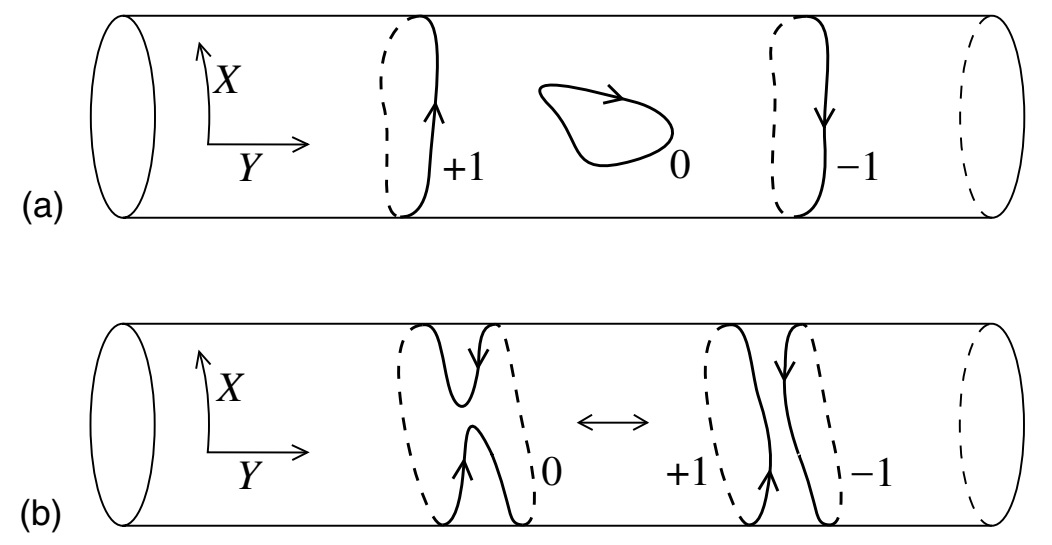
\includegraphics[width=0.8\textwidth]{figure/Fig8.1.jpg}
		\caption{(a) Oriented closed strings with winding numbers $w=+1,0,-1$.
			(b) Transition of a $w=0$ string into $w=+1$ and $w=-1$ strings.}\label{Fig8.1}
	\end{center}
\end{figure}

The second effect is unique to string theory. Closed strings can now wind around the compact dimension:
\begin{equation}
	X(\sigma+2 \pi)=X(\sigma)+2 \pi R w, \quad w \in \mathds{Z} \:. \label{8.2.3}
\end{equation}
The integer $w$ is the winding number.
States with winding numbers $+1, 0, -1$ are shown in Figure \ref{Fig8.1}(a).
From the viewpoint of worldsheet field theory, strings with non-zero winding number are topological solitons, i.e., states with topologically non-trivial field configurations. Consistent string theory must incorporate winding number states: through split-merge processes, 
$w=0$ strings can become $w=+1$ and $w=-1$ strings, as shown in Figure \ref{Fig8.1}(b). It is easy to see that winding number is always conserved in this example.
To determine the states of the closed string CFT, examine the Laurent expansion:
\begin{equation}
	\partial X(z)=-\mi\left(\frac{\alpha^{\prime}}{2}\right)^{1 / 2} \sum_{m=-\infty}^{\infty} \frac{\alpha_{m}}{z^{m+1}}\:, \qquad 
	\bar{\partial} X(\bar{z})=-\mi\left(\frac{\alpha^{\prime}}{2}\right)^{1 / 2} \sum_{m=-\infty}^{\infty} \frac{\tilde{\alpha}_{m}}{\bar{z}^{m+1}} \:. \label{8.2.4}
\end{equation}
After winding once, the change in $X$ is:
\begin{equation}
	2 \pi R w=\oint(\dif z\: \partial X + \dif \bar{z}\: \bar{\partial} X)= 2 \pi(\alpha^{\prime}/2)^{1/2}(\alpha_{0}-\tilde{\alpha}_{0}) \:. \label{8.2.5}
\end{equation}
The total Noether momentum is:
\begin{equation}
	p=\frac{1}{2 \pi \alpha^{\prime}} \oint(\dif z\: \partial X- \dif \bar{z}\: \bar{\partial} X)
	=(2 \alpha^{\prime})^{-1 / 2}(\alpha_{0}+\tilde{\alpha}_{0}) \:. \label{8.2.6}
\end{equation}
For non-compact dimensions, this gives $\alpha_{0}=\tilde{\alpha}_{0}=p(\alpha^{\prime} / 2)^{1 / 2}$ as usual, but for periodic dimensions we have:
\begin{subequations} \label{8.2.7}
	\begin{align}
		p_{L} \equiv\left(2 / \alpha^{\prime}\right)^{1 / 2} \alpha_{0}=\frac{n}{R}+\frac{w R}{\alpha^{\prime}} \:, \label{8.2.7a} \\
		p_{R} \equiv\left(2 / \alpha^{\prime}\right)^{1 / 2} \tilde{\alpha}_{0}=\frac{n}{R}-\frac{w R}{\alpha^{\prime}} \:. \label{8.2.7b}
	\end{align}		
\end{subequations}
The Virasoro generators are:
\begin{subequations} \label{8.2.8}
	\begin{align}
		L_{0}&=\frac{\alpha^{\prime} p_{L}^{2}}{4}+\sum_{n=1}^{\infty} \alpha_{-n} \alpha_{n} \:, \label{8.2.8a} \\
		\tilde{L}_{0}&=\frac{\alpha^{\prime} p_{R}^{2}}{4}+\sum_{n=1}^{\infty} \tilde{\alpha}_{-n} \tilde{\alpha}_{n} \:. \label{8.2.8b}
	\end{align}		 				
\end{subequations}

\subsection*{Partition Function}
The partition function for $X$ is:
\begin{align}
	&(q \bar{q})^{-1 / 24} \operatorname{Tr}\Bigl(q^{L_{0}} \bar{q}^{\tilde{L}_{0}}\Bigr) \nonumber \\
	&\quad =|\eta(\tau)|^{-2} \sum_{n, w=-\infty}^{\infty} q^{\alpha^{\prime} p_{L}^{2} / 4} \bar{q}^{\alpha^{\prime} p_{R}^{2} / 4} \nonumber \\
	&\quad =|\eta(\tau)|^{-2} \sum_{n, w=-\infty}^{\infty} \exp \left[-\pi \tau_{2}\left(\frac{\alpha^{\prime} n^{2}}{R^{2}}+\frac{w^{2} R^{2}}{\alpha^{\prime}}\right)+2 \pi \mi \tau_{1} n w\right] \:. \label{8.2.9}
\end{align}
The oscillators are the same as in the non-compact case, while the momentum integral is replaced by a sum over $n$ and $w$. Modular invariance is not obvious, but using the Poisson resummation formula:
\begin{equation}
	\sum_{n=-\infty}^{\infty} \exp (-\pi a n^{2}+2 \pi \mi b n)=a^{-1 / 2} 
	\sum_{m=-\infty}^{\infty} \exp \biggl[-\frac{\pi(m-b)^{2}}{a}\biggr] \:. \label{8.2.10}
\end{equation}
\begin{tcolorbox}[breakable]
	\begin{proof}
		Poisson resummation formula relates:
		\begin{align*}
			\sum_{n=-\infty}^{\infty} f(n) = \sum_{k=-\infty}^{\infty} \hat{f}(k) \tag{8.88}
		\end{align*}		
		where \(\hat{f}(k) = \int_{-\infty}^{\infty} dx \, e^{-2\pi i x k} f(x)\) is the Fourier transform of \(f(x)\). In our case we have
		\begin{align*}
			\hat{f}(k) &= \int_{-\infty}^{\infty} dx \, e^{-2\pi i x k} e^{-\pi a x^2 + 2\pi ibx} \\
			&= \int_{-\infty}^{\infty} dx \, e^{-\pi a x^2 + 2\pi i (b-k)x} \\
			&= \sqrt{\frac{\pi}{\pi a}} \, e^{\frac{-4\pi^2 (b-k)^2}{4\pi a}} \\
			&= a^{-1/2} e^{\frac{-\pi (b-k)^2}{a}} \tag{8.89}
		\end{align*}
		where we have used the Gaussian integral
		\begin{align*}
			\int_{-\infty}^{\infty} dx \, e^{-\alpha x^2 + \beta x} = \sqrt{\frac{\pi}{\alpha}} \, e^{\frac{\beta^2}{4\alpha}}
		\end{align*}
		Thus
		\begin{align*}
			\sum_{n=-\infty}^{\infty} \exp\left(-\pi a n^2 + 2\pi i b n\right) 
			= a^{-1/2} \sum_{m=-\infty}^{\infty} \exp\left[-\frac{\pi (m-b)^2}{a}\right]
		\end{align*}
	\end{proof}
\end{tcolorbox}
The partition function becomes:
\begin{equation}
	2 \pi R Z_{X}(\tau) \sum_{m, w=-\infty}^{\infty} \exp \biggl(-\frac{\pi R^{2}|m-w \tau|^{2}}{\alpha^{\prime} \tau_{2}}\biggr) \:. \label{8.2.11}
\end{equation}
$Z_{X}(\tau)$ is the modular invariant expression \eqref{7.2.9} for the non-compact theory; this sum is clearly invariant under $\tau \rightarrow \tau+1$. Under $\tau \rightarrow-1 / \tau$, it is invariant under $m\to-w$ and $w\to m$.

\begin{tcolorbox}[breakable]
	\begin{proof}
	The Poisson summation formula with \( a = \alpha' \tau_2 / R^2 \) and \( b = w \tau_1 \) on \eqref{8.2.9} becomes:
	\begin{align*}
		(q\bar{q})^{-1/24} \text{Tr } q^{L_0} \bar{q}^{\tilde{L}_0} 
		&= |\eta(\tau)|^{-2} \sum_{w=-\infty}^{\infty} \exp\left(-\frac{\pi \tau_2 R^2 w^2}{\alpha'} \right) \\
		&\quad \times \left( \frac{\alpha' \tau_2}{R^2} \right)^{-1/2} \sum_{m=-\infty}^{\infty} \exp\left[-\frac{\pi(m - w \tau_1)^2}{\alpha' \tau_2 / R^2}\right] \\
		&= |\eta(\tau)|^{-2} \frac{R}{(\alpha' \tau_2)^{1/2}} \sum_{m,w=-\infty}^{\infty} e^{-\frac{\pi R^2}{\alpha' \tau_2} \left[\tau_2^2 w^2 + (m-w \tau_1)^2\right]} \\
		&= |\eta(\tau)|^{-2} \frac{R}{(\alpha' \tau_2)^{1/2}} \sum_{m,w=-\infty}^{\infty} e^{-\frac{\pi R^2}{\alpha' \tau_2} \left[w^2 (\tau_1^2 + \tau_2^2) + m^2 - 2mw \tau_1\right]} 
	\end{align*}	
	Note now that
	\begin{align*}
		|m - w \tau|^2 &= (m - w \tau)(m - w \bar{\tau}) \\
		&= m^2 + w^2 |\tau|^2 - m w (\tau + \bar{\tau}) \\
		&= m^2 + w^2 (\tau_1^2 + \tau_2^2) - 2m w \tau_1 
	\end{align*}	
	and thus
	\begin{align*}
		(q\bar{q})^{-1/24} \text{Tr } q^{L_0} \bar{q}^{\tilde{L}_0} 
		= |\eta(\tau)|^{-2} \frac{R}{(\alpha' \tau_2)^{1/2}} \sum_{m,w=-\infty}^{\infty} e^{-\frac{\pi R^2 |m-w \tau|^2}{\alpha' \tau_2}} 
	\end{align*}
	We use \eqref{7.2.9}, i.e. \(|\eta(\tau)|^{-2} = (4\pi^2 \alpha' \tau_2)^{1/2} Z_X(\tau)\) to find
	\begin{align*}
		(q\bar{q})^{-1/24} \text{Tr } q^{L_0} \bar{q}^{\tilde{L}_0} 
		&= (4\pi^2 \alpha' \tau_2)^{1/2} Z_X(\tau) \frac{R}{(\alpha' \tau_2)^{1/2}} \sum_{m,w=-\infty}^{\infty} e^{-\frac{\pi R^2 |m-w \tau|^2}{\alpha' \tau_2}} \\
		&= 2\pi R Z_X(\tau) \sum_{m,w=-\infty}^{\infty} e^{-\frac{\pi R^2 |m-w \tau|^2}{\alpha' \tau_2}} 
	\end{align*}	
	Under \( \tau \to -1/\tau \) we have \( \tau_1 \to -\tau_1/|\tau|^2 \) and \( \tau_2 \to \tau_2/|\tau|^2 \). Thus
	\begin{align*}
		\sum_{m,w} \exp\left(-\frac{\pi R^2}{\alpha'} \frac{|m-w\tau|^2}{\tau_2}\right) 
		&\to \sum_{m,w} \exp\left(-\frac{\pi R^2}{\alpha'} \frac{|m+w/\tau|^2}{\tau_2/|\tau|^2}\right) \\
		&= \sum_{m,w} \exp\left(-\frac{\pi R^2}{\alpha'} \frac{|m\tau+w|^2}{\tau_2}\right) \\
		&= \sum_{w,m} \exp\left(-\frac{\pi R^2}{\alpha'} \frac{|-w\tau+m|^2}{\tau_2}\right)
	\end{align*}
	In the last line we have set \( w' = -m \) and \( m' = w \).
	\end{proof}
\end{tcolorbox}

\eqref{8.2.11} has a simple path integral interpretation.
Summing over all genus 1 worldsheets in periodic spacetime, each non-trivial closed curve on the worldsheet winds around the compact direction:
\begin{subequations} \label{8.2.12}
	\begin{align}
		X(\sigma^{1}+2 \pi, \sigma^{2}) &= X(\sigma^{1}, \sigma^{2})+2 \pi w R \:, \label{8.2.12a} \\
		X(\sigma^{1}+2 \pi \tau_{1}, \sigma^{2}+2 \pi \tau_{2}) &= X(\sigma^{1}, \sigma^{2})+2 \pi m R \:. \label{8.2.12b} 
	\end{align}
\end{subequations}
That is, the path integral splits into topologically inequivalent sectors labeled by $w$ and $m$. By writing $X$ as a classical solution satisfying periodicity:
\begin{equation}
	X_{\mathrm{cl}}=\sigma^{1} w R+\sigma^{2}(m-w \tau_{1}) R / \tau_{2} \:, \label{8.2.13}
\end{equation}
plus a quantum part satisfying periodic boundary conditions.
This Gaussian path integral can be integrated out. The path integral for the quantum part is the same as in the non-compact case, while the classical part appears as the exponential in \eqref{8.2.11}. The effect of modular transformations on periodicity is simplified to swapping the summation variables $m$ and $w$.

\subsection*{Vertex Operators}
To construct winding states with $\alpha_{0} \neq \tilde{\alpha}_{0}$, we need independent variables $x_{L}$ and $x_{R}$ satisfying:
\begin{equation}
	[x_{L}, p_{L}]=[x_{R}, p_{R}]=\mi \:. \label{8.2.14}
\end{equation}
The field $X$ splits into holomorphic and anti-holomorphic parts:
\begin{equation}
	X(z, \bar{z})=X_{L}(z)+X_{R}(\bar{z}) \:, \label{8.2.15}
\end{equation}
where:
\begin{subequations} \label{8.2.16}
	\begin{align}
		X_{L}(z) &= x_{L}- \mi \frac{\alpha^{\prime}}{2} p_{L} \ln z+\mi\left(\frac{\alpha^{\prime}}{2}\right)^{1 / 2} 
		\sum_{m=-\infty \atop m \neq 0}^{\infty} \frac{\alpha_{m}}{m z^{m}} \:, \label{8.2.16a} \\
		X_{R}(\bar{z})&= x_{R}-\mi \frac{\alpha^{\prime}}{2} p_{R} \ln \bar{z}+\mi\left(\frac{\alpha^{\prime}}{2}\right)^{1 / 2} 
		\sum_{m=-\infty \atop m \neq 0}^{\infty} \frac{\tilde{\alpha}_{m}}{m \bar{z}^{m}} \:. \label{8.2.16b}
	\end{align}
\end{subequations}
If we restrict to states with $k_{L}=k_{R}$ and only use operators constructed from $X_{L}(z)+X_{R}(\bar{z})$, this reduces to the CFT of non-compact dimensions. Note that $\ln|z|$ does not have any branch cut, however $\ln(z)$ does. As a result, $X^{\mu}$'s multivalued-ness is inherited by the mode decomposition.

We now discuss OPEs and vertex operators. The form of the vertex operator is easily guessed, since the usual $XX$ operator product $-(\alpha^{\prime} / 2) \ln (z_{12} \bar{z}_{12})$ can be split into holomorphic and anti-holomorphic functions, thus:
\begin{subequations} \label{8.2.17}
	\begin{align}
		X_{L}(z_{1}) X_{L}(z_{2}) &\sim-\frac{\alpha^{\prime}}{2} \ln z_{12}, \quad 
		X_{R}(\bar{z}_{1}) X_{R}(\bar{z}_{2}) \sim-\frac{\alpha^{\prime}}{2} \ln \bar{z}_{12}  \:,  \label{8.2.17a} \\
		X_{L}(z_{1}) X_{R}(\bar{z}_{2}) &\sim 0 \:. \label{8.2.17b}
	\end{align}		
\end{subequations}
The operator corresponding to the state $|0 ; k_{L}, k_{R}\rangle$ is:
\begin{equation}
	\mathscr{V}_{k_{L} k_{R}}(z, \bar{z}) = : \mathrel{e^{\mi k_{L} X_{L}(z)+ \mi k_{R} X_{R}(\bar{z})}}: \label{8.2.18}
\end{equation}
The OPE is:
\begin{equation}
	\mathscr{V}_{k_{L} k_{R}}(z_{1}, \bar{z}_{1}) \mathscr{V}_{k_{L}^{\prime} k_{R}^{\prime}}(z_{2}, \bar{z}_{2}) \sim 
	z_{12}^{\alpha^{\prime} k_{L} k_{L}^{\prime} / 2} \bar{z}_{12}^{\alpha^{\prime} k_{R} k_{R}^{\prime} / 2} 
	\mathscr{V}_{(k+k^{\prime})_{L}(k+k^{\prime})_{R}}(z_{2}, \bar{z}_{2}) \:. \label{8.2.19}
\end{equation}
We will encounter branch points and cuts in various expressions; this is not surprising, as the field \textbf{$X$ is no longer single-valued} as the boundary condition being imposed \eqref{8.2.3} has changed. However, it is important that the OPE of the entire vertex operator must be single-valued: when $z_{1}$ winds around $z_{2}$ once, the net phase is 1.
\begin{equation}
	\exp [\pi \mi \alpha^{\prime}(k_{L} k_{L}^{\prime}-k_{R} k_{R}^{\prime})]
	=\exp [2 \pi \mi(n w^{\prime}+w n^{\prime})]=1 \:. \label{8.2.20}
\end{equation}
This is exactly what is necessary for the string amplitude to be well-defined.

\subsection*{A Trick}

The previous discussion is clearly correct, but we have been too casual about the handling of branch points and cuts in the logarithms.
If we swap $z_{1}$ and $z_{2}$, and the momenta $k$ and $k^{\prime} $, a problem arises in OPE \eqref{8.2.19}. The left side is symmetric, but the right side will differ by $\exp[\pi \mi(n w^{\prime}+w n^{\prime})]$.
Therefore, if $n w^{\prime}+w n^{\prime}$ is odd, there will be a negative sign difference. We can also see this problem in the following way. From the mode expansion, we can derive the equal-time $(|z_{1}|=|z_{2}|)$ commutator:
\begin{equation}
	[X_{L}(z_{1}), X_{L}(z_{2})]=\frac{\pi \mi \alpha^{\prime}}{2} \operatorname{sign}(\sigma_{1}^{1}-\sigma_{2}^{1}) \:. \label{8.2.21}
\end{equation}
\begin{tcolorbox}[breakable]
	\begin{proof}
		We chose the worldsheet coordinate \( \sigma^1 \) to be in the range \([-\pi, \pi]\); it still has periodicity \( 2\pi \). Defining as usual \( z = e^{-iw} = e^{-i\sigma^1 + \sigma^2} \) we thus have \( \ln z = -i\sigma^1 + \sigma^2 \) and thus \( \sigma^1 = -\Im \ln z \). The logarithm has a branch cut that we put on the negative real axis. Working out \([X_L(z_1), X_L(z_2)]\), the only non-zero commutation relations we have are \([x_L, p_L] = i\) and \([\alpha_m, \alpha_n] = m\delta_{m+n}\). Thus
		
		\begin{align*}
			[X_L(z_1), X_L(z_2)] &= \left[ x_L - i \frac{\alpha'}{2} p_L \ln z_1 + i \sqrt{\frac{\alpha'}{2}} \sum_{m \neq 0} \frac{\alpha_m}{mz_1^m},\right. \\
			&\qquad \left. x_L - i \frac{\alpha'}{2} p_L \ln z_2 + i \sqrt{\frac{\alpha'}{2}} \sum_{n \neq 0} \frac{\alpha_n}{nz_2^n} \right] \\
			&= -i \frac{\alpha'}{2} \ln z_2 [x_L, p_L] - i \frac{\alpha'}{2} \ln z_1 [p_L, x_L] - \frac{\alpha'}{2} \sum_{m,n \neq 0} \frac{[\alpha_m, \alpha_n]}{mnz_1^m z_2^n} \\
			&= \frac{\alpha'}{2} \left( \ln z_2 - \ln z_1 - \sum_{m,n \neq 0} \frac{m\delta_{m+n}}{mnz_1^m z_2^n} \right) \\
			&= \frac{\alpha'}{2} \left( \ln z_2 - \ln z_1 - \sum_{n \neq 0} \frac{z_1^n}{nz_2^n} \right)
		\end{align*}
		
		Now from \(\ln(1-x) = -\sum_{n=1}^\infty x^n / n\) we have
		
		\begin{align*}
			\ln \left( 1 - \frac{z_1}{z_2} \right) - \ln \left( 1 - \frac{z_2}{z_1} \right) &= -\sum_{n=1}^\infty \frac{z_1^n}{nz_2^n} + \sum_{n=1}^\infty \frac{z_2^n}{nz_1^n} \\
			&= -\sum_{n=1}^\infty \frac{z_1^n}{nz_2^n} - \sum_{m=-\infty}^{-1} \frac{z_1^m}{mz_2^m} \\
			&= -\sum_{n \neq 0} \frac{z_1^n}{nz_2^n}
		\end{align*}
		
		and thus
		
		\begin{align*}
			[X_L(z_1), X_L(z_2)] &= \frac{\alpha'}{2} \left[ \ln z_2 - \ln z_1 + \ln \left( 1 - \frac{z_1}{z_2} \right) - \ln \left( 1 - \frac{z_2}{z_1} \right) \right] \\
			&= \frac{\alpha'}{2} \left[ \ln z_2 - \ln z_1 + \ln \frac{(z_2 - z_1)/z_2}{(z_1 - z_2)/z_1} \right] \\
			&= \frac{\alpha'}{2} \left[ \ln z_2 - \ln z_1 + \ln \left( -\frac{z_1}{z_2} \right) \right]
		\end{align*}
		Using \( z = e^{-i\sigma^1 + \sigma^2} \) and the fact that we have equal time commutators, i.e. that \( \sigma_1^2 = \sigma_2^2 \) we have
		
		\begin{align*}
			[X_L(z_1), X_L(z_2)] &= \frac{\alpha'}{2} \left[ -i\sigma_2^1 +\cancel{ \sigma_2^2} + i\sigma_1^1 -\cancel{ \sigma_1^2}+ \ln \left( e^{\pm i\pi} \frac{e^{-i\sigma_1^1 + \cancel{\sigma_1^2}}}{e^{-i\sigma_2^1 + \cancel{\sigma_2^2}}} \right) \right] \\
			&= \frac{\alpha'}{2} \left( -i\sigma_2^1 + i\sigma_1^1 + \ln e^{\pm i\pi - i\sigma_1^1 + i\sigma_2^1} \right) \\
			&= i\frac{\alpha'}{2} \left( -\sigma^1_2 + \sigma_1^1 \pm \pi - \sigma_1^1 + \sigma^1_2 \right) = \pm \frac{\pi i\alpha'}{2}
		\end{align*}
		Let us examine the logarithm in more detail: \(\ln e^{i(\pm\pi - \sigma_1^1 + \sigma_2^1)}\). If \(\sigma_1^1 > \sigma_2^1\), then \(-\sigma_1^1 + \sigma_2^1 < 0\). In this case we need to take the \(+\) sign. The most negative extreme occurs when \(\sigma_1^1 = +\pi\) and \(\sigma_2^1 = -\pi\), giving \(-\sigma_1^1 + \sigma_2^1 = -2\pi\). This value lies on the branch cut of logarithm; we can bring it back into the range \([-\pi, \pi]\) by adding \(+\pi\).
		
		Conversely, if \(\sigma_1^1 < \sigma_2^1\), then \(-\sigma_1^1 + \sigma_2^1 > 0\). Here we need to take the \(-\) sign. The most positive extreme occurs when \(\sigma_1^1 = -\pi\) and \(\sigma_2^1 = +\pi\), giving \(-\sigma_1^1 + \sigma_2^1 = 2\pi\). This also lies on the branch cut; we can bring it back into the range \([-\pi, \pi]\) by subtracting \(\pi\).
		
		We thus conclude that, indeed,
		\begin{align*}
			[X_L(z_1), X_L(z_2)] = \frac{\pi i\alpha'}{2} \operatorname{sign}(\sigma_1^1 - \sigma_2^1)
		\end{align*}
		We now use \(\bar{z} = e^{+i\sigma^1 + \sigma^2}\) and the fact that we have equal time commutators, to find
		
		\begin{align*}
			[X_R(z_1), X_R(z_2)] &= \frac{\alpha'}{2} \left[ i\sigma_2^1 + \sigma_2^2 - i\sigma_1^1 - \sigma_1^2 + \ln \left( e^{\pm i\pi} \frac{e^{+i\sigma_1^1 + \sigma_1^2}}{e^{+i\sigma_2^1 + \sigma_2^2}} \right) \right] \\
			&= \frac{\alpha'}{2} \left( +i\sigma_2^1 - i\sigma_1^1 + \ln e^{\pm i\pi + i\sigma_1^1 - i\sigma^1_2} \right) = \pm \frac{\pi i\alpha'}{2}
		\end{align*}
		
		We work out the sign in the same way as before, but now as the argument of the logarithm is \(\ln e^{i(\pm\pi + \sigma_1^1 - \sigma_2^1)}\) and not \(\ln e^{i(\pm\pi - \sigma_1^1 + \sigma_2^1)}\) we have the rôle of \(\sigma_1^1\) and \(\sigma_2^1\) interchanged. Therefore
		
		\begin{align*}
			[X_R(z_1), X_R(z_2)] = -\frac{\pi i\alpha'}{2} \operatorname{sign}(\sigma_1^1 - \sigma_2^1)
		\end{align*}
		QED.
	\end{proof}
\end{tcolorbox}
The CBH formula then tells us that if we define the operator through a creation-annihilation order, then when $n w^{\prime}+w n^{\prime}$ is odd, the operator $\mathscr{V}_{k_{L} k_{R}}$ anticommutes with $\mathscr{V}_{k_{k}^{\prime} k_{R}^{\prime}}$. The invisible branch point/cut \eqref{8.2.20} becomes two visible ones.
The correct oscillator expression for the vertex operator is (with some ambiguity in the phase):
\begin{equation}
	\mathscr{V}_{k_{L} k_{R}}(z, \bar{z})=\exp [\pi \mi(k_{L}-k_{R})(p_{L}+p_{R}) \alpha^{\prime} / 4] 
	\mathrel{\typecolon \me^{\mi k_{L} X_{L}(z)+\mi k_{R} X_{R}(\bar{z})} \typecolon} \:, \label{8.2.22}
\end{equation}
where $p_L, p_R$ are operators as usual, and $k$ is a number (the momentum carried by the given vertex operator).
When $\mathscr{V}_{k_{L} k_{R}}$ and $\mathscr{V}_{k_{L}^{\prime} k_{R}^{\prime}}$ commute with each other, the extra factor is called cocycles, which gives an extra phase:
\begin{align}
	\exp \Bigl\{\pi \mi\Bigl[(k_{L}-k_{R})(k_{L}^{\prime}+k_{R}^{\prime})-(k_{L}^{\prime}-k_{R}^{\prime})(k_{L}+k_{R})\Bigr] 
	\alpha^{\prime} / 4\Bigr\}\quad &  \nonumber \\
	=\exp [\pi \mi(n w^{\prime}-w n^{\prime})] &\:, \label{8.2.23}
\end{align}
which removes the branch points and cuts.
In most cases, this complexity can be ignored, and the simpler expression from the previous paragraph can be used; cocycles only affect the relative signs of specific amplitudes.
\begin{tcolorbox}[breakable]
	\begin{proof}
		\begin{align}
			\mathscr{V}_{k_{L_1}k_{R_1}}(z_1,\bar z_1)\mathscr{V}_{k_{L_2}k_{R_2}}(z_2,\bar z_2)
			&= e^{i\pi(k_{L_1}-k_{R_1})(p_L+p_R)\alpha'/4}e^{ik_{L_1}X_L(z_1)+ik_{R_1}X_R(\bar{z}_1)} \nonumber\\
			&\quad \times e^{i\pi(k_{L_2}-k_{R_2})(p_L+p_R)\alpha'/4}e^{ik_{L_2}X_L(z_2)+ik_{R_2}X_R(\bar{z}_2)}\label{8.117}
		\end{align}
		
		The \( p \) are momentum operators, so they pick up the momentum component of everything that is to their right. This thus becomes
		
		\begin{align}
			\mathscr{V}_{k_{L_1}k_{R_1}}(z_1,\bar z_1)\mathscr{V}_{k_{L_2}k_{R_2}}(z_2,\bar z_2)
			&= e^{i\pi(k_{L_1}-k_{R_1})(k_{L_1}+k_{L_2}+k_{R_1}+k_{R_2})\alpha'/4}e^{ik_{L_1}X_L(z_1)+ik_{R_1}X_R(\bar{z}_1)} \nonumber\\
			&\quad \times e^{i\pi(k_{L_2}-k_{R_2})(k_{L_2}+k_{R_2})\alpha'/4}e^{ik_{L_2}X_L(z_2)+ik_{R_2}X_R(\bar{z}_2)} \nonumber\\
			&= e^{i\pi\left[(k_{L_1}-k_{R_1})(k_{L_1}+k_{L_2}+k_{R_1}+k_{R_2})+(k_{L_2}-k_{R_2})(k_{L_2}+k_{R_2})\right]\alpha'/4} \nonumber\\
			&\quad \times e^{ik_{L_1}X_L(z_1)+ik_{R_1}X_R(\bar{z}_1)}e^{ik_{L_2}X_L(z_2)+ik_{R_2}X_R(\bar{z}_2)}
		\end{align}
		
		Using \eqref{8.117}
		
		\begin{align}
			\mathscr{V}_{k_{L_1}k_{R_1}}(z_1,\bar z_1)\mathscr{V}_{k_{L_2}k_{R_2}}(z_2,\bar z_2)
			&= e^{i\pi\left[(k_{L_1}-k_{R_1})(k_{L_1}+k_{L_2}+k_{R_1}+k_{R_2})+(k_{L_2}-k_{R_2})(k_{L_2}+k_{R_2})\right]\alpha'/4} \nonumber\\
			&\quad \times (-)^{n_1w_2+w_1n_2}e^{ik_{L_2}X_L(z_2)+ik_{R_2}X_R(\bar{z}_2)}e^{ik_{L_1}X_L(z_1)+ik_{R_1}X_R(\bar{z}_1)} 
		\end{align}
		
		and re-introduce the cocycles and their inverse. This gives
		
		\begin{align}
			\mathscr{V}_{k_{L_1}k_{R_1}}(z_1,\bar z_1)\mathscr{V}_{k_{L_2}k_{R_2}}(z_2,\bar z_2)
			&= e^{i\pi\left[(k_{L_1}-k_{R_1})(k_{L_1}+k_{L_2}+k_{R_1}+k_{R_2})+(k_{L_2}-k_{R_2})(k_{L_2}+k_{R_2})\right]\alpha'/4} \nonumber\\
			&\quad \times (-)^{n_1w_2+w_1n_2}e^{-i\pi(k_{L_2}-k_{R_2})(k_{L_1}+k_{L_2}+k_{R_1}+k_{R_2})} \nonumber\\
			&\quad \times e^{-i\pi(k_{L_1}-k_{R_1})(k_{L_1}+k_{R_1})\alpha'/4}\,
			\mathscr{V}_{k_{L_2}k_{R_2}}(z_2,\bar z_2)\mathscr{V}_{k_{L_1}k_{R_1}}(z_1,\bar z_1) 
		\end{align}
		
		It remains to work out the phase:
		
		\begin{align}
			\mathscr{V}_{k_{L_1}k_{R_1}}(z_1,\bar z_1)\mathscr{V}_{k_{L_2}k_{R_2}}(z_2,\bar z_2)
			&= (-)^{n_1w_2+w_1n_2}e^{i\pi\left[(k_{L_1}-k_{R_1})(k_{L_2}+k_{R_2})-(k_{L_2}-k_{R_2})(k_{L_1}+k_{R_1})\right]\alpha'/4} \nonumber\\
			&\quad \times \mathscr{V}_{k_{L_2}k_{R_2}}(z_2,\bar z_2)\mathscr{V}_{k_{L_1}k_{R_1}}(z_1,\bar z_1) \nonumber\\
			&= (-)^{n_1w_2+w_1n_2}e^{i\pi(2k_{L_1}k_{R_2}-2k_{R_1}k_{L_2})\alpha'/4}\notag\\
			&\qquad\times\mathscr{V}_{k_{L_2}k_{R_2}}(z_2,\bar z_2)\mathscr{V}_{k_{L_1}k_{R_1}}(z_1,\bar z_1) 
		\end{align}
		
		We find
		
		\begin{align}
			k_{L_1}k_{R_2} - k_{R_1}k_{L_2}
			&= \left( \frac{n_1}{R} + \frac{w_1R}{\alpha'} \right) \left( \frac{n_2}{R} - \frac{w_2R}{\alpha'} \right) - \left( \frac{n_1}{R} - \frac{w_1R}{\alpha'} \right) \left( \frac{n_2}{R} + \frac{w_2R}{\alpha'} \right) \nonumber\\
			&= -2 \frac{n_1w_2 - w_1n_2}{\alpha'}
		\end{align}
		
		and thus
		
		\begin{align}
			\mathscr{V}_{k_{L_1}k_{R_1}}(z_1,\bar z_1)\mathscr{V}_{k_{L_2}k_{R_2}}(z_2,\bar z_2)
			&= (-)^{n_1w_2 + w_1n_2}e^{-i\pi(n_1w_2 - w_1n_2)}\,
			\mathscr{V}_{k_{L_2}k_{R_2}}(z_2,\bar z_2)\mathscr{V}_{k_{L_1}k_{R_1}}(z_1,\bar z_1) \nonumber\\
			&= (-)^{n_1w_2 + w_1n_2}(-)^{n_1w_2 - w_1n_2}\,
			\mathscr{V}_{k_{L_2}k_{R_2}}(z_2,\bar z_2)\mathscr{V}_{k_{L_1}k_{R_1}}(z_1,\bar z_1) \nonumber\\
			&= (-)^{2n_1w_2}\,
			\mathscr{V}_{k_{L_2}k_{R_2}}(z_2,\bar z_2)\mathscr{V}_{k_{L_1}k_{R_1}}(z_1,\bar z_1) \nonumber\\
			&= \mathscr{V}_{k_{L_2}k_{R_2}}(z_2,\bar z_2)\mathscr{V}_{k_{L_1}k_{R_1}}(z_1,\bar z_1)
		\end{align}
		
		as \( 2n_1w_2 \) is always even. We thus see that adding the cocycle indeed ensures that the vertex operators commute.
	\end{proof}
\end{tcolorbox}
The general $X^{\mu}$ path integral \eqref{6.2.18} factors into holomorphic and anti-holomorphic parts in an obvious way, allowing for the substitution:
\begin{equation}
	\prod_{i<j}^{n}|z_{i j}|^{\alpha^{\prime} k_{i} k_{j}} \to \prod_{i<j}^{n} z_{i j}^{\alpha^{\prime} k_{L i} k_{L j} / 2} 
	\bar{z}_{i j}^{\alpha^{\prime} k_{R i} k_{R j} / 2} \:, \label{8.2.24}
\end{equation}
and we can also replace the $2 \pi \delta(\sum k)$ from the non-compact integral over $x_{0}$ with:
\begin{equation}
	2 \pi R \delta_{\Sigma_{i} n_{i}, 0} \delta_{\Sigma_{i} w_{i}, 0} \:. \label{8.2.25}
\end{equation}
The exact expression \eqref{8.2.22} will yield some additional signs.

\subsection*{DDF Operators}

We have seen that exponential operators can be split into holomorphic and anti-holomorphic parts, which has many applications. We now use this to discuss the DDF operators mentioned at the end of Chapter 4.

We will work with light-cone coordinates $X^{\pm}=2^{-1 / 2}(X^{0} \pm X^{1})$, whose holomorphic part has the OPE (dropping the $L$ subscript):
\begin{equation}
	X^{+}(z) X^{-}(0) \sim \frac{\alpha^{\prime}}{2} \ln z, \qquad X^{+}(z) X^{+}(0) \sim X^{-}(z) X^{-}(0) \sim 0 \:. \label{8.2.26}
\end{equation}
\begin{tcolorbox}
	\begin{remark}
		\begin{align}
			X^{+}(z) X^{-}(0) &= 2^{-1}\left(X^{0}(z)+X^{\prime}(z)\right)\left(X^{0}(0)-X^{\prime}(0)\right) 
			= 2^{-1}\left(\frac{\alpha^{\prime}}{2} \ln z_{12}+\frac{\alpha^{\prime}}{2}\ln z_{12}\right)\notag\\
			&=\frac{\alpha^{\prime}}{2} \ln z_{12} \:. \label{8.2.27}
		\end{align}
	\end{remark}
\end{tcolorbox}
\noindent From this, it follows that the operator:
\begin{equation}
	V^{i}(n k_{0}, z)=\partial X^{i}(z) \me^{\mi n k_{0} X^{+}(z)}(2 / \alpha^{\prime})^{1 / 2} \label{8.2.28}
\end{equation}
is a $(1,0)$ primary field, where $i$ is a transverse index.
The OPE is:
\begin{align}
	V^{i}(n k_{0}, z) V^{j}(m k_{0}, 0) &\sim-\frac{\delta^{i j}}{z^{2}} \me^{\mi(n+m) k_{0} X^{+}(0)}  \nonumber \\
	&\quad -\frac{\mi n k_{0} \delta^{i j}}{z} \partial X^{+}(0) \me^{\mi(n+m) k_{0} X^{+}(0)} \:. \label{8.2.29}
\end{align}
Define the DDF operator as:
\begin{equation}
	A_{n}^{i}=\oint \frac{\dif z}{2 \pi} \, V^{i}(n k_{0}, z) \:. \label{8.2.30}
\end{equation}
Unless $n+m=0$, the $z^{-1}$ term in OPE \eqref{8.2.28} is a total derivative, so the DDF operators satisfy the oscillator algebra:
\begin{equation}
	[A_{m}^{i}, A_{n}^{j}]=m \delta^{i j} \delta_{m,-n} \frac{\alpha^{\prime} k_{0} p^{+}}{2} \:. \label{8.2.31}
\end{equation}

Examine the action of this operator on a state with given momentum $q$. The vertex operator for $V^{i}(n k_{0}, z)$ and this state will contain $z^{-\alpha^{\prime} n k_{0} q^{-} / 2}$. 
Thus, if we fix $k_{0}=2 / \alpha^{\prime} q^{-}$, it will be single-valued. Then the contour integral \eqref{8.2.29} defines a reasonable operator in this sector.
The DDF operator is the integral of a $(1,0)$ tensor and thus commutes with the Virasoro generators, transforming physical states into physical states. From this, we can build physical states by acting on the oscillator ground state with DDF operators. 
The states obtained in this way correspond one-to-one with light-cone states. DDF operators do not contain $X^{-}$, so these states have no $\alpha_{-m}^{-}$ excitations. 
Thus, compared to the more general but less obvious construction in \eqref{4.4.19}, they actually yield the same states.

\section{\texorpdfstring{Closed Strings and $T$-duality}{8.3 Closed Strings and $T$-duality}} \label{sec:8.3}

Since we are studying string theory, we take $D=26$ and only assume $X^{25}$ is periodic.
The mass shell ($L_{0}$ and $\tilde{L}_{0}$) is:
\begin{align}
	m^{2}=-k^{\mu} k_{\mu} &= (k_{L}^{25})^{2}+\frac{4}{\alpha^{\prime}}(N-1) \nonumber \\
	&=(k_{R}^{25})^{2}+\frac{4}{\alpha^{\prime}}(\tilde{N}-1) \:, \label{8.3.1}
\end{align}
or:
\begin{subequations} \label{8.3.2}
	\begin{align}
		m^{2} &= \frac{n^{2}}{R^{2}}+\frac{w^{2} R^{2}}{\alpha^{\prime 2}}+\frac{2}{\alpha^{\prime}}(N+\tilde{N}-2) \:, \label{8.3.2a} \\
		0 &= n w+N-\tilde{N} \:. \label{8.3.2b} 
	\end{align}
\end{subequations}
There are four contributions to mass squared: compact momentum, winding string potential energy, oscillators, and zero-point energy. The discussion of the physical spectrum in Chapter 4 applies to any compactification, 
so we obtain the correct counting of states just by examining the transverse oscillators $M=2, \ldots, 25$.

First, we reproduce the field theory result for the massless spectrum. At a general value of $R$, states can only be massless when $n=w=0$ and $N=\tilde{N}=1$.
There are $24^{2}$ identical states, but it is useful to classify them based on whether the oscillators are in the spacetime direction $\mu$ or the internal direction 25:
\begin{align}
	&\alpha_{-1}^{\mu} \tilde{\alpha}_{-1}^{\nu}|0 ; k\rangle\:, \qquad 
	(\alpha_{-1}^{\mu} \tilde{\alpha}_{-1}^{25}+\alpha_{-1}^{25} \tilde{\alpha}_{-1}^{\mu})|0 ; k\rangle \:, \nonumber \\
	&(\alpha_{-1}^{\mu} \tilde{\alpha}_{-1}^{25}-\alpha_{-1}^{25} \tilde{\alpha}_{-1}^{\mu})|0 ; k\rangle\:, \qquad 
	\alpha_{-1}^{25} \tilde{\alpha}_{-1}^{25}|0 ; k\rangle \:. \label{8.3.3}
\end{align}
The first set further splits into the 25-dimensional graviton plus dilaton plus antisymmetric tensor. The second is the graviton on spacetime and internal indices, which is the Kaluza-Klein vector. The third is the vector from the antisymmetric tensor.
The last state is a scalar, which is the modulus of the radius in the compact direction; its vertex operator $:\mathrel{\partial X^{25} \bar{\partial} X^{25} \me^{\mi k \cdot X}}:$ is a perturbation of the metric $G_{25,25}$. This is the same spectrum found when examining low-energy field theory.

Examining the transformation of massive states under $U(1) \times U(1)$ symmetry is very beneficial.
Once again, Kaluza-Klein gauge symmetry comes from translations in the $X^{25}$ direction, 
so the corresponding charge is the compact momentum $p_{25} $. For antisymmetric tensor gauge symmetry, examine the zero-momentum vertex operator, which measures the transformation of any state coupled to it.
It is proportional to:
\begin{equation}
	\partial X^{\mu} \bar{\partial} X^{25}-\partial X^{25} \bar{\partial} X^{\mu}= 
	\bar{\partial}(X^{25} \partial X^{\mu})-\partial(X^{25} \bar{\partial} X^{\mu}) \:. \label{8.3.4}
\end{equation}
This is a total derivative, but on winding states, its integral is non-zero since $X^{25}$ is not single-valued. So the $B_{\mu, 25}$ charge is the winding number.
This is the first "stringy" physics we encounter in this compactification: no state carries this charge in field theory.

We verify the gauge coupling from the string three-point coupling. The gauge boson vertex operator is:
\begin{equation}
	\frac{2^{1 / 2} g_{\mathrm{c}, 25}}{\alpha^{\prime}}:\mathrel{(\partial X^{\mu} \bar{\partial} X^{25} \pm 
		\partial X^{25} \bar{\partial} X^{\mu}) \me^{\mi k \cdot X}}: \:. \label{8.3.5}
\end{equation}
We set the 25-dimensional string coupling $g_{\mathrm{c}, 25}=g_{\mathrm{c}}(2 \pi R)^{-1 / 2}$. The factor $(2 \pi R)^{-1 / 2}$ comes from the normalization of the zero-mode wave function. 
For general compact momentum and winding number, the tachyon vertex operator is:
\begin{equation}
	g_{\mathrm{c}, 25}:\mathrel{ \me^{\mi k_{L} \cdot X_{L}(z)+\mi k_{R} \cdot X_{R}(\bar{z})}}: \:. \label{8.3.6}
\end{equation}
The three-point amplitude for one gauge boson and two tachyons, if the compact momentum and winding number of the tachyons are non-zero, is similar to \eqref{6.6.14}:
\begin{align}
	& {-}2^{-1 / 2} \pi \mi g_{\mathrm{c}, 25}(2 \pi)^{25} \delta^{25}({\textstyle\sum_{i} k_{i}}) k_{23}^{\mu}
	(k_{L 23}^{25} \pm k_{R 23}^{25}) \nonumber \\
	\to & {-}2^{3 / 2} \pi \mi g_{\mathrm{c}, 25}(2 \pi)^{25} \delta^{25}({\textstyle \sum_{i} k_{i}}) k_{2}^{\mu}
	(k_{L 2}^{25} \pm k_{R 2}^{25}) \:. \label{8.3.7}
\end{align}
In the second line, we take the gauge boson momentum $k_{1} \rightarrow 0$, which defines the gauge coupling. Two gauge bosons couple to $k_{L 2}^{25} \pm k_{R 2}^{25}$ respectively, i.e., compact momentum and winding number. 
This is exactly what we expect. Replacing the gauge boson with a graviton and continuing to examine this amplitude, we reproduce the relationships between couplings in \eqref{8.1.11} and \eqref{8.1.12}, which are the same as those found in the effective action.

\subsection*{Enhanced Gauge Symmetry}

Thus far, everything is identical to field theory with one compact dimension. The 26-dimensional graviton yields the 25-dimensional graviton plus vector plus modulus. The only string effect is the winding state carrying the $B_{\mu, 25}$ charge.

Further and more magical effects come from special compact radii. We omitted the discussion of the massless spectrum previously; states are only massless at special values of the radius $R$.
The most enriched case is $R=\alpha^{1 / 2}$, 
so $k_{L, R}^{25}=(n \pm w) \alpha^{\prime-1 / 2}$, and the condition for massless states is:
\begin{equation}
	(n+w)^{2}+4 N=(n-w)^{2}+4 \tilde{N}=4 \:. \label{8.3.8}
\end{equation}
Besides the general solution $n=w=0, N=\tilde{N}=1$, we now have:
\begin{equation}
	n=w=\pm 1,\: N=0,\: \tilde{N}=1\:, \quad n=-w=\pm 1, \: N=1, \:\tilde{N}=0 \:, \label{8.3.9}
\end{equation}
as well as:
\begin{equation}
	n=\pm 2,\: w=N=\tilde{N}=0\:, \quad w=\pm 2, \: n=N=\tilde{N}=0 \:. \label{8.3.10}
\end{equation}

States in \eqref{8.3.9} introduce four gauge bosons, with vertex operators:
\begin{equation}
	: \mathrel{\bar{\partial} X^{\mu} \me^{\mi k \cdot X} \exp [\pm 2 \mi \alpha^{\prime-1 / 2} X_{L}^{25}]}: \:, \quad 
	: \mathrel{ \partial X^{\mu} \me^{\mi k \cdot X} \exp [\pm 2 \mi \alpha^{\prime-1 / 2} X_{R}^{25}]}: \:. \label{8.3.11}
\end{equation}
The exact definition of the exponential operator is the same as in the previous section. These states possess internal momentum and winding number, so they carry Kaluza-Klein charge and antisymmetric tensor gauge charge. The only consistent theory for charged massless vectors is a non-Abelian gauge theory, 
so the new gauge bosons must combine with the old gauge bosons to form a non-Abelian theory. It is now convenient to treat the previous vectors using $\partial X^{25} \bar{\partial} X^{\mu}$ and $\partial X^{\mu} \bar{\partial} X^{25}$. 
The first one couples to $k_{L}^{25}$; under this coupling, the first pair of states in \eqref{8.3.11} carries charge $\pm 1$, while the second pair is neutral. 
The second couples to $k_{R}^{25}$, and so on.
This indicates that the gauge group is $S U(2) \times S U(2)$; the three vectors containing $\bar{\partial} X^{\mu}$ constitute an $S U(2)$. 
The other three constitute another $S U(2)$.
To present this $S U(2) \times S U(2)$, define three $(1,0)$ currents:
\begin{subequations} \label{8.3.12}
	\begin{align}
		j^{1}(z)&=: \mathrel{\cos [2 \alpha^{-1 / 2} X_{L}^{25}(z)]}: \:, \label{8.3.12a}  \\
		j^{2}(z)&=:\mathrel{ \sin [2 \alpha^{\prime-1 / 2} X_{L}^{25}(z)]}: \:, \label{8.3.12b} \\
		j^{3}(z)&=\mi \partial X_{L}^{25}(z) / \alpha^{\prime 1 / 2} \:. \label{8.3.12c}
	\end{align}
\end{subequations}
They can be normalized such that the OPE is:
\begin{equation}
	j^{i}(z) j^{j}(0) \sim \frac{\delta^{i j}}{2 z^{2}}+ \mi \frac{\epsilon^{i j k}}{z} j^{k}(0) \:. \label{8.3.13}
\end{equation}
For $(0,1)$ currents $\tilde{\jmath}^{i} $, there are similar OPEs. 
The single-pole term implies the corresponding charges form an $SU(2)$ algebra. In fact, since these currents are holomorphic, there is an infinite-dimensional algebra formed by Laurent coefficients:
\begin{subequations} \label{8.3.14}
	\begin{align}
		j^{i}(z) &= \sum_{m=-\infty}^{\infty} \frac{j_{m}^{i}}{z^{m+1}}  \:, \label{8.3.14a} \\
		[j_{m}^{i}, j_{n}^{j}] &= \frac{m}{2} \delta_{m,-n} \delta^{i j}+ \mi \epsilon^{i j k} j_{m+n}^{k} \:, \label{8.3.14b} 
	\end{align}
\end{subequations}
which is called a current algebra, affine Lie algebra, or Kac-Moody algebra.
We will encounter such algebras frequently at the beginning of Chapter 11. It will be proven that the coefficient of $z^{-2}$ is quantized, 
and the value in \eqref{8.3.13} is the minimum. So this is called a level 1 $SU(2)$ current algebra.

This $S U(2) \times S U(2)$ symmetry shows for the first time that string theory perceives spacetime geometry in a way that is completely different from what we use in field theory, 
where only $U(1) \times U(1)$ symmetry is obvious at any radius. 
The origins of $j^{3}$ and $j^{1,2}$ are completely different—they are oscillator excitations and winding number-momentum excitations, respectively, 
and their representations in terms of $X^{25}$ are also completely different, but in their action on the string spectrum, they are related to each other by symmetry. Since the energy of internal momentum and winding number is cancelled by negative zero-point energy, the extra vectors are massless. 
This situation occurs not only in tachyon theory, but also in other cases in Volume II.

\subsection*{Scale and Coupling}

At the $S U(2) \times S U(2)$ radius, the relation \eqref{8.1.11} becomes:
\footnote{More accurately, this is a coupling for an $(n, w)=(1,0)$ state. Non-Abelian gauge bosons have $(|n|,|w|)=(1,1)$, 
	so their coupling is $g_{S U(2), 25}^{2}=4 \kappa_{25}^{2} / \alpha^{\prime}$, which is the traditional quantum physics definition of $SU(2)$ coupling. 
	We will see in Chapter 18 that this holds for all level 1 current algebras.}
\begin{equation}
	g_{25}^{2}=2 \kappa_{25}^{2} / \alpha^{\prime} \:. \label{8.3.15}
\end{equation}
If we compactify multiple dimensions, each dimension scales the same way. So, specifically, in 4 dimensions:
\begin{equation}
	g_{4}^{2}=2 \kappa_{4}^{2} / \alpha^{\prime} \:. \label{8.3.16}
\end{equation}
In nature, non-Abelian gauge couplings are of order 1, which implies that the string length $\alpha^{1 / 2}$ is not far from the gravitational length $\kappa_{4}$.

We can also think of this in the following way. The 4-dimensional gauge coupling is dimensionless, but the 4-dimensional gravitational coupling has dimensions. Define an effective dimensionless gravitational coupling, which depends on the energy scale $E$:
\begin{equation}
	g_{\mathrm{G}, 4}^{2}(E)=\kappa_{4}^{2} E^{2} \:, \label{8.3.17}
\end{equation}
which grows with the square of energy. Obviously, the dimensionless gauge coupling runs with energy, but this is slower than the dimensional scaling of gravitational coupling. 
Then by \eqref{8.3.16}, the string mass scale is where the gauge and gravitational couplings are roughly equal, 
$g_{\mathrm{G}, 4}^{2}(E) \approx g_{4}^{2}$.

It is also beneficial to examine the possibility of compactification to 4 dimensions, where some compactification dimensions might be much larger than others. This is best analyzed by starting from low energy and working up, where a dimensionless gauge coupling $g_{4}^{2}$ exists at low energy. 
At energy $\rho_{5}^{-1}$, one compact dimension becomes a visible dimension, and physics becomes 5-dimensional (for simplicity, we only examine this one dimension at this scale).
The effective 5-dimensional coupling is:
\begin{equation}
	g_{5}^{2}=2 \pi \rho_{5} g_{4}^{2} \:. \label{8.3.18}
\end{equation}
Similar to \eqref{8.1.12}, this originates from the effective action. The coupling $g_{5}^{2}$ has dimensions of length. That is, 5-dimensional Yang-Mills theory, like 4-dimensional gravity, is non-renormalizable. 
Correspondingly, the effective dimensionless coupling is:
\begin{equation}
	\hat{g}_{5}^{2}=g_{5}^{2} E=2 \pi \rho_{5} E g_{4}^{2} \:, \label{8.3.19}
\end{equation}
which grows linearly with energy. However, $g_{4}^{2}$ is not much less than 1 in nature, so the coupling becomes strong quickly at high energy; it is presumed that string theory is then required to make the short-distance behavior reasonable. 
So this compactification scale must be close to the gravitational scale. This analysis is modified in open string theory, where modern understandings of strong-coupling string theory are taken into account. 
There is a very low probability that string or Kaluza-Klein excitations are far below the Planck scale.

\subsection*{Higgs Mechanism}
Let $R$ move away from the $S U(2) \times S U(2)$ radius. It is most instructive to examine what happens. The extra gauge bosons now acquire mass:
\begin{equation}
	m=\sqrt{\frac{R^4+\alpha{'}\,^2-2R^2\alpha'}{R^2\alpha'^2}}=\frac{|R^{2}-\alpha^{\prime}|}{R \alpha^{\prime}} \approx \frac{2}{\alpha^{\prime}}\Bigl|R-\alpha^{\prime 1 / 2}\Bigr| \:, \label{8.3.20}
\end{equation}
where the approximation holds when the radius $R$ is very close to the $S U(2) \times S U(2)$ radius $\alpha^{\prime 1 / 2}$. Near this radius, the mass is much smaller than the string scale, and we should use low-energy field theory to understand the physics.

There is only one way to endow gauge bosons with such mass: spontaneous symmetry breaking, which is exactly what occurs. 
When $R=\alpha^{1 / 2}$, there are 10 massless scalars: the dilaton, the modulus $G_{25,25}$, the four states in \eqref{8.3.9}, and the four states in \eqref{8.3.10}, the latter nine generated by the vertex operators:
\begin{equation}
	: \mathrel{j^{i}(z) \tilde{\jmath}^{j}(\bar{z}) \me^{\mi k \cdot X(z, \bar{z})}}: \:. \label{8.3.21}
\end{equation}
Index $i$ is a vector under the left-moving $SU(2)$, and index $j$ is a vector under the right-moving $SU(2)$. That is, they transform according to the $(\bm{3},\bm{3})$ representation under $S U(2) \times S U(2) $. 
In particular, the modulus of the radius is $j^{3} \tilde{\jmath}^{3}$. 
Moving away from the $S U(2) \times S U(2)$ radius gives this field an expectation value, 
so the gauge symmetry is broken down to the $U(1) \times U(1)$ symmetry that preserves the $z$-axis. Indeed, this is exactly the gauge group at a general radius. 
Near the $SU(2)$ radius, 
the mass \eqref{8.3.20} is linear with respect to the modulus dimension $|R-\alpha^{\prime 1 / 2}|$, just like standard spontaneous breaking. 

We denote the spacetime fields corresponding to these nine scalar fields as $M_{i j} $. 
One variation in the modulus is $M_{33} \neq 0$, but near the $S U(2) \times S U(2)$ point, it is very instructive to investigate more general backgrounds. The interactions of these massless fields will be described by some spacetime action, and this action will contain a potential $U(M)$. 
These fields have no mass at the symmetry point, so there is no $M^{2}$ term in $U$, 
but there may be $(S U(2) \times S U(2))$-invariant cubic terms:
\begin{equation}
	U(M) \propto \epsilon^{i j k} \epsilon^{i^{\prime} j^{\prime} k^{\prime}} M_{i i^{\prime}} M_{j j^{\prime}} M_{k k^{\prime}}=\operatorname{det} M \:. \label{8.3.22}
\end{equation}
It is not difficult to prove from the three-point string amplitude that this term indeed exists. It is a cubic term for bosons and is unbounded from below, but like the tachyon, this is an artifact of bosonic string theory.

Ignoring the fact that this potential is unstable for small variations, it is meaningful to find its static classical solutions. To have a static background solution, the field equations for the graviton and dilaton require the potential to be zero, and the field equations for $M_{i j}$ require the potential to be stable:
\begin{equation}
	U(M)=\frac{\partial U(M)}{\partial M_{i j}}=0 \:. \label{8.3.23}
\end{equation}
Diagonalizing $M$ using $S U(2) \times S U(2)$ rotations, the condition \eqref{8.3.23} becomes:
\begin{equation}
	M_{11} M_{22} M_{33}=M_{11} M_{22}=M_{11} M_{33}=M_{22} M_{33}=0 \:. \label{8.3.24}
\end{equation}
Therefore, only one diagonal component can be non-zero. 
By $S U(2) \times S U(2)$ rotations, we can take this non-zero diagonal component to be $M_{33} $. So we have not constructed any physically new string background.

A continuous family of static background solutions is called a flat direction. There are nine massless scalars here, which can be reduced to three diagonal fields by $S U(2) \times S U(2)$ rotations, but there is only one flat direction (ignoring gauge equivalent directions). 
Of course, we only calculated the cubic terms in the fields, but in general, the cubic terms can be zero, while higher-order terms remain non-zero. To construct an exact flat direction, we need a more specialized discussion. 
That is, for any value of $R$, we can construct a free CFT. 
Note that if we consider $j^{1} \tilde{\jmath}^{1}$ or $j^{2} \tilde{\jmath}^{2}$ as moduli, since they are sines and cosines of $X^{25}$, the worldsheet action would look very complex, but since it is equivalent to the free theory obtained by varying $R$, the worldsheet theory is solvable.

\subsection*{$T$-duality}
From the mass formula:
\begin{equation}
	m^{2}=\frac{n^{2}}{R^{2}}+\frac{w^{2} R^{2}}{\alpha^{\prime 2}}+\frac{2}{\alpha^{\prime}}(N+\tilde{N}-2) \:, \label{8.3.25}
\end{equation}
we see that as $R \rightarrow \infty$, the mass of the winding states becomes infinite, while the compact momentum approaches a continuous spectrum, which is exactly what is expected for non-compact dimensions. Examine the opposite limit $R \rightarrow 0$. 
States with compact momentum acquire infinite mass, but the spectrum of winding states now approaches a continuum—winding strings around small circles does not cost too much energy. Thus, as the radius approaches zero, the spectrum approaches a continuum once again, just as in non-compact dimensions. 
This is completely different from field theory behavior, where there is only compact momentum $n$ and no winding number $w$, and at $R \rightarrow 0$, no state becomes light.

In fact, the limits $R \rightarrow 0$ and $R \rightarrow \infty$ are physically equivalent. 
The spectrum \eqref{8.3.25} is invariant under the following transformation:
\begin{equation}
	R \rightarrow R^{\prime}=\frac{\alpha^{\prime}}{R}, \quad n \leftrightarrow w \:. \label{8.3.26}
\end{equation}
This equivalence simultaneously extends to interactions. 
Note that swapping $n$ and $w$ is equivalent to:
\begin{equation}
	p_{L}^{25} \rightarrow p_{L}^{25}\:, \quad p_{R}^{25} \rightarrow-p_{R}^{25} \:. \label{8.3.27}
\end{equation}
Examine this theory at radius $R$. Recall the decomposition $X^{25}(z, \bar{z})=X_{L}^{25}(z)+X_{R}^{25}(\bar{z})$, and define:
\begin{equation}
	X^{\prime 25}(z, \bar{z})=X_{L}^{25}(z)-X_{R}^{25}(\bar{z}) \:. \label{8.3.28}
\end{equation}
The OPE and energy-momentum tensor of field $X^{\prime 25}$ are the same as those of $X^{25}$; negative signs will always appear in pairs. The only change to the CFT caused by replacing $X^{25}$ with $X^{\prime 25}$ is that it causes the sign change \eqref{8.3.27}, which will transform the spectrum of the theory at radius $R$ into the spectrum of the theory at radius $R^{\prime}$. That is, they are the same theory, just one written as $X^{25}$ and the other as $X^{\prime 25} $. 
This equivalence is called $T$-duality. That is, the $R \rightarrow 0$ limit and $R \rightarrow \infty$ are physically completely equivalent, which is completely different from the behavior of point particles, and this is another proof that the geometry of strings at short distances is completely different. The space of inequivalent theories is the ray $R \geq \alpha^{\prime 1 / 2} $. 
We could also take the range to be $0 \leq R \leq \alpha^{1 / 2}$, but taking the larger one is more natural: to us, the momentum continuum is more familiar than the winding continuum. 
And in the picture of larger $R$, the issue of locality will be clearer. Therefore, the smallest radius is the self-dual radius:
\begin{equation}
	R_{\text{self-dual}}=R_{SU(2) \times SU(2)}=\alpha^{\prime 1/2} \:. \label{8.3.29}
\end{equation}
The smallest distance scale is of the order of the string length.
This phenomenon will repeatedly appear in string perturbation theory, but non-perturbatively, we will see structures at even smaller scales. 

Many applications of $T$-duality are reflected in its non-trivial effect on the string dilaton $\Phi$. Examine the scattering amplitude of gravitons with neither winding nor compact momentum. These states are invariant under $T$-duality, so the amplitude must be as well. 
The latter can be read from the low-energy action \eqref{8.1.9}, so the 25-dimensional coupling $\kappa_{25}$ must be invariant under duality. 
And for the 26-dimensional coupling $\kappa=(2 \pi \rho)^{1 / 2} \kappa_{25}$, 
the effect of duality is:
\begin{equation}
	\rho^{\prime}=\frac{\alpha^{\prime}}{\rho}\:, \qquad \kappa^{\prime}=\frac{\alpha^{\prime 1 / 2}}{\rho} \kappa \:. \label{8.3.30}
\end{equation}
Since $\kappa \propto \me^{\Phi}$, this implies:
\begin{equation}
	\me^{\Phi^{\prime}}=\frac{\alpha^{1 / 2}}{\rho} \me^{\Phi} \:. \label{8.3.31}
\end{equation}

$T$-duality is a symmetry that relates different states (backgrounds) in a single theory; in fact, it is a gauge symmetry. We saw that the modulus $\delta R$ is the 33-component of the $(\bm{3},\bm{3})$ field. 
Rotating around the 1-axis of one of the $S U(2)$s by an angle $\pi$ reflects the sign of the modulus, so decreasing $R$ from the $S U(2) \times S U(2)$ radius is gauge equivalent to increasing $R$. 
Therefore, the $\mathds{Z}_{2}$ symmetry of duality is a small part of the $S U(2) \times S U(2)$ gauge symmetry. This further implies that duality is not only a symmetry of string perturbation theory, but also a symmetry of the exact theory. 
If we have massless gauge bosons in the leading approximation, even a small explicit breaking of symmetry would lead to inconsistency (spontaneous symmetry breaking is not a problem; at this point $T$-duality is already spontaneously broken, moving away from the self-dual radius).

The final discussion exemplifies an important idea: the mutual mapping of discussions on strings and spacetime. 
The appearance of enhanced symmetry is a pure string theory phenomenon. We do not have a non-perturbative understanding of string theory. 
But we know a lot about low-energy field theory, even non-perturbatively, and we can utilize this.

\section{\texorpdfstring{Compactification of Several Dimensions}{8.4 Compactification of Several Dimensions}} \label{sec:8.4}
Now extend the analysis to $k$ periodic dimensions:
\begin{equation}
	X^{m} \cong X^{m}+2 \pi R \:, \quad 26-k \leq m \leq  25 \:. \label{8.4.1}
\end{equation}
Let $d=26-k$ be the number of non-compact dimensions. Now spacetime is $M^{d} \times T^{k}$. Assume for now that the coordinate periodicity \eqref{8.4.1} remains unchanged, but the actual geometry of the $k$-torus actually depends on the internal metric $G_{m n}$. When the compact dimension is greater than 1, the antisymmetric tensor also has scalar components $B_{m n}$. This altogether gives $k^{2}$ scalars. 
There are also Kaluza-Klein gauge bosons $A_{\mu}^{m}$ and antisymmetric tensor gauge bosons $B_{m \mu}$. The low-energy effective action is:
\begin{align}
	\bm{S} &= \frac{(2 \pi R)^{k}}{2 \kappa_{0}^{2}} \int \dif^{d} x \: (-G_{d})^{1/2} \me^{-2 \Phi_{d}}
	\biggl[\bm{R}_{d}+4 \partial_{\mu} \Phi_{d} \partial^{\mu} \Phi_{d} \nonumber \\
	&\qquad -\frac{1}{4} G^{m n} G^{p q} (\partial_{\mu} G_{m p} \partial^{\mu} G_{n q}+\partial_{\mu} B_{m p} \partial^{\mu} B_{n q})  \nonumber \\
	&\qquad -\frac{1}{4} G_{m n} F_{\mu \nu}^{m} F^{n \mu \nu}-\frac{1}{4} G^{m n} H_{m \mu \nu} H_{n}^{\mu \nu}
	-\frac{1}{12} H_{\mu \nu \lambda} H^{\mu \nu \lambda}\biggr] \:, \label{8.4.2}
\end{align}
where $\Phi_{d}=\Phi-\frac{1}{4} \ln \operatorname{det} G_{m n}$.

\subsection*{String Spectrum}
The main new issue is the antisymmetric tensor background $B_{mn}$. The contribution of this term to the worldsheet Lagrangian density is proportional to:
\begin{equation}
	B_{m n} \partial_{a}(g^{1 / 2} \epsilon^{a b} X^{m} \partial_{b} X^{n}) \:, \label{8.4.3}
\end{equation}
which is a total derivative if $B_{m n}$ is constant. It has no local effect, and the worldsheet theory remains a CFT. 
But it changes the string spectrum. We will examine this using canonical methods and path integrals.

In canonical methods, focus on the contribution of zero modes to the worldsheet action:
\begin{equation}
	X^{m}(\sigma^{1}, \sigma^{2})=x^{m}(\sigma^{2})+w^{m} R \sigma^{1} \:, \label{8.4.4}
\end{equation}
substituting it into the worldsheet action:
\begin{equation}
	L=\frac{1}{2 \alpha^{\prime}} G_{m n}(\dot{x}^{m} \dot{x}^{n}+w^{m} w^{n} R^{2})
	-\frac{\mi}{\alpha^{\prime}} B_{m n} \dot{x}^{m} w^{n} R \:. \label{8.4.5}
\end{equation}
The dot represents differentiation with respect to worldsheet time $\sigma^{2}$. The canonical momentum is:
\begin{equation}
	p_{m}=-\frac{\partial L}{\partial v^{m}}=\frac{1}{\alpha^{\prime}}(G_{m n} v^{n}+B_{m n} w^{n} R) \:. \label{8.4.6}
\end{equation}
where $v^{m}=\mi \dot{x}^{m} $. Some less familiar notation appears because we used Euclidean time. 
Extended to Minkowski time, $v^{m}$ becomes the velocity $\partial_{0} x^{m} $. 
The periodicity of the wave function implies the quantization of canonical momentum, $p_{m}=n_{m} / R$, thus:
\begin{equation}
	v_{m}=\alpha^{\prime} \frac{n_{m}}{R}-B_{m n} w^{n} R \:. \label{8.4.7}
\end{equation}
The zero-mode contribution to the worldsheet Hamiltonian is:
\begin{equation}
	\frac{1}{2 \alpha^{\prime}} G_{m n}(v^{m} v^{n}+w^{m} w^{n} R^{2}) \:, \label{8.4.8}
\end{equation}
and the mass of the closed string is:
\begin{subequations} \label{8.4.9}
	\begin{align}
		m^{2} &= \frac{1}{2 \alpha^{\prime 2}} G_{m n}(v_{L}^{m} v_{L}^{n}+v_{R}^{m} v_{R}^{n})
		+\frac{2}{\alpha^{\prime}}(N+\tilde{N}-2)  \:, \label{8.4.9a} \\
		v_{L, R}^{m} &= v^{m} \pm w^{m} R \:. \label{8.4.9b}
	\end{align}
\end{subequations}
Therefore, since $v^{m}$ depends on $B_{m n}$, the $B_{m n}$ background shifts the mass of winding states. The $L_{0}-\tilde{L}_{0}$ constraint is:
\begin{align}
	0 &=G_{m n}(v_{L}^{m} v_{L}^{n}-v_{R}^{m} v_{R}^{n})+4 \alpha^{\prime}(N-\tilde{N}) \nonumber \\
	&=4 \alpha^{\prime}(n_{m} w^{m}+N-\tilde{N}) \:. \label{8.4.10}
\end{align}

On the other hand, consider the torus path integral for the partition function. The antisymmetric tensor term is locally a total derivative, so it only depends on the topology of the configuration. Consider the configuration:
\begin{equation}
	X^{m}=(w_{1}^{m} \sigma^{1}+w_{2}^{m} \sigma^{2}) R \:. \label{8.4.11}
\end{equation}
The spatial direction on the torus winds $w_{1}^{m}$ times around each periodic spacetime dimension, while the temporal direction winds $w_{2}^{m}$ times. 
The $B_{m n}$ worldsheet action is:
\begin{equation}
	2 \pi \mi b_{m n} w_{1}^{m} w_{2}^{n} \:, \label{8.4.12}
\end{equation}
where $b_{m n}=B_{m n} R^{2} / \alpha^{\prime}$. It can be proven through the Poisson resummation formula that summing over path integral sectors with phase \eqref{8.4.12} is related to the partition function with the shifted spectrum \eqref{8.4.9}. 
In the previous description, the metric $G_{m n}$ appears in the worldsheet field action. For vertex operator calculations, it is more convenient to retain the usual action. Write the metric in terms of the frame $e_{m}{}^{r}$:
\begin{equation}
	G_{m n}=e_{m}{}^{r} e_{n}{}^{r} \:, \label{8.4.13}
\end{equation}
where $r, s, \ldots$ are tangent space coordinates. The OPE of the coordinates $X^{r}=e_{m}{}^{r} X^{m}$ is standard. 
The vertex operator momentum is:
\begin{equation}
	k_{r L}=e_{r}{}^{m} \frac{v_{m L}}{\alpha^{\prime}}, \qquad k_{r R}=e_{r}{}^{m} \frac{v_{m R}}{\alpha^{\prime}} \:, \label{8.4.14}
\end{equation}
where $e_{r}{}^{m} $ is the inverse frame.
The mass-shell conditions become:
\begin{subequations} \label{8.4.15}
	\begin{align}
		m^{2} &=\frac{1}{2}(k_{r L} k_{r L}+k_{r R} k_{r R})+\frac{2}{\alpha^{\prime}}(N+\tilde{N}-2) \:, \label{8.4.15a} \\	
		0 &= \alpha^{\prime}(k_{r L} k_{r L}-k_{r R} k_{r R})+4(N-\tilde{N}) \:. \label{8.4.15b}
	\end{align}
\end{subequations}
In the following, we will use coordinates $X^{r}$ in any discussion of vertex operators.

\subsection*{Narain Compactification}
There is a very elegant description for general toroidal compactifications. Consider the winding state vertex operator $\me^{\mi k_{L} \cdot X_{L}+\mi k_{R} \cdot X_{R}}$. 
For any given compactification, the momentum spectrum $(k_{r L}, k_{r R})$ forms a lattice in the $2 k$-dimensional momentum space $\mathds{R}^{2 k}$. 
That is, the momentum spectrum consists of all linear combinations of $2 k$ mutually independent basis vectors with integer coefficients. 
We now work with dimensionless momentum $l_{L, R}=k_{L, R}(\alpha^{\prime}/2)^{1 / 2}$, 
and we denote the corresponding lattice as $\Gamma $. The OPE of two vertex operators is:
\begin{align}
	&:\mathrel{\me^{\mi k_{L} \cdot X_{L}(z)+\mi k_{R} \cdot X_{R}(\bar{z})} }: 
	:\mathrel{\me^{\mi k_{L}^{\prime} \cdot X_{L}(0)+i k_{R}^{\prime} \cdot X_{R}(0)}}: \nonumber \\
	&\qquad \qquad \sim z^{l_{L} \cdot l_{L}^{\prime}} \bar{z}^{l_{R} \cdot l_{R}^{\prime}}
	:\mathrel{ \me^{\mi(k_{L}+k_{L}^{\prime}) \cdot X_{L}(0)+\mi(k_{R}+k_{R}^{\prime}) \cdot X_{R}(0)} }: \:. \label{8.4.16}
\end{align}
When one vertex operator winds around another vertex operator once, this product yields the phase $\exp[2 \pi \mi(l_{L} \cdot l_{L}^{\prime}-l_{R} \cdot l_{R}^{\prime})]$. 
The single-valuedness of the operator product requires:
\begin{equation}
	l_{L} \cdot l_{L}^{\prime}-l_{R} \cdot l_{R}^{\prime} \equiv l \vysmwhtcircle l^{\prime} \in \mathds{Z} \:, \label{8.4.17}
\end{equation}
where $l$ and $l^{\prime}$ belong to $\Gamma$. 
We defined the inner product $\vysmwhtcircle$, which has signature $(k, k)$ in $\mathds{R}^{2 k} $. 
The dual lattice $\Gamma^{*}$ is defined as the set of points in $\mathds{R}^{2 k}$ with integer-valued $\vysmwhtcircle$ inner products with points in $\Gamma$. Then the single-valuedness condition is equivalent to:
\begin{equation}
	\Gamma \subset \Gamma^{*} \:. \label{8.4.18}
\end{equation}

Modular invariance also constrains $\Gamma $. 
It was proven in section 7.2 that invariance under $\tau \rightarrow \tau+1$ requires $L_{0}-\tilde{L}_{0}$ to be an integer. Then:
\begin{equation}
	l \vysmwhtcircle l \in 2 \mathds{Z} \quad \forall l \in \Gamma \:. \label{8.4.19}
\end{equation}
\begin{tcolorbox}
	\begin{remark}
		$L_0-\tilde{L}_0=\frac{\alpha^{\prime}}{4}(k_{r L} k_{r L}-k_{r R} k_{r_{R}})
		=\frac{1}{2}(l_{rL}l_{r R}-l_{r R} l_{rR})=\frac{1}{2} l \vysmwhtcircle l \:. \label{8.4.20}$ 
	\end{remark}
\end{tcolorbox}
\noindent \eqref{8.4.19} actually implies \eqref{8.4.17}, which is given by the closure of the OPE:
\begin{equation}
	2 l \vysmwhtcircle l^{\prime}=(l+l^{\prime}) \vysmwhtcircle (l+l^{\prime})-l \vysmwhtcircle l-l^{\prime} \vysmwhtcircle l^{\prime} \in 2 \mathds{Z} \:. \label{8.4.21}
\end{equation}
Modular invariance under $\tau \rightarrow-1 / \tau$ requires more careful calculation. The partition function of the compact dimension is:
\begin{equation}
	Z_{\Gamma}(\tau)=|\eta(\tau)|^{-2 k} \sum_{l \in \Gamma} \exp (\pi \mi \tau l_{L}^{2}-\pi \mi \tau l_{R}^{2}) \:. \label{8.4.22}
\end{equation}
To determine the transformation properties of $Z_{\Gamma}$, use Poisson resummation. Use:
\begin{equation}
	\sum_{l^{\prime} \in \Gamma} \delta(l-l^{\prime})=V_{\Gamma}^{-1} \sum_{l^{\prime \prime} \in \Gamma^{*}} 
	\exp (2 \pi \mi l^{\prime \prime}  \vysmwhtcircle l) \:. \label{8.4.23}
\end{equation}
Here, $V_{\Gamma}$ is the volume of the unit cell of lattice $\Gamma$. \eqref{8.4.23} is similar to a Fourier series: only when $l \in \Gamma$ does the phase average not vanish, and normalization is given by integration over the unit cell. 
Using \eqref{8.4.23}, the sum \eqref{8.4.22} can be written as:
\begin{align}
	Z_{\Gamma}(\tau) &=V_{\Gamma}^{-1}|\eta(\tau)|^{-2 k} \sum_{l^{\prime \prime} \in \Gamma^{*}} 
	\int \dif^{2 k} l \: \exp (2 \pi \mi l^{\prime \prime} \vysmwhtcircle l+ \pi \mi \tau l_{L}^{2} 
	-\pi \mi \bar{\tau} l_{R}^{2}) \nonumber \\
	&=V_{\Gamma}^{-1}(\tau \bar{\tau})^{-k / 2}|\eta(\tau)|^{-2 k} \sum_{l^{\prime \prime} \in \Gamma^{*}} 
	\exp (-\pi \mi l_{L}^{\prime \prime 2} / \tau+\pi \mi l_{R}^{\prime \prime 2} / \bar{\tau}) \nonumber \\
	&=V_{\Gamma}^{-1} Z_{\Gamma^{*}}(-1 / \tau) \:, \label{8.4.24}
\end{align}
where we used modular transformation \eqref{7.2.44} in the last line. 
Then the sufficient condition for modular invariance is:
\begin{equation}
	\Gamma=\Gamma^{*} \:, \label{8.4.25}
\end{equation}
Since $V_{\Gamma}=V_{\Gamma^{*}}^{-1}$, if \eqref{8.4.25} holds, it equals 1. If modular invariance holds for all $\tau$, it can further be proven that this is a sufficient condition.

Consistency conditions can be summarized in two requirements: $\Gamma$ is an even self-dual lattice with signature $(k, k)$; even refers to property \eqref{8.4.19}, and self-dual refers to \eqref{8.4.25}.

All such lattices have been classified. 
Note that consistency conditions \eqref{8.4.19} and \eqref{8.4.25} depend on momentum $l$ through the $\vysmwhtcircle$ product, 
which is invariant under Lorentz boosts in $2 k$-dimensional space, $O(k, k, \mathds{R})$ transformations. If $\Gamma$ is an even self-dual lattice, then:
\begin{equation}
	\Gamma^{\prime}=\Lambda \label{8.4.26}
\end{equation}
is also an even self-dual lattice, where $\Lambda $ is an $O(k, k, \mathds{R})$ transformation. Note that $O(k, k, \mathds{R})$ is not a symmetry of the theory. 
The mass-shell condition and operator product also contain individual dot products $l_{L} \cdot l_{L}^{\prime}$ and $l_{R} \cdot l_{R}^{\prime}$, thus they are only invariant under $O(k, \mathds{R}) \times O(k, \mathds{R})$. So, 
most $O(k, k, \mathds{R})$ transformations yield inequivalent theories. 
Examine the $k=1$ case, where:
\begin{equation}
	l_{L, R}=\frac{n}{r} \pm \frac{m r}{2} \:, \label{8.4.27}
\end{equation}
$r=R(2 / \alpha^{\prime})^{1 / 2}$ is the dimensionless radius. This is indeed an even self-dual lattice. 
The transformation:
\begin{equation}
	l_{L}^{\prime}=l_{L} \cosh \lambda+l_{R} \sinh \lambda\:, \quad l_{R}^{\prime}=l_{L} \sinh \lambda+l_{R} \cosh \lambda \label{8.4.28}
\end{equation}
transforms the lattice into one with $r^{\prime}=r \me^{-\lambda}$.

Given the Lorentz signature, all even self-dual lattices can be obtained from one lattice through $O(k, k, \mathds{R})$ transformations. 
Starting from a given solution, such as all compact dimensions being mutually orthogonal and at the $S U(2)$ radius with $B_{m n}=0 $. The corresponding momentum lattice $\Gamma_{0}$ is called $k P_{2}$ and yields the gauge group $S U(2)^{2 k}$. 
As discussed earlier, if $\Lambda^{\prime} \in O(k, \mathds{R}) \times O(k, \mathds{R})$, 
then two $O(k, k, \mathds{R})$ transformations $\Lambda$ and $\Lambda^{\prime} \Lambda$ yield equivalent string theories; so, 
the space of inequivalent theories obtained in this way is:
\begin{equation}
	\frac{O(k, k, \mathds{R})}{O(k, \mathds{R}) \times O(k, \mathds{R})} \:. \label{8.4.29}
\end{equation}
There are also some discrete equivalence relations, which we will discuss briefly later. 
This is equivalent to the description using $G_{m n}$ and $B_{m n} $ made earlier. In particular, the number of parameters in the coset \eqref{8.4.29} is:
\begin{equation}
	\frac{2 k(2 k-1)}{2}-k(k-1)=k^{2} \:, \label{8.4.30}
\end{equation}
which is the same as the number of components in $G_{m n}$ and $B_{m n}$. 
Compared with one-dimensional compactification, $T$-duality symmetry is greatly expanded. In this abstract description, $O(k, k, \mathds{R})$ has some discrete subgroups that transform the lattice $\Gamma_{0}$ into itself. 
These subgroups are customarily denoted as $O(k, k, \mathds{Z})$. 
If $\Lambda^{\prime \prime}$ belongs to this subgroup, then obviously $\Lambda \Gamma_{0}$ and $\Lambda \Lambda^{\prime \prime} \Gamma_{0}$ are the same lattice. 
In summary, we have the following equivalence relations:
\begin{subequations} \label{8.4.31}
	\begin{align}
		\Lambda \Gamma_{0} &\cong \Lambda^{\prime} \Lambda \Lambda^{\prime \prime} \Gamma_{0} \:, \label{8.4.31a} \\
		\Lambda^{\prime} &\in O(k, \mathds{R}) \times O(k, \mathds{R}), \quad \Lambda^{\prime \prime} \in O(k, k, \mathds{Z} ) \:. \label{8.4.31b}
	\end{align}
\end{subequations}
Then the space of inequivalent lattices and inequivalent backgrounds is:
\begin{equation}
	\frac{O(k, k, \mathds{R})}{O(k, \mathds{R}) \times O(k, \mathds{R}) \times O(k, k, \mathds{Z})} \:. \label{8.4.32}
\end{equation}
Note that the continuous group in the denominator is a left action, while the discrete group is a right action. 

From the form of the background, the $T$-duality group $O(k, k, \mathds{Z})$ contains several transformations. 
One is the $R \rightarrow \alpha^{\prime} / R$ duality on a single axis. 
Another is the large coordinate transformation reflecting periodicity:
\begin{equation}
	x^{\prime \prime m}=L^{m}{}_{n} x^{n} \:, \label{8.4.33}
\end{equation}
where $L^{m}{}_{n}$ are integers and $\operatorname{det}L=1$. This is the group $SL(k, \mathds{Z})$. 
The last is the shift in the antisymmetric tensor background:
\begin{equation}
	b_{m n} \rightarrow b_{m n}+N_{m n} \label{8.4.34}
\end{equation}
where $N_{m n}$ are integers. From canonical results \eqref{8.4.7} or path integral phases \eqref{8.4.12}, it can be seen that these leave the spectrum invariant. These together generate the entire $T$-duality group. 
For a general $\Lambda$, there are no $\Lambda_{1,2}$ in the denominator group such that $\Lambda_{1} \Lambda \Lambda_{2}=\Lambda$, so there is no $T$-duality that leaves points in the covering space fixed. 
At some special $\Lambda$, solutions to $\Lambda_{1} \Lambda \Lambda_{2}=\Lambda$ exist, and they are different points of the $T$-duality element $\Lambda_{2}$. 
In the one-dimensional case, we can find such points, which are also the points of enhanced gauge symmetry. In higher-dimensional cases, besides $SU(2)$, larger gauge groups appear at different points, which we will discuss further in Chapter 11.

When there is a moduli space parameterized by scalar fields $\phi^{i}$, the kinetic term:
\begin{equation}
	-\frac{1}{2} g_{i j}(\phi) \partial_{\mu} \phi^{i} \partial^{\mu} \phi^{j} \label{8.4.35}
\end{equation}
defines a natural metric on the moduli space. 
More precisely, a definite definition requires performing a Weyl transformation first, as in \eqref{3.7.25}, to make the coefficient of the gravitational action modulus-independent and eliminate the mixing between the modulus and the spacetime metric. 
In low-energy action \eqref{8.4.2}, the corresponding scalar kinetic term is proportional to:
\begin{equation}
	\frac{16}{d-2} \partial_{\mu} \Phi \partial^{\mu} \Phi+G^{m n} G^{p q}
	(\partial_{\mu} G_{m p} \partial^{\mu} G_{n q}+\partial_{\mu} B_{m p} \partial^{\mu} B_{n q}) \:. \label{8.4.36}
\end{equation}
The coset space \eqref{8.4.32} has a unique $O(k, k, \mathds{R})$-invariant metric, which is exactly the second term in \eqref{8.4.36}. 
This $O(k, k, \mathds{R})$ is not a symmetry of the entire theory; only its discrete $T$-duality subgroup $O(k, k, \mathds{Z})$ is. 
The difference between the two is invisible at low energy—it comes from the quantization of string zero modes, thus only affecting the massive spectrum. Therefore, $O(k, k, \mathds{R})$ is only an accidental symmetry of the low-energy theory. 
In this example, the moduli space is the product of the dilaton moduli space and the compactification moduli space.

\subsection*{Example}
Two compactification dimensions are a good example. The four moduli $G_{24,24}$, $G_{24,25}$, $G_{25,25}$, and $B_{24,25}$ are usually combined into two complex fields $\tau=\tau_{1}+\mi \tau_{2}$ and $\rho=\rho_{1}+\mi \rho_{2}$. 
Define:
\begin{align}
	\rho &= \frac{R^{2}}{\alpha^{\prime}}\Bigl(B_{24,25} + \mi \operatorname{det}^{1 / 2} G_{m n}\Bigr) \nonumber \\
	&= b_{24,25}+\mi \frac{V}{4 \pi^{2} \alpha^{\prime}} \:, \label{8.4.37}
\end{align}
where $V$ is the volume of the compact 2-torus. 
Parameterize the compact metric as:
\begin{equation}
	\dif s^{2}=\frac{\alpha^{\prime} \rho_{2}}{R^{2} \tau_{2}}\Bigl|\dif X^{24}+\tau \dif X^{25}\Bigr|^{2} \:. \label{8.4.38}
\end{equation}
\begin{tcolorbox}[breakable]
	\begin{proof}
		The spacetime along $m=24,25$ forms the torus. Therefore the metric takes the standard form in terms of moduli:
		\begin{equation}
			g_{ab}=\begin{bmatrix}
				1 & \Re{\tau}\\
				\Re{\tau} & |\tau|^2
			\end{bmatrix}\qquad;\qquad\operatorname{det} g= \Im{\tau}^2
		\end{equation}
		The information regarding the shape of space is encoded in $\tau$ but we need one more moduli which encodes the information relevant to the radius of compactification and flux.
		These will take originate from the four moduli of spacetime action: three from the symmetric spacetime metric $G_{m\,n}$, i.e., $G_{24,24}, G_{25,25}, G_{24,25}$ and one from the antisymmetric tensor $B_{m\,n}$ (flux), i.e., $B_{24,25}$. We rewrite these four moduli in terms of two complex fields $\tau$ and $\rho$ and find the transformation law between them. \\
		
		Equation \eqref{8.4.36} defines the moduli relevant for flux as $b_{mn} = R^2 B_{mn}/\alpha'$. For the size, recall that $G^{1/2} = (\det G_{mn})^{1/2}$ gives the unit volume of the two-dimensional surface described by the metric $G_{mn}$. The volume of the two torus of the compactified dimension is $V = \int dX^{24}dX^{25} G^{1/2} = (2\pi R)^2 G^{1/2}$. We thus have
		\begin{equation}
			i \frac{R^2}{\alpha'} G^{1/2} = \frac{i}{4\pi^2 \alpha'} (2\pi R)^2 G^{1/2} = \frac{i}{4\pi^2 \alpha'} (2\pi R)^2 \frac{V}{(2\pi R)^2} = \frac{iV}{4\pi^2 \alpha'}
		\end{equation}
		which gives the second term. They together form the second complex moduli $\rho=\rho_1+\mi\rho_2$:
		\begin{equation}
			\begin{aligned}
				\rho_1 &= \frac{R^2}{\alpha'} B_{24,25} \\
				\rho_2 &= \frac{R^2}{\alpha'} \sqrt{G}
			\end{aligned}
		\end{equation}
		Consider now the spacetime metric $G_{mn}$, i.e.
		\begin{equation}
			ds^2 = G_{mn} dX^m dX^n = G_{24,24} dX^{24} dX^{24} + G_{25,25} dX^{25} dX^{25} + 2G_{24,25} dX^{24} dX^{25}
		\end{equation}
		Since the spacetime along $m=24,25$ is a torus, we also have
		\begin{equation}
			\begin{aligned}
				ds^2 &= \frac{\alpha' \rho_2}{R^2 \tau_2} (dX^{24} + \tau dX^{25})(dX^{24} + \bar{\tau} dX^{25}) \\
				&= \frac{\alpha' \rho_2}{R^2 \tau_2} (dX^{24} dX^{24} + |\tau|^2 dX^{25} dX^{25} + 2\tau_1 dX^{24} dX^{25})
			\end{aligned}
		\end{equation}
		and thus
		\begin{equation}
			\begin{aligned}
				G_{24,24} &= \frac{\alpha' \rho_2}{R^2 \tau_2} \\
				G_{25,25} &= \frac{\alpha' \rho_2 |\tau|^2}{R^2 \tau_2} \\
				G_{24,25} &= \frac{\alpha' \rho_2 \tau_1}{R^2 \tau_2} \\
				B_{24,25} &= \frac{\alpha' \rho_1}{R^2}
			\end{aligned}
		\end{equation}
		We have also added the expression for the antisymmetric tensor for completeness. For later use, it turns out to be convenient to write this as
		\begin{equation}
			G_{mn} = \frac{\alpha' \rho_2}{R^2} \mathfrak{G}_{mn}(\tau)
		\end{equation}
		with
		\begin{equation}
			\mathfrak{G} = \mathfrak{G}_{mn}(\tau) = \frac{1}{\tau_2} 
			\begin{pmatrix} 
				1 & \tau_1 \\ 
				\tau_1 & |\tau|^2 
			\end{pmatrix}
		\end{equation}
		We first note that
		\begin{equation}
			\det \mathfrak{G}_{mn} = \frac{1}{\tau_2^2} (|\tau|^2 - \tau_1^2) = \frac{1}{\tau_2^2} (\tau_1^2 + \tau_2^2 - \tau_1^2) = 1
		\end{equation}
		We thus have
		\begin{equation}
			\mathfrak{G}^{-1} = \mathfrak{G}^{mn}(\tau) = \frac{1}{\tau_2} 
			\begin{pmatrix} 
				|\tau|^2 & -\tau_1 \\ 
				-\tau_1 & 1 
			\end{pmatrix}
		\end{equation}
		We also have
		\begin{equation}
			G^{mn} = \frac{R^2}{\alpha' \rho_2} (\mathfrak{G}^{-1})^{mn}
		\end{equation}
		Indeed, one sees immediately that $G_{mn}G^{mp} = \delta_n^p$ as it should. Finally, using the determinant relation we also have
		\begin{equation}
			\begin{aligned}
				\sqrt{\det G_{mn}} &= \frac{\alpha' \rho_2}{R^2} \\
				\frac{1}{\sqrt{\det G_{mn}}} &= \frac{R^2}{\alpha' \rho_2}
			\end{aligned}
		\end{equation}
		Repeating the relations and inverting them, we find
		\begin{equation}
			\begin{aligned}
				\rho_1 &= \frac{R^2}{\alpha'} B_{24,25} = b_{24,25} \\
				\rho_2 &= \frac{R^2}{\alpha'} \sqrt{G_{24,24}G_{25,25} - G_{24,25}^2} = \frac{R^2}{\alpha'} \sqrt{G} \\
				\tau_1 &= \frac{G_{24,25}}{G_{24,24}} \\
				\tau_2 &= \frac{\sqrt{G_{24,24}G_{25,25} - G_{24,25}^2}}{G_{24,24}} = \frac{\sqrt{G}}{G_{24,24}}
			\end{aligned}
		\end{equation}
		QED.
	\end{proof}
\end{tcolorbox}
Coordinate transformation \eqref{8.4.33} acts on the spacetime 2-torus just as the modular group acts on the worldsheet 2-torus, generating $P S L(2, \mathds{Z})$ on $\tau$ while leaving $\rho$ unchanged. 
The antisymmetric tensor shift \eqref{8.4.34} is $\rho \rightarrow \rho+N_{24,25}$ while $\tau$ remains unchanged. 
Simultaneously using $T$-duality on $X^{24,25}$ causes $\rho \rightarrow-1 / \rho$ while $\tau$ remains unchanged. 
The latter two transformations generate $P S L(2, \mathds{Z})$ on $\rho$. Additionally, $T$-duality on $X^{24}$ yields $(\tau, \rho) \rightarrow(\rho, \tau)$, 
and spacetime parity $X^{24} \rightarrow-X^{24}$ yields $(\tau, \rho) \rightarrow(-\bar{\tau},-\bar{\rho})$. 
The entire $T$-duality group is:
\begin{equation}
	P S L(2, \mathds{Z}) \times P S L(2, \mathds{Z}) \rtimes \mathds{Z}_{2}^{2} \:. \label{8.4.39}
\end{equation}
Further equivalence relations come from worldsheet parity $(\tau, \rho) \rightarrow(\tau,-\bar{\rho}) $, which flips the sign of the $\vysmwhtcircle$ product. 

The moduli space is thus the product of two torus moduli spaces, plus some discrete equivalence relations. 
The kinetic term is proportional to:
\begin{equation}
	\frac{\partial_{\mu} \tau \partial^{\mu} \bar{\tau}}{\tau_{2}^{2}}
	+\frac{\partial_{\mu} \rho \partial^{\mu} \bar{\rho}}{\rho_{2}^{2}} \:. \label{8.4.40}
\end{equation}
$\dif^{2} \tau / \tau_{2}^{2}$ is encountered in genus zero amplitudes. 
\begin{tcolorbox}[breakable]
	\begin{proof}
		We begin with the expression for the kinetic action:
		\begin{equation}
			S_K = G^{mn}G^{pq}(\partial_\mu G_{mp}\partial^\mu G_{nq} + \partial_\mu B_{mp}\partial^\mu B_{nq})
		\end{equation}
		
		We first analyze the term involving the metric \(G_{mp}\). Observe that
		\begin{align}
			G^{mn}\partial_\mu G_{mp} 
			&= G^{mn}\partial_\mu \left( \frac{\alpha'\rho_2}{R_2} \mathfrak{G}_{mp}(\tau) \right) \\
			&= G^{mn}\frac{\alpha'}{R_2} \mathfrak{G}_{mp}\,\partial_\mu \rho_2 
			+ G^{mn}\frac{\alpha'\rho_2}{R_2} \partial_\mu \mathfrak{G}_{mp}(\tau)
		\end{align}
		
		Since \(\rho_2\) depends on the worldsheet coordinates, we have applied the product rule. Now substitute the explicit form of \(G^{mn}\) in terms of \(\mathfrak{G}^{mn}\) and the conformal factor:
		\begin{align}
			&= G^{mn}G_{mp}\,\rho_2^{-1}\partial_\mu \rho_2 
			+ \frac{R^2}{\alpha' \rho_2^2} (\mathfrak{G}^{-1})^{mn}\frac{\alpha'\rho_2}{R_2} \partial_\mu \mathfrak{G}_{mp}(\tau)
		\end{align}
		
		The first term simplifies using \(G^{mn}G_{mp} = \delta^n_p\):
		\begin{align}
			&= \delta_p^n\,\rho_2^{-1}\partial_\mu \rho_2 
			+ (\mathfrak{G}^{-1})^{mn}\partial_\mu \mathfrak{G}_{mp}(\tau)
		\end{align}
		
		Finally, we rewrite this in a compact matrix form:
		\begin{equation}
			= \rho_2^{-1}\partial_\mu \rho_2\,\delta_p^n 
			+ (\mathfrak{G}^{-1}\partial_\mu \mathfrak{G})_p^{\,n}
		\end{equation}
		
		Thus, the first part of the kinetic term becomes
		\begin{equation}
			S_{K_1} = G^{mn}G^{pq}\partial_\mu G_{mp}\partial^\mu G_{nq}
		\end{equation}
		
		Substituting the expression from above:
		\begin{align}
			S_{K_1} &= \left[ \rho_2^{-1}\partial_\mu \rho_2\,\delta_p^n + (\mathfrak{G}^{-1}\partial_\mu \mathfrak{G})_p^{\,n} \right] 
			\left[ \rho_2^{-1}\partial^\mu \rho_2\,\delta_n^p + (\mathfrak{G}^{-1}\partial^\mu \mathfrak{G})_n^{\,p} \right]
		\end{align}
		
		Expanding the product yields four terms:
		\begin{align}
			S_{K_1} &= \rho_2^{-2}\partial_\mu \rho_2\partial^\mu \rho_2\,\delta_p^n\delta_n^p  + \rho_2^{-1}\partial_\mu \rho_2\,(\mathfrak{G}^{-1}\partial^\mu \mathfrak{G})_n^{\,p}\delta_p^n \nonumber \\
			&\quad + \rho_2^{-1}\partial^\mu \rho_2\,(\mathfrak{G}^{-1}\partial_\mu \mathfrak{G})_p^{\,n}\delta_n^p + (\mathfrak{G}^{-1}\partial_\mu \mathfrak{G})_p^{\,n}(\mathfrak{G}^{-1}\partial^\mu \mathfrak{G})_n^{\,p}
		\end{align}
		
		The first term simplifies because \(\delta_p^n\delta_n^p = \delta_n^n = d=2\) . The second and third terms are identical after renaming indices, and the last term is a trace:
		\begin{equation}
			S_{K_1} = 2\rho_2^{-2}\partial_\mu \rho_2\partial^\mu \rho_2 
			+ 2\rho_2^{-1}\partial_\mu \rho_2\,(\mathfrak{G}^{-1}\partial^\mu \mathfrak{G})_p^{\,p}
			+ \operatorname{tr}\left((\mathfrak{G}^{-1}\partial_\mu \mathfrak{G})(\mathfrak{G}^{-1}\partial^\mu \mathfrak{G})\right)
		\end{equation}
		
		We can rewrite the second term as \(2\rho_2^{-1}\partial_\mu \rho_2 \,\operatorname{tr}(\partial^\mu \ln \mathfrak{G})\), because \(\operatorname{tr}(\mathfrak{G}^{-1}\partial^\mu \mathfrak{G}) = \partial^\mu \operatorname{tr}\ln \mathfrak{G}\). Now, using the condition \(\det \mathfrak{G} = 1\), we have
		\begin{equation}
			1 = \det \mathfrak{G} = \exp(\operatorname{tr}\ln \mathfrak{G}) \quad\Rightarrow\quad \operatorname{tr}\ln \mathfrak{G} = 0.
		\end{equation}
		
		Consequently, \(\partial_\mu \operatorname{tr}\ln \mathfrak{G} = 0\), implying \(\operatorname{tr}(\mathfrak{G}^{-1}\partial_\mu \mathfrak{G}) = 0\). Therefore, the second term vanishes identically, leaving
		\begin{equation}
			S_{K_1} = 2\rho_2^{-2}\partial_\mu \rho_2\partial^\mu \rho_2 
			+ \operatorname{tr}\left((\mathfrak{G}^{-1}\partial_\mu \mathfrak{G})(\mathfrak{G}^{-1}\partial^\mu \mathfrak{G})\right)
		\end{equation}
		
		We now evaluate the trace term explicitly. Using the explicit form of \(\mathfrak{G}\) and its inverse:
		\begin{equation}
			\mathfrak{G} = \frac{1}{\tau_2} \begin{pmatrix} 1 & \tau_1 \\ \tau_1 & |\tau|^2 \end{pmatrix}, \qquad
			\mathfrak{G}^{-1} = \frac{1}{\tau_2} \begin{pmatrix} 1 & -\tau_1 \\ -\tau_1 & |\tau|^2 \end{pmatrix}
		\end{equation}
		
		Thus,
		\begin{equation}
			\operatorname{tr}\left((\mathfrak{G}^{-1}\partial_\mu \mathfrak{G})G^{-1}(\mathfrak{G}^{-1}\partial^\mu \mathfrak{G})\right)
			= \operatorname{tr}\left[ \frac{1}{\tau_2} \begin{pmatrix} 1 & -\tau_1 \\ -\tau_1 & |\tau|^2 \end{pmatrix}
			\partial_\mu \left\{ \frac{1}{\tau_2} \begin{pmatrix} 1 & \tau_1 \\ \tau_1 & |\tau|^2 \end{pmatrix} \right\} \right]^2
		\end{equation}
		
		Carrying out the matrix multiplication and differentiation (a straightforward algebraic exercise best suited for CAS) yields
		\begin{align}
			&= \operatorname{tr}
			\begin{pmatrix}
				\frac{(\partial_1 \tau_1)^2 + (\partial_2 \tau_1)^2 + (\partial_1 \tau_2)^2 + (\partial_2 \tau_2)^2}{\tau_2^2} & 0 \\
				0 & \frac{(\partial_1 \tau_1)^2 + (\partial_2 \tau_1)^2 + (\partial_1 \tau_2)^2 + (\partial_2 \tau_2)^2}{\tau_2^2}
			\end{pmatrix} \\
			&= 2\,\frac{(\partial_1 \tau_1)^2 + (\partial_2 \tau_1)^2 + (\partial_1 \tau_2)^2 + (\partial_2 \tau_2)^2}{\tau_2^2}
		\end{align}
		
		Now consider the quantity \(\partial_\mu \tau \partial^\mu \bar{\tau}\). Expanding \(\tau = \tau_1 + i\tau_2\) and \(\bar{\tau} = \tau_1 - i\tau_2\):
		\begin{align}
			\partial_\mu \tau \partial^\mu \bar{\tau} 
			&= \partial_\mu (\tau_1 + i\tau_2) \partial^\mu (\tau_1 - i\tau_2) \\
			&= \partial_\mu \tau_1 \partial^\mu \tau_1 - i\partial_\mu \tau_1 \partial^\mu \tau_2 
			+ i\partial_\mu \tau_2 \partial^\mu \tau_1 + \partial_\mu \tau_2 \partial^\mu \tau_2
		\end{align}
		
		The mixed terms cancel because \(\partial_\mu \tau_1 \partial^\mu \tau_2 = \partial_\mu \tau_2 \partial^\mu \tau_1\). Thus,
		\begin{equation}
			\partial_\mu \tau \partial^\mu \bar{\tau} = \partial_\mu \tau_1 \partial^\mu \tau_1 + \partial_\mu \tau_2 \partial^\mu \tau_2
		\end{equation}
		
		In terms of components (\(\mu = 1,2\) being worldsheet coordinates), this becomes
		\begin{equation}
			\partial_\mu \tau \partial^\mu \bar{\tau} = (\partial_1 \tau_1)^2 + (\partial_2 \tau_1)^2 + (\partial_1 \tau_2)^2 + (\partial_2 \tau_2)^2
		\end{equation}
		
		Comparing with the trace expression, we see that
		\begin{equation}
			\operatorname{tr}\left((\mathfrak{G}^{-1}\partial_\mu \mathfrak{G})G^{-1}(\mathfrak{G}^{-1}\partial^\mu \mathfrak{G})\right) 
			= 2\,\tau_2^{-2}\,\partial_\mu \tau \partial^\mu \bar{\tau}
		\end{equation}
		
		Therefore, the first part of the kinetic term simplifies to
		\begin{equation}
			S_{K_1} = 2 \rho_2^{-2} \partial_\mu \rho_2 \partial^\mu \rho_2 
			+ 2 \tau_2^{-2} \partial_\mu \tau \partial^\mu \bar{\tau}
		\end{equation}
		
		We now turn to the second term, which involves the \(B\)-field:
		\begin{equation}
			S_{K_2} = G^{mn} G^{pq} \partial_\mu B_{mp} \partial^\mu B_{nq}
		\end{equation}
		
		Since the \(B\)-field is antisymmetric and the metric is symmetric, the only non-vanishing contributions come from specific index combinations. For the compactified directions labeled by 24 and 25, we find
		\begin{equation}
			S_{K_2} = 2 G^{24,n} G^{25,q} \partial_\mu B_{24,25} \partial^\mu B_{nq}
		\end{equation}
		
		Expanding over \(n\) and \(q\):
		\begin{align}
			S_{K_2} &= 2 \bigl( G^{24,24} G^{25,25} \partial_\mu B_{24,25} \partial^\mu B_{24,25}  + G^{24,25} G^{25,24} \partial_\mu B_{24,25} \partial^\mu B_{25,24} \bigr)
		\end{align}
		
		Using antisymmetry \(B_{25,24} = -B_{24,25}\), we have \(\partial_\mu B_{25,24} = -\partial_\mu B_{24,25}\). Consequently, the second term becomes \(G^{24,25} G^{25,24} (-\partial_\mu B_{24,25})(-\partial^\mu B_{24,25}) = G^{24,25} G^{25,24} \partial_\mu B_{24,25} \partial^\mu B_{24,25}\). Combining:
		
		\begin{equation}
			S_{K_2} = 2 \left[ G^{24,24} G^{25,25} - (G^{24,25})^2 \right] \partial_\mu B_{24,25} \partial^\mu B_{24,25}
		\end{equation}
		
		The factor in brackets is precisely the determinant of the inverse metric in the 24-25 subspace:
		\begin{equation}
			S_{K_2} = 2 (\det G^{mn}) \partial_\mu B_{24,25} \partial^\mu B_{24,25}
		\end{equation}
		
		Using the explicit form of the inverse metric determinant, \(\det G^{mn} = \frac{R^4}{\alpha'\,^2 \rho_2^2}\), we obtain
		\begin{equation}
			S_{K_2} = 2 \frac{R^4}{\alpha'\,^2\rho_2^2} \partial_\mu B_{24,25} \partial^\mu B_{24,25}
		\end{equation}
		
		Now, from the relation \(B_{24,25} = \frac{\alpha'}{R^2} \rho_1\) (which follows from the standard parametrization of the \(B\)-field in terms of the complex structure modulus), we have
		\begin{equation}
			\partial_\mu B_{24,25} \partial^\mu B_{24,25} = \left( \frac{\alpha'}{R^2} \right)^2 \partial_\mu \rho_1 \partial^\mu \rho_1
		\end{equation}
		Substituting back:
		\begin{align}
			S_{K_2} &= 2 \frac{R^4}{\alpha'^2 \rho_2^2} \left( \frac{\alpha'}{R^2} \right)^2 \partial_\mu \rho_1 \partial^\mu \rho_1 \\
			&= 2 \rho_2^{-2} \partial_\mu \rho_1 \partial^\mu \rho_1
		\end{align}
		Finally, the total kinetic term is the sum of the two contributions:
		\begin{align}
			S_K &= S_{K_1} + S_{K_2} \\
			&= \left[ 2 \rho_2^{-2} \partial_\mu \rho_2 \partial^\mu \rho_2 + 2 \tau_2^{-2} \partial_\mu \tau \partial^\mu \bar{\tau} \right] 
			+ \left[ 2 \rho_2^{-2} \partial_\mu \rho_1 \partial^\mu \rho_1 \right] \\
			&= 2 \tau_2^{-2} \partial_\mu \tau \partial^\mu \bar{\tau} 
			+ 2 \rho_2^{-2} \left( \partial_\mu \rho_1 \partial^\mu \rho_1 + \partial_\mu \rho_2 \partial^\mu \rho_2 \right)
		\end{align}
		
		Recognizing that \(\partial_\mu \rho_1 \partial^\mu \rho_1 + \partial_\mu \rho_2 \partial^\mu \rho_2 = \partial_\mu \rho \partial^\mu \bar{\rho}\) (where \(\rho = \rho_1 + i\rho_2\) and \(\bar{\rho} = \rho_1 - i\rho_2\)), we obtain the compact final form:
		\begin{equation}
			S_K = 2 \left( \tau_2^{-2} \partial_\mu \tau \partial^\mu \bar{\tau} + \rho_2^{-2} \partial_\mu \rho \partial^\mu \bar{\rho} \right)
		\end{equation}
		QED.
	\end{proof}
\end{tcolorbox}
The continuous group $P S L(2, \mathds{R})$ transforms $\tau$ from the upper half-plane to another point, 
while the $U(1)$ subgroup leaves each $\tau$ invariant. 
Therefore, the upper half-plane can be regarded as $P S L(2, \mathds{R}) / U(1)$, and the entire moduli space is:
\begin{equation}
	\frac{P S L(2, \mathds{R}) \times P S L(2, \mathds{R})}{U(1) \times U(1) \times P S L(2, \mathds{Z}) \times P S L(2, \mathds{Z}) \times \mathds{Z}_{2}^{2}} \:. \label{8.4.41}
\end{equation}
This is the same as the previous result \eqref{8.4.32}. In particular, just as $S U(2) \times S U(2)$ is locally the same as $O(4, \mathbf{R})$, $P S L(2, \mathds{R}) \times P S L(2, \mathds{R})$ is locally the same as $O(2, 2, \mathds{R})$.

\section{\texorpdfstring{Orbifolds}{8.5 Orbifolds}} \label{sec:8.5}

Now we examine an equivalence other than the periodic equivalence of $X^{25}$, namely reflection equivalence:
\begin{equation}
	X^{25} \cong-X^{25} \label{8.5.1}
\end{equation}
The current fundamental region is the ray $X^{25} \geq 0$, and the hyperplane $X^{25}=0$ becomes a boundary. This hyperplane is singled out because points on it are fixed under reflection \eqref{8.5.1}. 
More generally, we can examine the simultaneous inversion of $k$ coordinates:
\begin{equation}
	X^{m} \rightarrow-X^{m}\:, \qquad 26-k \leq m \leq 25 \:. \label{8.5.2}
\end{equation}
Similarly, there still exists a space of fixed points, $X^{26-k}=\cdots=X^{25}=0$. When $k \geq 2$, this space is singular. 
In particular, when $k=2$, this is a conical singularity with a deficit angle of $\pi$.

By combining reflection with periodic equivalence $X^{25} \cong X^{25}+2 \pi R $, we can construct a compact space; we call the former $r$ and the latter $t$. 
We can think of first forming a circle $S^{1}$ through the $t$ equivalence, and then identifying points on the circle through $r$. 
The corresponding compact space is the segment $0 \leq X^{25} \leq \pi R$. 
Both ends of the segment are fixed points; point $\pi R$ is fixed by $tr$. 
Altogether, the equivalence relations on the real line form a group:
\begin{subequations} \label{8.5.3}
	\begin{align}
		t^{m}  &: \quad X^{25} \cong X^{25}+2 \pi R m  \:, \label{8.5.3a} \\	
		t^{m} r&: \quad  X^{25} \cong 2 \pi R m-X^{25} \:. \label{8.5.3b}
	\end{align}
\end{subequations}
where $m$ is any integer. 
Similarly, reflection \eqref{8.5.2} can be imposed on the $k$-torus. In this case, there are $2^{k}$ different fixed points. Singular spaces obtained in this way are called orbifolds. 
The space obtained in a non-compact space through equivalence relation \eqref{8.5.2} is $\mathds{R}^{k} / \mathds{Z}_{2}$; 
if it is a compact space $k$-torus, what is obtained is $T^{k} / \mathds{Z}_{2}$.

It is not obvious that string theory should be meaningful in such a singular space, but we will see that string theory is indeed meaningful in such spaces. 
It is not completely inconsistent with toroidal compactification, but it breaks more symmetries (including subsequent supersymmetry), thus it is very valuable in building string models.

Equivalence relation \eqref{8.5.1} or \eqref{8.5.2} has two effects. First, wave functions must be invariant under inversion and be the same at equivalent points. Second, there are new sectors in the closed string spectrum, where: 
\begin{equation}
	X^{25}(\sigma^{1}+2 \pi)=-X^{25}(\sigma^{1}) \:, \label{8.5.4}
\end{equation}
because they are the same point in equivalent spacetime. Strings in this sector are called twisted states. Similar to periodic equivalence. 
In this case, the invariance of the wave function discretizes momentum, and closed strings that differ only by periodic equivalence (winding strings) appear. 
By analogy with Figure 8.1, it can be proven that twisted strings can be generated from untwisted strings. 
As we will see below, modular invariance requires these strings to appear in the spectrum.

We will focus on the compact one-dimensional orbifold $S^{1} / \mathds{Z}_{2}$. First, verify the untwisted sector; the spectrum of the periodic theory must project onto invariant states, which will reduce it. The effect of $r$ on a general state is:
\begin{equation}
	|N, \tilde{N} ; k^{\mu}, n, w \rangle \rightarrow 
	(-1)^{\sum_{m=1}^{\infty}(N_{m}^{25}+\tilde{N}_{m}^{25})}|N, \tilde{N} ; k^{\mu},-n,-w\rangle \:, \label{8.5.5}
\end{equation}
In particular, the effect of $r$ reverses compact winding and compact momentum. We must construct linear combinations that are invariant under this transformation. For a general $R$, massless states have $n=w=0$, so the projection only requires the excitation number for the 25th dimension to be even. 
Thus, the spacetime graviton, antisymmetric tensor, dilaton, and tachyon survive this projection. The modulus $\alpha_{-1}^{25} \tilde{\alpha}_{-1}^{25}|0 ; k^{\mu}, 0,0\rangle$ also still exists—since $R$ can take any value, this is expected. However, Kaluza-Klein gauge bosons no longer exist. Other massless states at the self-dual point are quite interesting and will be discussed in detail below. 
In the sector twisted by $r$, $X^{25}$ is anti-periodic, thus it has a half-integer mode expansion:
\begin{equation}
	X^{25}(z, \bar{z})= \mi\biggl(\frac{\alpha^{\prime}}{2}\biggr)^{1/2} 
	\sum_{m=-\infty}^{\infty} \frac{1}{m+1/2}\Biggl(\frac{\alpha_{m + 1/2}^{25}}{z^{m + 1/2}} 
	+ \frac{\tilde{\alpha}_{m+ 1/2}^{25}}{\bar{z}^{m + 1/2}}\Biggr) \:. \label{8.5.6}
\end{equation}
Anti-periodicity makes center-of-mass coordinates and momentum zero, so the string cannot leave the fixed point $X^{25}=0$: if string vibrations are small, then $X^{25}(z, \bar{z}) \approx 0 $. There are also twisted strings around other fixed points:
\begin{equation}
	X^{25}(\sigma^{1}+2 \pi)=2 \pi R-X^{25}(\sigma^{1}) \:. \label{8.5.7}
\end{equation}
The field is changed by $t r$ after winding around the compact dimension once. The mode expansion differs from above only by an additional constant term $\pi R$. 
All other fixed points $n \pi R$ are images under $t$ transformations.

According to the discussion of zero-point energy in section 2.9, the zero-point energy of $X^{25}$ shifts from $-\frac{1}{24}$ for a periodic boson to $\frac{1}{48}$ for an anti-periodic boson, a net increase of $+\frac{1}{16}$. 
In twisted states, the mass-shell condition is:
\begin{equation}
	m^{2}=\frac{4}{\alpha^{\prime}}\left(N-\frac{15}{16}\right), \quad N=\tilde{N} \:. \label{8.5.8}
\end{equation}
Additionally, the contribution of the 25th-dimension oscillators to level $N$ is half-integer. The $r$-projection once again requires the total number of excitations in the 25th dimension to be even, which can also be derived from the level-matching condition $N=\tilde{N}$. 
In the twisted sector, the ground states are $|T_{1,2}\rangle$, where subscripts refer to the two fixed points. 
They are tachyons, 
and their first excited state $\alpha_{-1/2}^{25} \tilde{\alpha}_{-1/2}^{25}|T_{1,2}\rangle$ is also a tachyon. Massless twisted states do not exist. 
The extension to the more general case \eqref{8.5.2} is straightforward. Although there are singularities in spacetime, the quantization is completely consistent.

A difficulty brought by orbifolds is that twisted state vertex operators are not as simple as winding states; there is no explicit formula like the free field exponential. For two twisted strings and any number of untwisted strings, 
tree-level amplitudes can be written in the operator form $\langle T|\mathscr{V}_{U} \mathscr{V}_{U} \ldots|T\rangle$, where only untwisted vertex operators are used. 
For four or more twisted state vertex operators (for the path integral to be meaningful, there must be an even number of twisted state vertex operators), there are two methods available. 
One is the stress tensor method, which we used in section 7.2 to calculate the partition function. The other is to go to the covering space where $X^{25}$ is single-valued (if the sphere has $2g+2$ twisted state vertex operators, the covering space is a surface of genus $g$), and then calculate the path integral.

Tree-level coupling of untwisted states yields a simple result. On the sphere, if all external states are untwisted, twisting and projection do not enter the calculation at all, and the amplitude is the same as in the untwisted theory. 
For example, the low-energy effective action of massless untwisted fields is the same as we obtained in toroidal compactification, differing only in the absence of vector fields. 
This property is usually very useful in analyzing the physics of orbifold theories; it is often called the inheritance principle. 
Now let us examine the partition function of the $X^{25}$ CFT. In the untwisted sector, we project onto states with $r=+1$:
\begin{equation}
	(q \bar{q})^{-1 / 24} \operatorname{Tr}_{U}\left(\frac{1+r}{2} q^{L_{0}} \bar{q}^{\tilde{L}_{0}}\right) \:. \label{8.5.9}
\end{equation}
The first term of the projection operator yields exactly half of the toroidal compactification partition function \eqref{8.2.9}. For the term with $r$, the diagonal elements of $r$ must have $n=w=0$. 
And $(-1)^{N^{25}+\tilde{N}^{25}}$ changes the oscillator sum to $1-q+q^{2}-q^{3}+\cdots=(1+q)^{-1}$. 
Thus, the partition function for untwisted states is:
\begin{equation}
	\frac{1}{2} Z_{\mathrm{tor}}(R, \tau)+\frac{1}{2}(q \bar{q})^{-1/24} \prod_{m=1}^{\infty}|1+q^{m}|^{-2} \:. \label{8.5.10}
\end{equation}
The contribution of the twisted sector comes from the sum of half-integer mode oscillators:
\begin{align}
	&(q \bar{q})^{1/48} \operatorname{Tr}_{T}\left(\frac{1+r}{2} q^{L_{0}} \bar{q}^{\tilde{L}_{0}}\right) \nonumber \\
	&\qquad =(q \bar{q})^{1/48}\left[\prod_{m=1}^{\infty}\Bigl|1-q^{m-1/2}\Bigr|^{-2} + 
	\prod_{m=1}^{\infty}\Bigl|1+q^{m-1/2}\Bigr|^{-2}\right] \:, \label{8.5.11}
\end{align}
the number of twisted sectors gives a factor of 2, which exactly cancels with the $\frac{1}{2}$ in the projection operator. 
Combined, the partition function can be written as:
\begin{equation}
	Z_{\text{orb}}(R, \tau)=\frac{1}{2} Z_{\text{tor}}(R, \tau) + \left|\frac{\eta(\tau)}{\vartheta_{10}(0, \tau)}\right|
	+ \left|\frac{\eta(\tau)}{\vartheta_{01}(0, \tau)}\right|+\left|\frac{\eta(\tau)}{\vartheta_{00}(0, \tau)}\right| \:. \label{8.5.12}
\end{equation}
The first term is known to be modular invariant, and the sum of the last three terms is modular invariant according to the modular transformation properties in section 7.2. In the form of path integrals on the torus, $Z_{\text{tor}}(R, \tau)$ is given by fields that are periodic under translation. 
$\vartheta_{a b}$ comes from the path integral of:
\begin{subequations} \label{8.5.13}
	\begin{align}
		X^{25}(\sigma^{1}+2 \pi, \sigma^{2}) &= (-1)^{a+1} X^{25}(\sigma^{1}, \sigma^{2}) \:, \label{8.5.13a}  \\
		X^{25}(\sigma^{1}+2 \pi \tau_{1}, \sigma^{2}+2 \pi \tau_{2}) &= (-1)^{b+1} X^{25}(\sigma^{1}, \sigma^{2})  \label{8.5.13b}
	\end{align}
\end{subequations}
For example, the $\vartheta_{10}$ term comes from the untwisted sector with $r$ in the trace. That is, anti-periodic in the temporal direction and periodic in the spatial direction. 
The $\vartheta_{01}$ term is the term with 1 in the trace within the twisted sector, which has opposite boundary conditions. They are swapped under $\tau \rightarrow-1/\tau$. 
Thus, the twisted sector must be modular invariant.

\subsection*{Twisting}
Orbifold compactification and toroidal compactification are two examples of a construction called twisting, which can be used to construct new string theories from old ones. 
In a given CFT, if its symmetry contains a discrete group $H$, we can obtain a new CFT in two steps. 
First, add twisted sectors, in which closed string worldsheet fields are periodic up to some $h \in H$:
\begin{equation}
	\phi(\sigma^{1}+2 \pi )=h \cdot \phi(\sigma^{1}) \:, \label{8.5.14}
\end{equation}
where $\phi$ refers to general worldsheet fields. 
Second, restrict the spectrum to $H$-invariant states. Although \eqref{8.5.14} is no longer periodic, the vertex operator is periodic due to the projection. 
Since the product of $H$-invariant operators remains $H$-invariant, it is still closed. 

In the partition function, we sum over the twisting $h_{1}$ and introduce a projection onto invariant states:
\begin{equation}
	P_{H}=\frac{1}{\operatorname{order}(H)} \sum_{h_{2} \in H} \hat{h}_{2} \:. \label{8.5.15}
\end{equation}
The operator $\hat{h}_{2}$ in the trace makes the periodicity of the field in the temporal direction differ by $h_{2}$, so in the end, we sum over twisting in the temporal and spatial directions on the torus:
\begin{equation}
	Z=\frac{1}{\operatorname{order}(H)} \sum_{h_{1}, h_{2} \in H} Z_{h_{1}, h_{2}} \:. \label{8.5.16}
\end{equation}
The sum over boundary conditions is modular invariant after shifting the summation variables. 
The modular transformation $\tau \rightarrow-1 / \tau$ takes $(h_{1}, h_{2})$ to $(h_{2}, h_{1}^{-1})$, 
while $\tau \rightarrow \tau+1$ takes $(h_{1}, h_{2})$ to $(h_{1}, h_{1} h_{2})$. 
Therefore, if we project onto $H$-invariant states by summing over $h_{2}$, we also obtain the sum over twisted sectors. In more general cases, particularly in right-left asymmetric theories, phase issues may destroy the natural modular invariance of the sum over boundary conditions.

In the case of toroidal compactification, the original theory is a non-compact theory. $H$ is formed by $t^{m}=\exp (2 \pi \mi R m p)$, where $m$ is an integer. 
This exactly has infinite order, but we can regularize it by putting the theory in a box. For orbifolds, we can think of starting from a toroidal theory and then twisting it by $r$.

If $H$ is non-Abelian, for non-commuting $h_{1}$ and $h_{2}$, the path integral boundary conditions are inconsistent and the path integral is zero. This can also be derived from the exact expression \eqref{8.5.15}. 
If $\phi$ has spatial twisting $h_{1}$, then:
\begin{equation}
	\phi^{\prime}(\sigma^{1})=h_{2} \cdot \phi(\sigma^{1}) \label{8.5.17}
\end{equation}
has a different spatial twisting:
\begin{equation}
	\phi^{\prime}(\sigma^{1}+2 \pi)=h_{1}^{\prime} \cdot \phi^{\prime}(\sigma^{1}) \:, \label{8.5.18}
\end{equation}
where:
\begin{equation}
	h_{1}^{\prime}=h_{2} h_{1} h_{2}^{-1} \label{8.5.19}
\end{equation}
So the diagonal elements of $\hat{h}_{2}$ are zero. 
We also see that sectors twisted by $h_{1}$ and $h_{1}^{\prime}$ are not independent—they are related through projection onto $h_{2}$-invariant states. Therefore, independent twisted sectors correspond one-to-one with the conjugacy classes of $H$.

Twisting can be regarded as the gauging of the discrete group $H$, which is not obvious. Due to discreteness, the gauge parameter must be constant. In particular, there is no corresponding gauge field. The key point here is that on a worldsheet with non-trivial closed paths, only gauge-invariant quantities need to be periodic. 
So the periodicity of the fields can differ by an $H$ transformation. Gauging a discrete symmetry adds new sectors to the path integral and correspondingly projects onto invariant states. This is just the twisting construction. One can also gauge continuous worldsheet symmetries to produce new CFTs, as we will discuss in Chapter 15.

For general twisting theories, the inheritance principle still holds.

\subsection*{$c=1$ CFT}	

We discovered two types of compact $c=1$ CFTs. They are toroidal compactifications with the radius restricted to $R \geq \alpha^{\prime 1/2}$ and orbifold compactifications with the same range for $R$. 
These two types of theories are related to each other. 
Starting from the $S U(2) \times S U(2)$ radius $R=\alpha^{\prime 1/2}$, further twist by:
\begin{equation}
	r^{\prime}: \quad X^{25} \rightarrow X^{25}+\pi \alpha^{\prime 1/2} \:. \label{8.5.20} 
\end{equation}
This gives a toroidal theory with $R=\alpha^{\prime 1/2}/2$, which is equivalent to $R=2 \alpha^{\prime 1/2}$ via $T$-duality. 
In terms of $SU(2)$ currents \eqref{8.3.12}, $r^{\prime}$ flips the signs of $j^{1,2}$ and $\tilde{\jmath}^{1,2}$, 
so it rotates by an angle of $\pi$ around the 3-axis in each $S U(2) $. 
Orbifold $r$ flips the signs of $j^{2,3}$ and $\tilde{\jmath}^{2,3}$, 
so it is a rotation by angle $\pi$ around the 1-axis in $SU(2)$. However, clearly these rotations are equivalent under $S U(2) \times S U(2)$, so the corresponding theories are equivalent: 
the torus at $R=2 \alpha^{\prime 1/2}$ and the orbifold at $R=\alpha^{\prime 1/2}$. 
The corresponding partition functions are equal:
\begin{equation}
	Z_{\text{orb}}(\alpha^{\prime 1/2}, \tau)=Z_{\text{tor}}(2 \alpha^{\prime 1/2}, \tau) \label{8.5.21}
\end{equation}
This is also proven by $\theta$-function identities.

\begin{figure}[!htbp]
	\begin{center}
		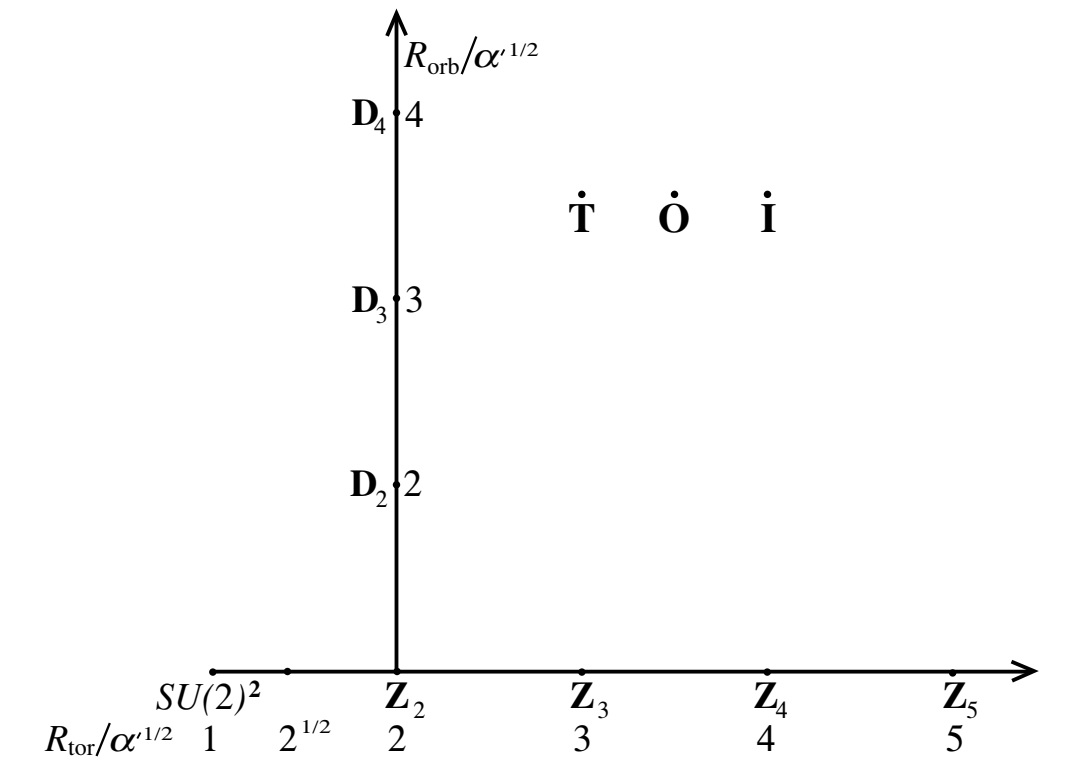
\includegraphics[width=0.8\textwidth]{figure/Fig8.2.jpg}
		\caption{Moduli space of $c=1$ CFT. The horizontal axis is the toroidal branch, while the vertical axis is the orbifold branch. The points marked in the figure are obtained by twisting with a discrete subgroup of the $SU(2)$ group, including three isolated points obtained from the tetrahedral group, the octahedral group, and the icosahedral group.
			Other special radii, such as the torus at $R=(2 \alpha^{\prime})^{1/2}$, will appear later.}\label{Fig8.2}
	\end{center}
\end{figure}

This equivalence holds only at these radii. For example, for a general $R$, toroidal theory only has $U(1) \times U(1)$ gauge symmetry, while the orbifold has no gauge symmetry. 
Therefore, the relationship between the two moduli spaces is as shown in Figure \ref{Fig8.2}. Moduli spaces with different branches meet at special points; in supersymmetric theories, this structure has very general and important features. 
Generally speaking, there will be different low-energy effective theories in each branch, manifested here as low-energy gauge symmetry. More light fields exist near special points. 
As we move away from special points along different branches, different subsets of them become massive.

The low-energy physics near the intersection of the toroidal and orbifold branches is very instructive. Describe it with the $S U(2)$ theory twisted by $r^{\prime}$ in \eqref{8.5.20}. 
The massless scalars remaining under this twisting are $j^{3} \tilde{\jmath}^{3}$ and $j^{i} \tilde{\jmath}^{j}$ for $i, j \in\{1,2\}$. 
Since they are untwisted, the potential is the same as before the twist, i.e., $\mathrm{det} M$. Scalar field $M_{i j}$ can still be diagonalized through $U(1) \times U(1)$ rotations, 
and the potential is flat only when one diagonal element is non-zero. 
However, the modulus $M_{33}$ cannot be rotated to $M_{11}$ or $M_{22}$ now, so these directions are physically different. 
Modulus $M_{33}$ preserves $U(1) \times U(1)$ and corresponds to movement along the toroidal branch. Modulus $M_{11}$ or $M_{22}$ breaks the gauge symmetry and corresponds to movement along the orbifold branch. 
Since this modulus is charged, its sign reversal is a gauge transformation, so physically different orbifolds end at the intersection of branches. We cannot transform two moduli simultaneously because their linear combination is not a flat direction. 
String theory on an orbifold is equivalent to string theory on a circle, which is quite remarkable. This shows that strings perceive spacetime geometry in a way that is not completely identical to ours.

Moving along the toroidal branch, there will be extra massless states at integer multiples of the $SU(2)$ radius $R=k \alpha^{\prime 1/2} $. 
These states have $(n, w)=(\pm 2 k, 0)$. 
We can think of these points as being obtained this way: under $T$-duality, $R=\alpha^{\prime 1/2} / k$, 
they are again obtained by twisting $S U(2) \times S U(2)$ theory using $\mathds{Z}_{k}$ symmetry:
\begin{equation}
	X^{25} \rightarrow X^{25}+\frac{2 \pi \alpha^{\prime 1/2}}{k} \:. \label{8.5.22}
\end{equation}
This multiplies $j^{1}+\mi j^{2}$ and $\tilde{\jmath}^{1}+\mi \tilde{\jmath}^{2}$ by $\exp (2 \pi \mi / k)$ , thus the surviving massless scalars are:
\begin{equation}
	j^{3} \tilde{\jmath}^{3}, \quad j^{1} \tilde{\jmath}^{1}+j^{2} \tilde{\jmath}^{2}, \quad 
	j^{1} \tilde{\jmath}^{2}-j^{2} \tilde{\jmath}^{1} \:. \label{8.5.23}
\end{equation}
The first of these changes the radius of the torus, thus it is always a flat direction. However, because the flatness condition \eqref{8.3.23} for the potential is not met in direction $M_{11}=M_{22}$ or $M_{12}=-M_{21}$, 
no other branches emerge from these points.

Offset \eqref{8.5.22} generates the $\mathds{Z}_{k}$ subgroup of $S U(2) \times S U(2) $. Let us examine twisting with other subgroups. 
Dihedral group $\mathbf{D}_{k}$ consists of offset \eqref{8.5.22} and reflection $X^{25} \rightarrow-X^{25}$, which gives the orbifold at radius $k \alpha^{\prime 1/2}$. 
The other three discrete subgroups are the tetrahedral group, octahedral group, and icosahedral group. They remove all moduli from the CFT, so twisting CFT is an isolated point, not a member of a continuous family. 
Unlike $\mathds{Z}_{k}$ and $\mathbf{D}_{k}$ twisting, which can be defined at all radii, these discrete subgroups containing $S U(2)$ elements exist only at discrete radii, 
thus the radius cannot vary after twisting. String theory with such a compactified space will only have one scalar—the dilaton. 

These are all known $c=1$ CFTs, and thus they give all known 25-dimensional bosonic string backgrounds.

\section{\texorpdfstring{Open Strings}{8.6 Open Strings}} \label{sec:8.6}

In toroidal compactification of open strings, there is a new feature: the possible existence of non-trivial Wilson lines, flat backgrounds for gauge fields. First study some $U(1)$ gauge theories with charged fields, examining constant backgrounds:
\begin{equation}
	A_{25}(x^{M})=-\frac{\theta}{2 \pi R}=-\mi \Lambda^{-1} \frac{\partial \Lambda}{\partial x^{25}}, \quad 
	\Lambda(x^{25})=\exp \biggl(-\frac{\mi \theta x^{25}}{2 \pi R}\biggr) \:, \label{8.6.1}
\end{equation}
where $\theta$ is a constant.
Locally, this is pure gauge, the field strength is zero, and field equations are trivial. However, gauge parameter $\Lambda$ does not satisfy spacetime periodicity, so the background has physical effects. 
The gauge invariant measuring this effect is the Wilson line:
\begin{equation}
	W_{q}=\exp \biggl(\mi q \oint \dif x^{25}\: A_{25}\biggr)=\exp (-\mi q \theta) \:. \label{8.6.2}
\end{equation}

First, consider a point particle with charge $q$; its gauge-fixed action is:
\begin{equation}
	S=\int \dif \tau \: \biggl(\frac{1}{2} \dot{X}^{M} \dot{X}_{M}+\frac{m^{2}}{2}-\mi q A_{M} \dot{X}^{M}\biggr) \:. \label{8.6.3}
\end{equation}
The gauge action is $-\mi q \int \dif x^{M}\, A_{M}$, so a path once around the compact dimension will pick out a phase equal to the Wilson line $W_{q} $. Canonical momentum is:
\begin{equation}
	p_{25}=-\frac{\partial L}{\partial v^{25}}=v^{25}-\frac{q \theta}{2 \pi R} \:, \label{8.6.4}
\end{equation}
where $v^{25}=\mi \dot{X}^{25}$ as in \eqref{8.4.6}.
The wave function must be periodic in the compact dimension, so $p_{25}=l/R$ for integer $l$, and:
\begin{equation}
	v_{25}=\frac{2 \pi l+q \theta}{2 \pi R} \:. \label{8.6.5}
\end{equation}
The Hamiltonian that annihilates physical states is:
\begin{equation}
	H=\frac{1}{2} (p_{\mu} p^{\mu}+v_{25}^{2}+m^{2}) \:, \label{8.6.6}
\end{equation}
since $v_{25}$ depends on $\theta$, $-p_{\mu} p^{\mu}$ is shifted. The same spectrum can be obtained in the field description. 
Note that $v_{25}$ is exactly the gauge-invariant momentum $-\mi \partial_{25}-q A_{25}$. 
We could also perform the gauge transformation $\Lambda^{-1}$ to set $A_{25}$ to zero; under this gauge, the charged field is no longer periodic, 
picking out the phase $\exp (\mi q \theta)$ under $x^{25} \rightarrow x^{25}+2 \pi R$. Physical quantities remain periodic.
The canonical momentum is now shifted, so we have:
\begin{equation}
	v_{25}=p_{25}=\frac{2 \pi l+q \theta}{2 \pi R}\:, \label{8.6.7}
\end{equation}
the same result is obtained for gauge-invariant momentum $v_{25}$ as before.

Now we return to strings and introduce $U(n)$ Chan-Paton factors. 
A general constant $A_{25}$ can be diagonalized by a gauge transformation:
\begin{equation}
	A_{25}=-\frac{1}{2 \pi R} \operatorname{diag}(\theta_{1}, \theta_{2}, \ldots, \theta_{n}) \:. \label{8.6.8}
\end{equation}
This gauge field lies in the diagonal group of $U(n)$, i.e., $U(1)^{n}$. 
The coupling of the gauge field with a general state's Chan-Paton factor is $[A_{M}, \lambda]$, 
so strings in the Chan-Paton state $|i j\rangle$ have charge $+1$ under $U(1)_{i}$, charge $-1$ under $U(1)_{j}$, and are neutral otherwise. Thus it has:
\begin{equation}
	v_{25}=\frac{2 \pi l-\theta_{j}+\theta_{i}}{2 \pi R} \:. \label{8.6.9}
\end{equation}
Then the open string spectrum is:
\begin{equation}
	m^{2}=\frac{(2 \pi l-\theta_{j}+\theta_{i})^{2}}{4 \pi^{2} R^{2}}+\frac{1}{\alpha^{\prime}}(N-1) \:. \label{8.6.10}
\end{equation}

Examine the gauge boson, which has $l=0$ and $N=1$, so:
\begin{equation}
	m^{2}=\frac{(\theta_{j}-\theta_{i})^{2}}{4 \pi^{2} R^{2}} \:. \label{8.6.11}
\end{equation}
In a general background, all $\theta$ are different, and only diagonal vectors with $i=j$ are massless. 
In this case, the unbroken gauge group is $U(1)^{n} $. 
If $r$ of the $\theta$ are equal, the corresponding vector $r \times r$ matrices are massless and carry $U(r)$ gauge symmetry. 
Assigning $n$ of the $\theta$ values to sets $r_{i}$, the gauge symmetry is:
\begin{equation}
	U(r_{1}) \times \ldots \times U(r_{s}), \quad \sum_{i=1}^{s} r_{i}=n \:. \label{8.6.12}
\end{equation}
As before, this has a low-energy interpretation. 
The gauge field $A_{25}$ is a 25-dimensional scalar in the adjoint representation of $U(n)$, and its vacuum expectation value breaks symmetry down to $U(r_{1}) \times \ldots \times U(r_{s})$.

Readers can fill in the details of the low-energy effective action. Note that if there are $k$ compact dimensions, the potential will contain:
\begin{equation}
	\operatorname{Tr}\Bigl([A_{m}, A_{n}]^{2}\Bigr) \:. \label{8.6.13}
\end{equation}
which comes from the field strength in the 26-dimensional Yang-Mills action. This forces gauge fields in different directions to commute in static solutions, allowing them to be simultaneously diagonalized. There are $kn$ moduli from gauge fields, and $k^{2}$ moduli from the metric and antisymmetric tensor.

\subsection*{$T$-duality}

Now examine the $R \rightarrow 0$ limit of the open string spectrum. If open string boundaries are Neumann boundaries, there is no quantum number analogous to $w$; they can always be untied from compact dimensions. 
So, as $R \rightarrow 0$, states with non-zero momentum acquire infinite mass, but there are no new continuous states. 
This is consistent with field theory behavior: corresponding states move in 25 spacetime dimensions.

We know that theories with open strings must have closed strings, which seems to cause a contradiction. It makes closed strings move in 26 spacetime dimensions while open strings move in 25 spacetime dimensions in the $R \rightarrow 0$ limit. 
From this it can be inferred that: the interior of an open string is identical to a closed string, composed of the same "matter", so it still vibrates in 26 dimensions. What distinguishes open strings is exactly their endpoints, 
so they must be restricted to a 25-dimensional hyperplane. 
Indeed, we can use new embedding coordinates to describe the $T$-duality theory:
\begin{equation}
	X^{\prime 25}(z, \bar{z})=X_{L}^{25}(z)-X_{R}^{25}(\bar{z}) \:. \label{8.6.14}
\end{equation}
Then:
\begin{equation}
	\partial_{n} X^{25}=-\mi \partial_{t} X^{\prime 25} \:, \label{8.6.15}
\end{equation}
where $n$ is the normal direction to the boundary, and $t$ is the tangent direction to the boundary. 
Neumann boundaries in the original coordinates become Dirichlet boundaries in the dual coordinates: the $X^{\prime 25}$ coordinate of each string endpoint is fixed. 

Let us first examine compactification without Wilson lines. Then all endpoints are constrained to the same hyperplane. To see this, integrate:
\begin{align}
	X^{\prime 25}(\pi)-X^{\prime 25}(0) &= \int_{0}^{\pi} \dif \sigma^{1}\: \partial_{1} X^{\prime 25}
	= -\mi \int_{0}^{\pi} \dif \sigma^{1}\: \partial_{2} X^{25} \nonumber \\
	&= -2 \pi \alpha^{\prime} v^{25}
	= -\frac{2 \pi \alpha^{\prime} l}{R}=-2 \pi l R^{\prime} \:. \label{8.6.16}
\end{align}
The total change of $X^{\prime 25}$ between two endpoints is an integer multiple of the dual dimension period $2 \pi R^{\prime}$, so the endpoints lie on the same hyperplane in the periodic $T$-dual space. 
For two different open strings, exchanging a graviton between them yields a connected worldsheet. We can apply the same argument as in \eqref{8.6.16} to this, so all string endpoints lie on the same hyperplane, 
as seen in Figure \ref{Fig8.3}. Endpoints move freely in the other 24 dimensions.

\begin{figure}[!htbp]
	\begin{center}
		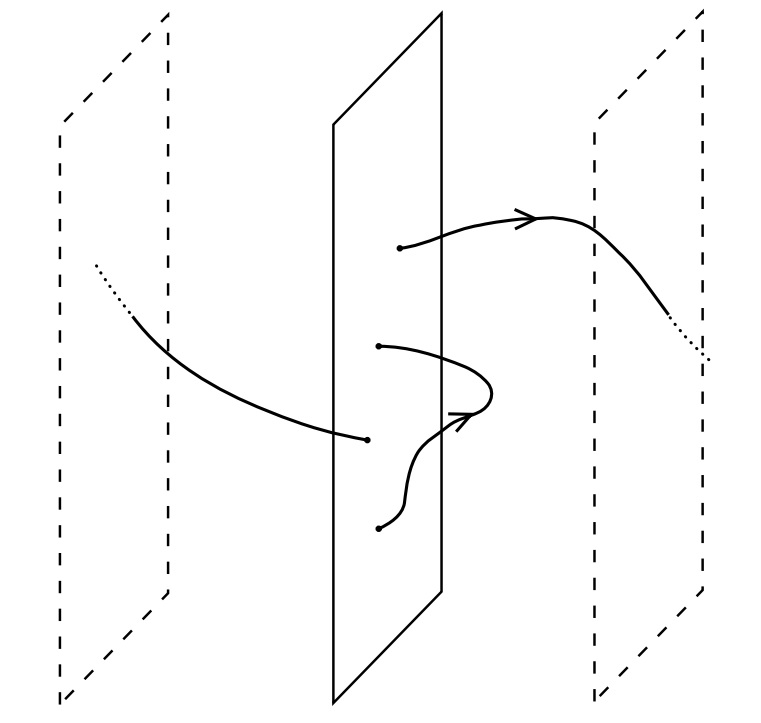
\includegraphics[width=0.7\textwidth]{figure/Fig8.3.jpg}
		\caption{Open strings with endpoints attached to a hyperplane. The planes marked with dashed lines are periodically equivalent planes. Two strings are shown in the figure, with winding numbers 1 and 0 respectively.}\label{Fig8.3}
	\end{center}
\end{figure}

Now let us look at the effect of Wilson lines. 
Due to the shift in $v_{25}$ in \eqref{8.6.9}, \eqref{8.6.16} is replaced by:
\begin{equation}
	\Delta X^{\prime 25}=X^{\prime 25}(\pi)-X^{\prime 25}(0)=-(2 \pi l-\theta_{j}+\theta_{i}) R^{\prime} \:. \label{8.6.17}
\end{equation}
In other words, discarding an extra normalization, endpoints on state $i$ are at:
\begin{equation}
	X^{\prime 25}=\theta_{i} R^{\prime}=-2 \pi \alpha^{\prime} A_{25, i i} \:. \label{8.6.18}
\end{equation}
Thus, there are generally $n$ different hyperplanes, as seen in Figure \ref{Fig8.4}.

\begin{figure}[!htbp]
	\begin{center}
		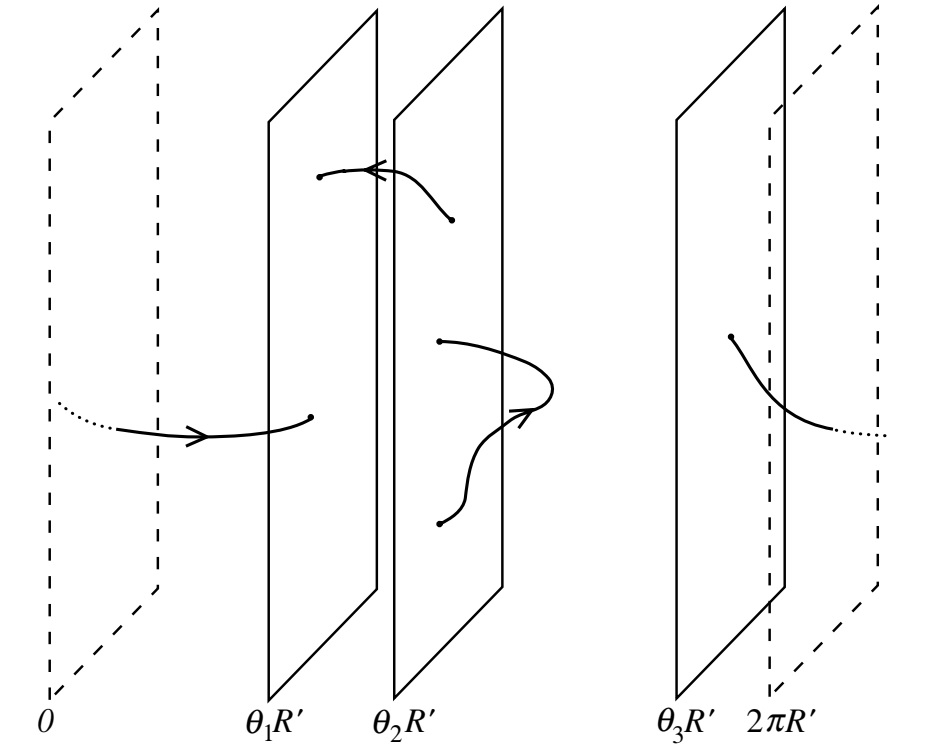
\includegraphics[width=0.8\textwidth]{figure/Fig8.4.jpg}
		\caption{$n=3$ hyperplanes at different positions, with different strings attached. Ignoring tachyons, the lightest strings with both ends on the same hyperplane are massless, while strings connecting two non-coincident hyperplanes are massive due to tension. When two hyperplanes coincide, the lightest strings connecting them become massless.}\label{Fig8.4}
	\end{center}
\end{figure}

Let us examine the mode expansion for the Chan-Paton state $|i j\rangle$, assuming it winds $l$ times around the compact dimension:
\begin{align}
	X^{\prime 25}(z, \bar{z}) &= \theta_{i} R^{\prime} - \frac{\mi R^{\prime}}{2 \pi}(2 \pi l-\theta_{j}+\theta_{i}) 
	\ln (z / \bar{z}) + \mi \biggl(\frac{\alpha^{\prime}}{2}\biggr)^{1/2} 
	\sum_{m=-\infty \atop m \neq 0}^{\infty} \frac{\alpha_{m}^{25}}{m}(z^{-m}-\bar{z}^{-m})  \nonumber \\
	&=\theta_{i} R^{\prime} + \frac{\sigma^{1}}{\pi} \Delta X^{\prime 25} - (2 \alpha^{\prime})^{1/2} 
	\sum_{m=-\infty \atop m \neq 0}^{\infty} \frac{\alpha_{m}^{25}}{m} \exp (-m \sigma^{2}) \sin m \sigma^{1} \:. \label{8.6.19}
\end{align}
The spectrum \eqref{8.6.10} becomes:
\begin{equation}
	m^{2}=\biggl(\frac{\Delta X^{\prime 25}}{2 \pi \alpha^{\prime}}\biggr)^{2}+\frac{1}{\alpha^{\prime}}(N-1) \:, \label{8.6.20}
\end{equation}
where $\Delta X^{\prime 25}$ is given by \eqref{8.6.17}. It is the shortest length of a string in a given sector.

Now examine how this picture generalizes if there are multiple compact dimensions. 
Let $X^{m}$ be periodic dimensions, where $p+1 \leq m \leq 25$. We write periodic dimensions in the form of dual coordinates. 
Neumann conditions on $X^{m}$ again become Dirichlet conditions on dual coordinates $X^{\prime m}$, so open string endpoints are restricted to $n$ parallel $(p+1)$-dimensional subspaces. 
For each subspace, Wilson lines in different directions become independent coordinates. 
Since translation invariance is broken by open string boundary conditions, the dual background is quite strange. This reflects the fact that: in the original open string theory, winding number is not conserved, and winding number $T$-duals to momentum. 
$T$-duality is just a different description of the same theory. Furthermore, when the compactification radius is very small, the $T$-duality picture should naturally be used.

\section{\texorpdfstring{D-branes}{8.7 D-branes}} \label{sec:8.7}
We now know that when an open string theory is compactified on a small torus, its physics can be described as compactification on a large torus, but with open string endpoints constrained to subspaces. In fact, these subspaces themselves are new dynamical objects. 
Consider the spectrum of massless open strings in a general configuration, where all $\theta_{i}$ are different, and for simplicity, only one coordinate is dualized. 
Ignoring tachyons, mass \eqref{8.6.20} is only zero when $N=1$ and $\Delta X^{\prime 25}=0 $. That is, both endpoints are on the same hyperplane and the winding number is zero. Thus we have massless states:
\begin{subequations} \label{8.7.1}
	\begin{align}
		&\alpha_{-1}^{\mu}|k; ii\rangle \:, \quad \mathscr{V} = \mi \partial_{t} X^{\mu}  \:, \label{8.7.1a} \\
		&\alpha_{-1}^{25} |k; ii\rangle \:, \quad \mathscr{V} = \mi \partial_{t} X^{25} = \partial_{n} X^{\prime 25} \:. \label{8.7.1b}
	\end{align}
\end{subequations}
They are obviously massless states in the original theory; $T$-duality just provides a different view of the same spectrum. For general Wilson lines, the only massless open string states will be $n$ massless $U(1)$ vectors. 
In \eqref{8.7.1}, we classified them according to whether they are tangent or normal to the hyperplane. 
The 25 states with tangential polarizations constitute a gauge field on the hyperplane, 
which has a simple and important interpretation in the $T$-duality theory: it is a set of coordinates for the shape of the hyperplane. This can be seen from the fact that a constant gauge field \eqref{8.6.18} corresponds to a uniform translation of the hyperplane. 
A background depending on $x^{\mu}$ can shift to a translation depending on $x^{\mu}$, a curved hyperplane, and the quantum of field $A_{ii}^{25}$ corresponds to a small oscillation of the hyperplane.

This is identical to phenomena occurring in spacetime. We start with strings in a flat background and discover that massless closed string states correspond to fluctuations in geometry. 
Here, we first discover hyperplanes, and then discover that specific open string states correspond to fluctuations of the hyperplanes. We should not be surprised that hyperplanes have dynamics. 
String theory includes gravity. Gravitational waves passing through a hyperplane will perturb spacetime itself, so it is difficult for hyperplanes to remain rigid. 
Thus, hyperplanes are indeed dynamical objects; these are D-branes. Performing duality on $25-p$ dimensions results in $p$-dimensional branes, called D$p$-branes. 
Using this terminology, the original $U(n)$ open string theory contains $n$ D25-branes. D25-branes fill the space, so there are no constraints on string endpoints: it just corresponds to general Chan-Paton factors. 
Since $T$-duality swaps Neumann and Dirichlet boundary conditions, $T$-duality in a direction tangent to a D$p$-brane reduces it to a D$(p{-}1)$-brane, 
while $T$-duality in a normal direction reduces it to a D$(p{+}1)$-brane. Non-trivial angle cases appear immediately. 

We could have started by studying Dirichlet boundaries themselves. Here the route we took was discovering them from $T$-duality, a method that better develops their properties. 
It can also be proven that through a continuous process, we can move from "ordinary" states to states containing D-branes. That is, taking the $R \rightarrow 0$ limit of the ordinary theory, which results in $n$ D-branes in non-compact space. 
In superstrings, we will use this to argue that D-branes are an important part of the non-perturbative definition of the theory. For bosonic strings, since there is no strong evidence that it has a non-perturbative definition, we do not discuss this. 
Bosonic string theory possibly exists only as a part of superstrings.

Let us look at $U(n)$ symmetry breaking in the $T$-duality picture. When no D-branes coincide, there are massless vectors only on each D-brane, yielding the gauge group $U(1)^{n}$. 
If $r$ D-branes coincide, there will be extra massless states, with the length of the strings connecting these branes being zero: when $n=0$, if both $i$ and $j$ are in set $r$, 
$\Delta X^{\prime 25}$ in mass formula \eqref{8.6.20} is zero. Thus, there are $r^{2}$ vectors, forming the adjoint representation of the $U(r)$ gauge group. 
This is the same as discovered in the dual Wilson line picture. However, surprisingly, there will be $r^{2}$ massless scalars in directions normal to the D-branes. We will discuss its meaning below.

\subsection*{D-brane Action}
On the worldvolume of a D$p$-brane, the massless fields are $U(1)$ vectors and $25{-}p$ worldvolume scalars describing fluctuations. The low-energy effective action for this system is always worth examining. 
We take the dual radius $R^{\prime}$ to be infinite and only consider a single D-brane in the corresponding 26-dimensional spacetime. Worldvolume fields interact with massless closed string fields, and its action was discussed in section \ref{sec:3.7}. 
Introduce coordinates $\xi^{a}$ on the brane, where $a=0, \ldots p$. Fields on the brane are the embedding $X^{\mu}(\xi)$ and the gauge field $A_{a}(\xi)$. 
We declare the action to be:
\begin{equation}
	\bm{S}_{p} = -T_{p} \int \dif^{p+1} \xi \: 
	\me^{-\Phi}[-\operatorname{det}(G_{ab} + B_{ab} + 2 \pi \alpha^{\prime} F_{a b})]^{1/2} \:, \label{8.7.2}
\end{equation}
\begin{tcolorbox}
	\begin{remark}
		We not know the full D-brane action in closed form. Above is low energy Effective Action.
	\end{remark}
\end{tcolorbox}
where $T_{p}$ is a constant to be determined. 
Here:
\begin{equation}
	G_{ab}(\xi) = \frac{\partial X^{\mu}}{\partial \xi^{a}} \frac{\partial X^{\nu}}{\partial \xi^{b}} G_{\mu \nu}(X(\xi)), \quad 
	B_{ab}(\xi) = \frac{\partial X^{\mu}}{\partial \xi^{a}} \frac{\partial X^{\nu}}{\partial \xi^{b}} B_{\mu \nu}(X(\xi)) \label{8.7.3}
\end{equation}
are the induced metric and induced antisymmetric tensor on the brane. 
All features of \eqref{8.7.2} can be understood based on general reasoning. First, considering only the spacetime metric and embedding, 
the simplest coordinate-independent action with fewest derivatives is the integral of $(-\operatorname{det} G_{a b})^{1/2}$, i.e., the worldvolume. 
Note that this term has an implicit relationship to $X^{\mu}(\xi)$ via the induced fields \eqref{8.7.3}. Expanding around a flat D-brane gives the action for fluctuations, 
just as the Nambu-Goto action describes string fluctuations.
\begin{tcolorbox}[breakable]
			A D$p$-brane is defined as a $p+1$ dimensional hyperplane in a $D$-dimensional spacetime to which open string endpoints are attached. These hyperplanes arise when Dirichlet boundary conditions are imposed in transverse directions, replacing the standard Neumann boundary conditions. 
			
				Dirichlet boundary conditions also arise through the T-duality of a compactified dimension with Neumann conditions. Specifically, the string satisfies Neumann boundary conditions in the directions along the hyperplane:
				\begin{equation}
					\frac{\partial X^\mu}{\partial \sigma} \Big|_{\sigma=0,\pi} = 0 \quad \text{for } \mu = 0, 1, \dots, p 
				\end{equation}
				and Dirichlet boundary conditions in the transverse directions:
				\begin{equation}
					X^\mu \Big|_{\sigma=0,\pi} = 0 \quad \text{for } \mu = p+1, \dots, D
				\end{equation}
				The endpoints of the open string in the original theory,
				\[
				X^\mu = X_L^\mu + X_R^\mu, \qquad \mu = 0, \ldots, D,
				\]
				are not fixed and satisfy Neumann boundary conditions. 
				However, the dual coordinates satisfy Dirichlet boundary conditions, and their endpoints are fixed on the D$p$-branes. The position of the D-brane is fixed by the dual coordinates $X'^{p+1}, \dots, X'^D$ defined in \eqref{8.6.18} such that:
				\begin{equation}
					X'^k = -2\pi \alpha' A_{k,ii} \quad \text{for } k = p+1, \dots, D
				\end{equation}
				where $i$ is the Chan-Paton index, linking the endpoints to a specific background $A_k$. For a single compactified dimension with $U(N)$ Chan-Paton factors, we consider an Abelian gauge background:
				\begin{equation}
					A_d = \frac{1}{2\pi R} \begin{pmatrix} \theta_1 & 0 & \dots & 0 \\ 0 & \theta_2 & \dots & 0 \\ \dots & \dots & \dots & \dots \\ 0 & 0 & \dots & \theta_N \end{pmatrix} 
				\end{equation}
				This field is pure gauge, $A_d = -i \Lambda^{-1} \partial_d \Lambda$, with:
				\begin{equation}
					\Lambda = \text{diag}(e^{i\theta_1 X^d / 2\pi R}, e^{i\theta_2 X^d / 2\pi R}, \dots, e^{i\theta_N X^d / 2\pi R}) 
				\end{equation}
				Although $A_d$ can be gauged away locally to zero via $\Omega(X) = \text{diag}(-\frac{\theta_1}{2\pi R}, \dots, -\frac{\theta_N}{2\pi R})$, it cannot be gauged away globally because $\Lambda(X)$ is not periodic:
				\begin{equation}
					\Lambda(X^d + 2\pi R) = \text{diag}(e^{i\theta_1}, \dots, e^{i\theta_N}) \Lambda(X^d) = W \cdot \Lambda(X^d) 
				\end{equation}
				The gauge invariant observable is the Wilson line $W = e^{i \oint dx^d A_d}$. Gauge invariant states pick up a phase after a periodic translation $X^d \to X^d + 2\pi R$, resulting in $U(N)$ symmetry breaking into $[U(1)]^N$. For a state $|k; ij\rangle$, endpoint $i$ picks up phase $e^{-i\theta_i / 2\pi R}$ and endpoint $j$ picks up $e^{-i\theta_j / 2\pi R}$, resulting in the wave function transformation:
				\begin{equation}
					|k; ij\rangle \to e^{i(\theta_j - \theta_i) / 2\pi R} |k; ij\rangle 
				\end{equation}
				This quantizes the momentum of that state as:
				\begin{equation}
					p_{(ij)}^D = \frac{n}{R} + \frac{\theta_j - \theta_i}{2\pi R} 
				\end{equation}
				The dual coordinates $X'^D$ then have endpoints fixed on hyperplanes at:
				\begin{equation}
					X'^D(\sigma=0; i) = 2\pi \alpha' A_{ii}^D \quad \text{and} \quad X'^D(\sigma=\pi; j) = 2\pi \alpha' A_{jj}^D 
				\end{equation}
				
				For multiple compactified dimensions, the mass spectrum generalizes to:
				\begin{equation}
					m^2 = \sum_{k=p+1}^D \left( \frac{\Delta X'^k}{2\pi \alpha'} \right)^2 + \frac{N - 1}{\alpha'} 
				\end{equation}
				Substituting the dual coordinates difference:
				\begin{equation}
					m^2 = \sum_{k=p+1}^D \left( \frac{2\pi l^k - \theta_i + \theta_j}{2\pi \alpha'} \right)^2 + \frac{N - 1}{\alpha'} 
				\end{equation}
				If $k$ endpoints have identical values ($\theta_1 = \dots = \theta_k = \theta$), massless states exist for $l^k = 0$ and $N=1$ even for strings stretched between different hyperplanes, as these hyperplanes are located at the same place. There are $k^2$ such massless states transforming under the adjoint representation of $U(k)$. This results in an unbroken $U(k)$ symmetry, providing a gauge theory on the D$p$-brane with scalar fields $\Phi_{ij}^m(\xi^a)$ describing D-brane dynamics.
			
			The derivation of the low-energy action starts with a free open string coupled to a constant background field strength $F_{\mu\nu} = \partial_\mu A_\nu - \partial_\nu A_\mu$. We have seen that we can also view this as a theory of open strings with end-points on a $D-$brane of dimension D, the entire	space-time. 
			
			Our goal is to work out a tree-level scattering amplitude using perturbation theory. We	are thus interested in a disc diagram with insertions at the boundary, or via a conformal	transformation a unit circle with four insertions on the boundary. We utilize the unit disc with polar coordinates $z = re^{i\theta}$ and the Green's function/kernel $f(z, z')$ with Neumann boundary conditions:
			\begin{equation}
				\partial \bar{\partial} f(z, z') = \delta(z - z') \quad \text{and} \quad \partial_r f(z, z') \big|_{r=1} = 0 
			\end{equation}
			The solution is:
			\begin{equation}
				f(z, z') = \frac{1}{2\pi} (\ln |z - z'| + \ln |z - \bar{z}'^{-1}|) 
			\end{equation}
			On the boundary ($r=1$), where $z' = \bar{z}'^{-1} = e^{i\theta}$ and $\bar{z}' = z'^{-1} = e^{-i\theta}$, this becomes:
			\begin{equation}
				f(\theta, \theta') = \frac{1}{2\pi} \ln (e^{i\theta} - e^{i\theta'})(e^{-i\theta} - e^{-i\theta'}) = \frac{1}{2\pi} \ln [2 - 2 \cos(\theta - \theta')] 
			\end{equation}
			Using the series expansion $\ln(1 + b^2 - 2b \cos x) = -2 \sum_{m=1}^\infty \frac{b^m}{m} \cos mx$ for $b=1$, we find:
			\begin{equation}
				f(\theta, \theta') = -\frac{1}{\pi} \sum_{n=1}^\infty \frac{1}{n} \cos n(\theta - \theta')\label{8.511} 
			\end{equation}
			We can alternatively prove this by expanding the logarithms:
			\begin{align}
				f(\theta, \theta') &= \frac{1}{2\pi} [ \ln e^{i\theta} + \ln(1 - e^{i\theta' - \theta}) + \ln e^{-i\theta} + \ln(1 - e^{-i\theta' - \theta}) ] \notag\\
				&= -\frac{1}{2\pi} \left[ \sum_{n=1}^\infty \frac{e^{in(\theta - \theta')}}{n} + \sum_{n=1}^\infty \frac{e^{-in(\theta - \theta')}}{n} \right] = -\frac{1}{\pi} \sum_{n=1}^\infty \frac{\cos [n(\theta - \theta')]}{n} 
			\end{align}
			The inverse Green's function $f^{-1}(\theta, \theta')$ must satisfy $\int d\theta' f(\theta, \theta') f^{-1}(\theta', \theta'') = \delta(\theta - \theta'') - \frac{1}{2\pi}$. It is given by:
			\begin{equation}
				f^{-1}(\theta, \theta') = -\frac{1}{\pi} \sum_{n=1}^\infty n \cos n(\theta - \theta') \label{8.513}
			\end{equation}
			To check this, evaluate the integral:
			\begin{equation}
				\int_0^{2\pi} d\theta' f(\theta, \theta') f^{-1}(\theta', \theta'') = \frac{1}{\pi^2} \int_0^{2\pi} d\theta' \sum_{m,n=1}^\infty \frac{m}{n} \cos [n(\theta - \theta')] \cos [m(\theta' - \theta'')] 
			\end{equation}
			Using $\cos n(\theta - \theta') = \cos n\theta \cos n\theta' + \sin n\theta \sin n\theta'$ and the orthogonality relations $\int_0^{2\pi} d\theta' \cos m\theta' \cos n\theta' = \int_0^{2\pi} d\theta' \sin m\theta' \sin n\theta' = \pi \delta_{m,n}$:
			\begin{equation}
				= \frac{1}{\pi} \sum_{m=1}^\infty ( \cos m\theta \cos m\theta'' + \sin m\theta \sin m\theta'' ) = \frac{1}{\pi} \sum_{m=1}^\infty \cos m(\theta - \theta'') 
			\end{equation}
			With the Fourier decomposition $\frac{1}{\pi} \sum_{m=1}^\infty \cos m(\theta - \theta'') = \delta(\theta - \theta'') - \frac{1}{2\pi}$, the following is satisfied:
			\begin{equation}
				\int_0^{2\pi} d\theta' f(\theta, \theta') f^{-1}(\theta', \theta'')=\delta(\theta-\theta')-\frac{1}{2\pi}\label{8.519}
			\end{equation}
			
			\begin{proof}	
			The bosonic string coupled to a photon field in the conformal gauge has action:
			\begin{equation}
				S[X, A] = \frac{1}{4\pi\alpha'} \int d^2z \partial X^\mu \bar{\partial} X_\mu - i \oint d\theta \partial_\theta A_\mu \big|_{r=1} 
			\end{equation}
			Note that the contribution of the minimally coupled photon field can be seen to correspond
			to the insertion of an open string vertex operator. As we integrate out the spacetime fields
			$X^{\mu}$ the resulting partition function is a functional of the gauge field only, and because of gauge invariance of the Wilson loop it must be a functional of the field strength $F_{\mu\nu}$. We evaluate the Euclidean path integral $Z[F] = \frac{1}{g_s} \int \mathcal{D}X^\mu e^{-S}$ using the background method $X^\mu = X_0^\mu + \xi^\mu$. In the radial gauge $\xi^\mu A_\mu(X_0 + \xi) = 0$ and assuming constant $F_{\mu\nu}$, the path integral measure $\mathcal{D}X^\mu$ is split between the interior and the boundary:
			\begin{equation}
				\mathcal{D}X^\mu = \prod_{|z|<1} \mathcal{D}X^\mu(z, \bar{z}) \prod_{boundary} \mathcal{D}\xi^\mu(\theta) 
			\end{equation}
			Reducing the interior integration to a boundary integral by introducing field $\eta(\theta)$ and representing the delta function $\delta^{(D)}(\xi^\mu - \eta^\mu)$ as a Gaussian over auxiliary fields $\nu^\mu$:
			\begin{align*}
				Z[F] &= \int \mathcal{D}\xi^\mu e^{-\frac{1}{4\pi\alpha'} \int d\theta \partial \xi^\mu \bar{\partial} \xi_\mu} \int \mathcal{D}\eta^\mu \delta^{(D)}(\xi^\mu - \eta^\mu) \times \text{o.c.} \\
				&= \int \mathcal{D}\xi^\mu \mathcal{D}\eta^\mu e^{-\frac{1}{4\pi\alpha'} \int d\theta \partial \xi^\mu \bar{\partial} \xi_\mu} \frac{1}{(2\pi)^D} \int \mathcal{D}\nu^\mu e^{i \int d\theta \nu^\mu (\xi_\mu - \eta_\mu)} \times \text{o.c.} \\
				&= \frac{1}{(2\pi)^D} \int \mathcal{D}\eta^\mu \mathcal{D}\nu^\mu \int \mathcal{D}\xi^\mu e^{\int d\theta \left[ -\frac{1}{4\pi\alpha'} \partial \xi^\mu \bar{\partial} \xi_\mu + i \nu^\mu (\xi_\mu - \eta_\mu) \right]} \times \text{o.c.}
			\end{align*}
			where o.c. stands for other contributions. Rescaling $\xi$ and $\eta$ by $\sqrt{2\pi \alpha'}$ and performing Gaussian integrations:
			\begin{align*}
				Z[F] &\propto \int \mathcal{D}\eta^\mu \mathcal{D}\nu^\mu \int \mathcal{D}\xi^\mu e^{-\xi^\mu \left( -\frac{\partial\bar{\partial}}{2} \right) \xi_\mu + i \sqrt{2\pi\alpha'} \nu^\mu (\xi_\mu - \eta_\mu)} \times \text{o.c.} \\
				&\propto \int \mathcal{D}\eta^\mu \mathcal{D}\nu^\mu \left( \frac{\pi}{\text{det}(-\partial\bar{\partial}/2)} \right)^{\frac{D}{2}} e^{-\nu^\mu \frac{4\pi\alpha'}{\partial\bar{\partial}} \nu_\mu - i \sqrt{2\pi\alpha'} \nu^\mu \eta_\mu} \times \text{o.c.} \\
				&\propto \int \mathcal{D}\eta^\mu \left( \frac{\pi}{\text{det}(-\partial\bar{\partial}/2)} \right)^{\frac{D}{2}} \left( \frac{\pi}{\text{det}(4\pi\alpha'/\partial\bar{\partial})} \right)^{\frac{D}{2}} e^{-\frac{2\pi\alpha'\eta^\mu\eta_\mu}{4\pi\alpha'/\partial\bar{\partial}}} \times \text{o.c.} \\
				&\propto \int \mathcal{D}\eta^\mu e^{-\eta^\mu \frac{\partial\bar{\partial}}{2} \eta_\mu} \times \text{o.c.}
			\end{align*}
			Renaming $\eta$ to $\xi$, the kinetic term contribution is $\int \mathcal{D}\xi^\mu e^{-\frac{1}{2} \xi^\mu f^{-1} \xi_\mu}$. The gauge field term rescales by $2\pi\alpha'$, becoming:
			\begin{equation}
				i \int_0^{2\pi} d\theta F_{\mu\nu} \xi^\mu \dot{\xi}^\nu = \frac{i}{2} \int_0^{2\pi} d\theta ( \partial_\mu A_\nu \xi^\mu \dot{\xi}^\nu - \partial_\mu A_\nu \xi^\nu \dot{\xi}^\mu ) = i \int_0^{2\pi} d\theta \partial_\mu A_\nu \xi^\mu \dot{\xi}^\nu + o(\partial F) 
			\end{equation}
			Combining these gives the boundary path integral:
			\begin{equation}
				Z[F] \propto \int \mathcal{D}\xi^\mu \exp \left( -\frac{1}{2} \xi^\mu f^{-1} \xi_\mu + \frac{i}{2} F_{\mu\nu} \int_0^{2\pi} d\theta \xi^\mu \dot{\xi}^\nu \right) 
			\end{equation}
			Using Lorentz invariance, we bring the antisymmetric matrix $F_{\mu\nu}$ into its Jordan normal form, consisting of $D/2$ antisymmetric $2 \times 2$ blocks:
			\begin{equation}
				F_{\mu\nu} = \begin{pmatrix} 
					0 & -f_1 & & 0 & 0 \\
					f_1 & 0 & & 0 & 0 \\
					& & \ddots & & \\
					0 & 0 & & 0 & -f_{D/2} \\
					0 & 0 & & f_{D/2} & 0 
				\end{pmatrix}
			\end{equation}
			
			Substituting this into the interaction term, we expand the product $\xi^\mu F_{\mu\nu} \dot{\xi}^\nu$:
			\begin{align}
				\xi^\mu F_{\mu\nu} \dot{\xi}^\nu &= (\xi^1 \ \dots \ \xi^D) \begin{pmatrix} 
					0 & -f_1 & & 0 & 0 \\
					f_1 & 0 & & 0 & 0 \\
					& & \ddots & & \\
					0 & 0 & & 0 & -f_{D/2} \\
					0 & 0 & & f_{D/2} & 0 
				\end{pmatrix} \begin{pmatrix} \dot{\xi}^1 \\ \vdots \\ \dot{\xi}^D \end{pmatrix} \\
				&= -\xi^1 \dot{\xi}^2 f_1 + \xi^2 \dot{\xi}^1 f_1 - \xi^3 \dot{\xi}^4 f_2 + \xi^4 \dot{\xi}^3 f_2 + \dots - \xi^{D-1} \dot{\xi}^D f_{D/2} + \xi^D \dot{\xi}^{D-1} f_{D/2} \\
				&= \sum_{k=1}^{D/2} \left( -\xi^{2k-1} \dot{\xi}^{2k} + \xi^{2k} \dot{\xi}^{2k-1} \right) f_k 
			\end{align}
			
			The path integral factorizes into $D/2$ independent $2 \times 2$ blocks. Applying partial integration to the second term in the sum for each block:
			\begin{equation}
				Z[F] \propto \prod_{k=1}^{D/2} \int \mathcal{D}\xi^{2k-1} \mathcal{D}\xi^{2k} \exp \left[ -\left( \frac{1}{2} \xi^{2k-1} f^{-1} \xi^{2k-1} + \frac{1}{2} \xi^{2k} f^{-1} \xi^{2k} + i f_k \xi^{2k-1} \dot{\xi}^{2k} \right) \right]
			\end{equation}
			
			We integrate over $\xi^{2k}$ using the Gaussian functional identity $\int \mathcal{D}x e^{-\frac{1}{2} x A x + Jx} \propto (\det A)^{-1/2} e^{\frac{1}{2} J A^{-1} J}$. Renaming $\xi^{2k-1}$ as $\xi$:
			\begin{align}
				Z[F] &\propto \prod_{k=1}^{D/2} \int \mathcal{D}\xi \sqrt{\frac{2\pi}{\det(f^{-1})}} \exp \left( -\frac{1}{2} \xi f^{-1} \xi - \frac{f_k^2 \dot{\xi} \dot{\xi}}{4 f^{-1}/2} \right) \\
				&\propto \prod_{k=1}^{D/2} \int \mathcal{D}\xi \sqrt{2\pi \det(f)} \exp \left( -\frac{1}{2} \xi f^{-1} \xi - \frac{1}{2} f_k^2 \dot{\xi} f \dot{\xi} \right) \\
				&\propto \prod_{k=1}^{D/2} \int \mathcal{D}\xi \sqrt{2\pi \det(f)} \exp \left[ -\frac{1}{2} \xi \left( f^{-1} + f_k^2 \ddot{f} \right) \xi \right]
			\end{align}
			where we have defined $\ddot{f}(\theta, \theta') = \partial_\theta \partial_{\theta'} f(\theta, \theta')$ through partial integration. The final integration over the remaining coordinates $\xi$ yields:
			\begin{equation}
				Z[F] \propto \prod_{k=1}^{D/2} \sqrt{2\pi \det(f)} \sqrt{\frac{2\pi}{\det(f^{-1} + f_k^2 \ddot{f})}} \propto \prod_{k=1}^{D/2} \left[ \det(f^{-1}f + f_k^2 \ddot{f} f) \right]^{-1/2}
			\end{equation}
			Rescaling the tensor $F_{\mu\nu} \to 2\pi\alpha' F_{\mu\nu}$, we have
			\begin{equation}
				Z[F] = Z[0] \prod_{k=1}^{D/2} (\det \Delta_k)^{-1/2} \quad \text{with} \quad \Delta_k = f^{-1}f + (2\pi\alpha' f_k)^2 \ddot{f} f\label{8.538}
			\end{equation}
			To proceed we need to compute $f \ddot{f}$, which can be done by using the integral kernels \eqref{8.511} and $\ddot{f} = \partial_\theta \partial_{\theta'} f(\theta, \theta')$,
			\begin{equation}
				\dot{f} = \frac{1}{\pi} \sum_{n=1}^{\infty} \sin n(\theta - \theta') \quad \text{and} \quad \ddot{f} = -\frac{1}{\pi} \sum_{n=1}^{\infty} n \cos n(\theta - \theta')
			\end{equation}
			
			From \eqref{8.513} we see that $\ddot{f} = f^{-1}$ and therefore $\ddot{f} f = f^{-1} f = \delta(\theta - \theta') - \frac{1}{2\pi} = \bar{\delta}(\theta - \theta')$, where we have used \eqref{8.519}. We therefore get the following kernel form of the $\Delta_k$ operator:
			\begin{equation}
				\Delta_k(\theta, \theta') = [1+ (2\pi\alpha' f_k)^2] \bar{\delta}(\theta - \theta')
			\end{equation}
			To evaluate the determinant of this operator, we expand any field in the orthonormal basis on the boundary of the disk. The basis elements are $E_m = \pi^{-1/2} \cos m\theta$ and $F_m = \pi^{-1/2} \sin m\theta$ for $m \ge 1$. For any basis element $E_n$, the action of the $\bar{\delta}(\theta - \theta')$ operator is:
			\begin{align}
				\int_0^{2\pi} d\theta' \bar{\delta}(\theta - \theta') E_n(\theta') &= \int_0^{2\pi} d\theta' \delta(\theta - \theta') E_n(\theta') -\underbrace{ \frac{1}{2\pi} \int_0^{2\pi} E_n(\theta') d\theta'}_{=0 \text{ for $n\ge1$}}\notag\\
				&=E_n(\theta)
			\end{align}
			As a result, the basis elements $E_n$ and $F_n$ are thus eigenfunctions of $\Delta_k$ with eigenvalues:
			\begin{equation}
			\int_0^{2\pi} \Delta_k(\theta, \theta') E_m(\theta') d\theta' = E_m(\theta) + (2\pi\alpha' f_k)^2 E_m(\theta) = [1 + (2\pi\alpha' f_k)^2] E_m(\theta)
			\end{equation}
			Because each $n$ corresponds to two degenerate eigenfunctions ($E_n$ and $F_n$), the determinant over the fluctuation space is the infinite product:
			\begin{equation}
				\det \Delta_k = \prod_{n=1}^{\infty} [1 + (2\pi\alpha' f_k)^2]^2
			\end{equation}
			Plugging this in \eqref{8.538} we find that
			\begin{equation}
				Z[F] = Z[0] \prod_{k=1}^{D/2} (\det \Delta_k)^{-1/2} = Z[0] \prod_{k=1}^{D/2} \prod_{m=1}^{\infty} [1 + (2\pi\alpha' f_k)^2]^{-1}
			\end{equation}
			Regularizing via the Riemann zeta function $\zeta(s) = \sum n^{-s}$ where $\zeta(0) = -1/2$:
			\begin{equation}
				\prod_{m=1}^\infty c^{-1} = e^{ - \zeta(0) \ln c } = c^{1/2} 
			\end{equation}
			Which results in
			\begin{equation}
				Z[F]= Z[0] \prod_{k=1}^{D/2} \prod_{m=1}^{\infty} [1 + (2\pi\alpha' f_k)^2]^{-1} = Z[0] \prod_{k=1}^{D/2} [ 1 + (2\pi \alpha' f_k)^2 ]^{1/2}
			\end{equation}
			The RHS involves an infinite product of Eigenvalues and originates from the determinant of the following operator:
			\begin{align*}
				\det (\delta_{\mu\nu} + 2\pi\alpha' F_{\mu\nu}) &= \begin{pmatrix} 
					1 & -2\pi\alpha' f_1 & & 0 & 0 \\
					2\pi\alpha' f_1 & 1 & & 0 & 0 \\
					& & \ddots & & \\
					0 & 0 & & 1 & -2\pi\alpha' f_{D/2} \\
					0 & 0 & & 2\pi\alpha' f_{D/2} & 1 
				\end{pmatrix} \\
				&= \prod_{k=1}^{D/2} [1 + (2\pi\alpha' f_k)^2]
			\end{align*}
			Applying this to the partition function leads to:
			\begin{equation}
				Z[F] = \frac{1}{(4\pi^2\alpha')^{D/2} g_s} \int \mathcal{D}X_0^\mu [ \det(\delta_{\mu\nu} + 2\pi\alpha' F_{\mu\nu}) ]^{1/2}
			\end{equation}
			
			For the compactified string, we apply T-duality. Splitting the matrix $\delta_{\mu\nu} + 2\pi\alpha' F_{\mu\nu}$ into parallel ($a, b$) and transverse ($m, n$) components:
			$$\begin{aligned}
				\delta_{\mu\nu} + 2\pi\alpha' F_{\mu\nu} &= \left( \begin{array}{c|c} 
					\delta_{ab} + 2\pi\alpha' F_{ab} & 2\pi\alpha' F_{ma} \\ \hline 
					2\pi\alpha' F_{am} & \delta_{mn} + 2\pi\alpha' F_{mn} 
				\end{array} \right) \\
				&= \left( \begin{array}{c|c} 
					\delta_{ab} + 2\pi\alpha' F_{ab} & -2\pi\alpha' \partial_a A_m \\ \hline 
					2\pi\alpha' \partial_a A_m & \delta_{mn} 
				\end{array} \right)
			\end{aligned}$$
			
			where we have used the fact that $\partial_m X = 0$ for $m = p+1, \dots, D$. We now introduce a $(p+1) \times (p+1)$ matrix $N$ and a $(p+1) \times (D-p)$ matrix $A$ with elements
			\begin{equation*}
				N_{ab} = \eta_{ab} + 2\pi\alpha' F_{ab}, \quad A_{ma} = 2\pi\alpha' \partial_a A_m
			\end{equation*}  
			
			We can thus write
			\begin{equation*}
				\delta_{\mu\nu} + 2\pi\alpha' F_{\mu\nu} = \left( \begin{array}{c|c}
					N & -A^T \\ \hline
					A & \mathbf{1}
				\end{array} \right)
			\end{equation*}  
			with $\mathbf{1}$ being the $(D-p) \times (D-p)$ unit matrix. We now use the matrix identity
			\begin{equation*}
				\det \begin{pmatrix} N & B \\ C & D \end{pmatrix} = \det(D) \det(N - B D^{-1} C)
			\end{equation*}  
			
			Therefore, applying this to our specific block matrix:
			\begin{align}
					\det(\delta_{\mu\nu} + 2\pi\alpha' F_{\mu\nu}) &= \det(N + A^T \mathbf{1}^{-1} A) = \det(\eta_{ab} + 2\pi\alpha' F_{ab} + (2\pi\alpha')^2 \partial_a A_m \partial_b A^m)\notag\\
				 &= \det(\eta_{ab} + 2\pi\alpha' F_{ab} + (2\pi\alpha')^2 \partial_a A^m \partial_b A_m) 
			\end{align}
			Substituting the T-dual coordinate $X'^m = -2\pi \alpha' A_m$, we find:
			\begin{equation}
				\det(\delta_{\mu\nu} + 2\pi\alpha' F_{\mu\nu}) = \det(\eta_{ab} + 2\pi\alpha' F_{ab} + \partial_a X'^m \partial_b X'^m) 
			\end{equation}
			Including the brane tension $T_p = \frac{1}{\sqrt{\alpha'}} \frac{1}{(2\pi\sqrt{\alpha'})^p}$, we can write the action as:
			\begin{equation}
				S = -\frac{T_p}{g_s} \int d^{p+1}\xi \sqrt{-\det(\eta_{ab} + \partial_a X'^m \partial_b X'^m + 2\pi \alpha' F_{ab})} 
			\end{equation}
			In curved spacetimes with fields $G_{\mu\nu}, B_{\mu\nu}$, and dilaton $\Phi$, the result generalizes to the effective action:
			\begin{equation}
				S = -T_p \int d^{p+1}\xi e^{-\Phi} \sqrt{-\det(G_{ab} + B_{ab} + 2\pi \alpha' F_{ab})} 
			\end{equation}
			where $G_{ab}$ and $B_{ab}$ are the pull-backs to the worldvolume:
			\begin{equation}
				G_{ab}(\xi) = G_{\mu\nu}(X(\xi)) \frac{\partial X^\mu}{\partial \xi^a} \frac{\partial X^\nu}{\partial \xi^b}, \quad B_{ab}(\xi) = B_{\mu\nu}(X(\xi)) \frac{\partial X^\mu}{\partial \xi^a} \frac{\partial X^\nu}{\partial \xi^b} 
			\end{equation}
	\end{proof}
\end{tcolorbox}
The dependence on the dilaton $\me^{-\Phi} \propto g_{\mathrm{c}}^{-1}$ appears because this is an open string tree action. 
Self-interactions of open string fields, and their coupling with closed string fields, originally come from the disk.

The dependence on $F_{ab}$ can be understood through $T$-duality. Consider a D-brane spread along $X^{1}$ and $X^{2}$ directions, with other directions unspecified, and let there be a constant gauge field $F_{12}$ on it. 
Go to the gauge $A_{2}=X^{1} F_{12}$. Now take $T$-duality along the $X^{2}$ direction. 
The Neumann condition in this direction becomes a Dirichlet condition, so the D-brane loses one dimension. 
However, the relationship between the potential and coordinates \eqref{8.6.18} implies that the D-brane is tilted in the (1-2)-plane:
\begin{equation}
	X^{\prime 2}=-2 \pi \alpha^{\prime} X^{1} F_{12} \:. \label{8.7.4}
\end{equation}
This tilt gives the action a geometric factor:
\begin{equation}
	\int \dif X^{1}\: \Bigl[1 + (\partial_{1} X^{\prime 2})^{2}\Bigr]^{1/2} 
	=\int \dif X^{1}\: \Bigl[1 + (2 \pi \alpha^{\prime} F_{12})^{2}\Bigr]^{1/2} \:. \label{8.7.5}
\end{equation}
For any D-brane, the action can be reduced to the product of factors \eqref{8.7.5} in each plane by pushing it to align with the coordinate axes and rotating, 
equivalent to the $F_{ab}$ term in the determinant. The determinant composed of gauge fields is called the Born-Infeld action, which was originally intended to solve the short-range divergence problem of quantum electrodynamics.

Finally, the dependence on $B_{ab}$ is given by the following discussion. 
In the worldsheet action of strings, closed string field $B_{\mu \nu}$ and open string field $A^{\mu}$ appear in the following form:
\footnote{For readers familiar with differential forms, this is:
	\[ \frac{\mi}{2 \pi \alpha^{\prime}} \int_{M} B + \mi \int_{\partial M} A \:. \]
	The subsequent equation can be translated in a similar way.}
\begin{equation}
	\frac{\mi}{4 \pi \alpha^{\prime}} \int_{M} \dif^{2} \sigma \: g^{1/2} \epsilon^{ab} \partial_{a} X^{\mu} \partial_{b} X^{\nu} 
	B_{\mu\nu} + \mi \int_{\partial M} \dif X^{\mu} \:A_{\mu} \:. \label{8.7.6}
\end{equation}
Each of these fields is accompanied by a spacetime gauge invariance, which must be preserved to be consistent with spacetime theory. The usual gauge transformation:
\begin{equation}
	\delta A_{\mu}=\partial_{\mu} \lambda \label{8.7.7}
\end{equation}
is an invariance of action \eqref{8.7.6}, where the boundary term differs by the integral of a total derivative. The antisymmetric tensor variation:
\begin{equation}
	\delta B_{\mu \nu} = \partial_{\mu} \zeta_{\nu} - \partial_{\nu} \zeta_{\mu} \label{8.7.8}
\end{equation}
makes the "bulk" action differ by a total derivative, but on a worldsheet with boundaries, this yields a surface term. 
To make it cancel, under tensor gauge symmetry, the open string field $A_{\mu}$ must transform as:
\begin{equation}
	\delta A_{\mu}=-\zeta_{\mu} / 2 \pi \alpha^{\prime} \:. \label{8.7.9}
\end{equation}
Now, only the combination:
\begin{equation}
	B_{\mu \nu}+2 \pi \alpha^{\prime} F_{\mu \nu} \equiv 2 \pi \alpha^{\prime} \mathscr{F}_{\mu \nu}  \label{8.7.10}
\end{equation}
is invariant under both symmetries, so it must be this combination that appears in the action. Thus, the form of the action \eqref{8.7.2} is completely determined. 
As a check, since the same combination appears in the worldsheet action under conformal gauge, it is natural that the combination $G_{\mu \nu}+B_{\mu \nu}$ should appear. 
The action \eqref{8.7.2} could also be determined by taking low-energy limits of various open string and open-closed string amplitudes, but this would be much more laborious.

For $n$ discrete D-branes, the action is $n$ copies of a single D-brane action. 
However, we have seen that when D-branes coincide, there will be $n^{2}$ massless vectors and scalars on the brane instead of $n$, 
and we will write the effective action for this case. Fields $X^{\mu}(\xi)$ and $A_{a}(\xi)$ will now be $n \times n$ matrices. 
For gauge fields, the meaning is obvious—it becomes a non-Abelian $U(n)$ gauge field. However, for coordinates $X^{\mu}$, the meaning is unclear: the embedding coordinate set for $n$ D-branes into spacetime extends into $n \times n$ matrices. 
Non-commutative geometry has been proven to play an important role in the dynamics of D-branes, and here is a conjecture: it is an important clue to the characteristics of spacetime.

We can obtain more enlightenment by examining the effective action. 
There are now non-derivative terms in the action, which is the potential for the coordinates, and this can be inferred from $T$-duality for constant $A_{m}$ fields. 
For such vector potentials, the field strength is $[A_{m}, A_{n}]$, which becomes $(2 \pi \alpha^{\prime})^{-2}[X_{m}, X_{n}]$ in the $T$-duality picture. 
Expanding in the field strength, the leading order of the action is approximately:
\begin{equation}
	V \propto \operatorname{Tr}([X_{m}, X_{n}][X^{m}, X^{n}]) \:. \label{8.7.11}
\end{equation}
The second derivative of this potential at $X^{m}=0$ is zero, making all $k n^{2}$ scalars massless; as before $k=25{-}p$ is the dual dimension. 
However, the space of flat dimensions is smaller. The potential is a sum of squares, so it is zero only when all $[X^{m}, X^{n}]$ are zero. We can go to the gauge where $X^{m}$ are all diagonal using $U(n)$ symmetry. 
Thus there will be $kn$ flat directions, exactly the number of diagonal elements. 
In this way, the $kn$ diagonal elements can be interpreted as the coordinates for $n$ D$p$-branes. 
Thus \eqref{8.7.11} correctly intervenes in the physics of separating D-branes and coinciding D-branes.

When $X^{m}$ commute, the action should reduce to $n$ separate D-branes, thus:
\begin{align}
	\bm{S}_{p} &= -T_{p} \int \dif^{p+1} \xi \: \operatorname{Tr} \Bigl\{ \me^{-\Phi}
	[-\operatorname{det}(G_{ab} + B_{ab} + 2 \pi \alpha^{\prime} F_{ab})]^{1/2} \nonumber \\
	&\qquad \qquad \qquad \quad + O([X^{m}, X^{n}]^{2})\Bigr\} \:. \label{8.7.12}
\end{align}
The determinant is taken over worldvolume indices $ab$, and the trace is taken over $n$ Chan-Paton indices. The trace is a suitable $U(n)$ invariant, which for diagonal matrices reduces to the sum over separate D-branes. 
The complete dependence on the commutator is much more complex than the simple potential \eqref{8.7.11}, involving couplings with other fields and higher-order corrections to the commutator. 
However, the key property, the form of the flat directions, is unaffected. 
By starting from the Born-Infeld action in the complete Neumann case and performing $T$-duality, we can obtain the full dependence. 
Incidentally, higher-order derivative terms containing field strength commutators cannot be determined just by $T$-duality.

\subsection*{D-brane Tension}
Calculating the constant $T_{p}$ is very meaningful, and for superstrings, its exact value is very important. Before performing explicit calculation, note that the recurrence relation for $T_{p}$ can be obtained from $T$-duality. 
Note that in a constant dilaton background, the tension of a D$p$-brane is $T_{p} \me^{-\Phi}$: this is the negative of the action per unit volume for a static D$p$-brane. 
Now examine such a D$p$-brane where $p$ directions tangent to the D$p$-brane are periodically equivalent. That is, the D$p$-brane is wrapped on a $p$-torus in spacetime. Its mass is its tension multiplied by the area of its torus:
\begin{equation}
	T_{p} \me^{-\Phi} \prod_{i=1}^{p}(2 \pi R_{i}) \:. \label{8.7.13}
\end{equation}
Now, take $T$-duality along one of the periodic directions $X^{p}$. 
This does not change the mass, just a new description of the same state. Using the dilaton of the $T$-dual theory \eqref{8.3.31}, the mass \eqref{8.7.13} is:
\begin{equation}
	2 \pi \alpha^{\prime 1/2} T_{p} \me^{-\Phi^{\prime}} \prod_{i=1}^{p-1}(2 \pi R_{i}) \:. \label{8.7.14}
\end{equation}
\begin{tcolorbox}
	\begin{remark}
		Utilized $\sqrt{\alpha^\prime}\me^{-\Phi^\prime}/R_p=\me^{-\Phi}$.
	\end{remark}	
\end{tcolorbox}
\noindent However, in the dual theory, this corresponds to a $\mathrm{D}(p{-}1)$-brane wrapped on a $(p{-}1)$-torus, so its mass is:
\begin{equation}
	T_{p-1} \me^{-\Phi^{\prime}} \prod_{i=1}^{p-1}(2 \pi R_{i}) \:. \label{8.7.15}
\end{equation}
Combining \eqref{8.7.14} and \eqref{8.7.15} yields:
\begin{equation}
	T_{p}=T_{p-1} / 2 \pi \alpha^{\prime 1/2} \:, \label{8.7.16}
\end{equation}
which completely determines $T_{p}$ except for a total normalization.

To determine the actual value of D-brane tension, we need to calculate string amplitudes. For example, we could infer it from the gravitational coupling of D-branes, which is given by a disk with a graviton vertex operator. 
However, this involves an unknown ratio $g_{\mathrm{c}} / g_{\mathrm{o}}^{2}$, since closed string coupling comes from vertex operators and open string coupling from disks. 
We can obtain the absolute normalization through another method. Consider two parallel D$p$-branes at $X_{1}^{m}=0$ and $X_{2}^{m}=y^{m}$ respectively. 
By exchanging closed strings, these two can sense each other's existence, as shown in Figure \ref{Fig8.5}. The string amplitude is an annulus without vertex operators, which can be calculated using the method from the previous chapter. 
Then the pole given by exchanging gravitons and dilatons gives the coupling $T_{p}$ between closed string states and D-branes.

\begin{figure}[!htbp]
	\begin{center}
		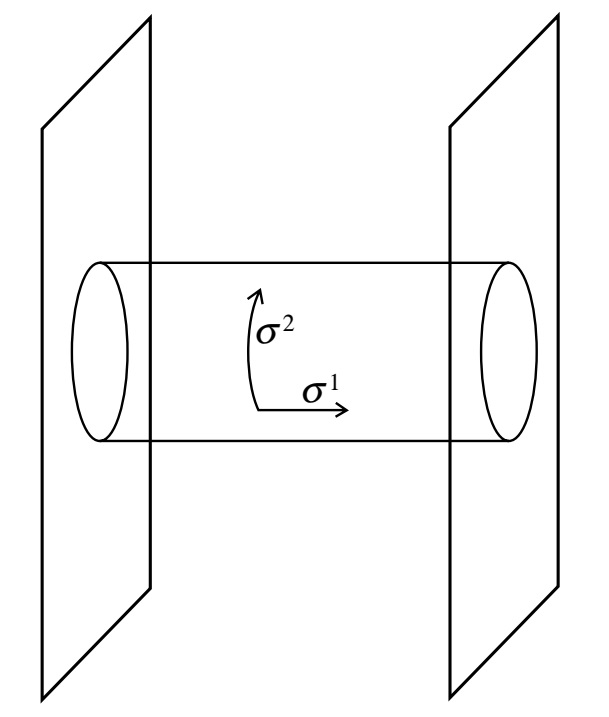
\includegraphics[width=0.6\textwidth]{figure/Fig8.5.jpg}\\
		\caption{Exchanging a closed string between two D-branes. Equivalently, this is the vacuum loop for an open string with endpoints attached to two D-branes.}\label{Fig8.5}
	\end{center}
\end{figure}

In section \ref{sec:7.4}, we calculated the annulus vacuum amplitude using an open string loop, but discovered closed string poles from the $t \rightarrow 0$ limit of the modular integral. 
This is exactly the pole we are interested in, but the simplest way to calculate the amplitude is to treat it as an open string loop. In fact, with a slight change, the previous result \eqref{7.4.1} can be used. 
The number of momentum integrals decreases from 26 to $p{+}1$, and similarly, $V_{26}$ becomes $V_{p+1}$ ; weights $h_{i}$ acquire an extra term $y^{2} / 4\pi^{2} \alpha^{\prime}$ due to stretched open strings; 
the Chan-Paton weight $n^{2}$ becomes 2 (since there are two directions for connecting the strings). 
Therefore we have:
\begin{align}
	\mathscr{A} &= \mi V_{p+1} \int_{0}^{\infty} \frac{\dif t}{t} (8 \pi^{2} \alpha^{\prime} t)^{-(p+1)/2} 
	\exp (-t y^{2} / 2 \pi \alpha^{\prime}) \eta(\mi t)^{-24}  \nonumber \\
	&= \frac{\mi V_{p+1}}{(8 \pi^{2} \alpha^{\prime})^{(p+1)/2}} 
	\int_{0}^{\infty} \dif t\: t^{(21-p)/2} \exp (-t y^{2} / 2 \pi \alpha^{\prime}) \nonumber \\
	& \qquad \qquad \qquad \qquad \qquad  \times[\exp (2 \pi/t)+24+\cdots] \:, \label{8.7.17}
\end{align}
where the asymptotic expansion is obtained by the method in section 7.4. 
The first term is tachyon exchange, thus it is a bosonic artifact. Integrating the second term gives:
\begin{align}
	\mathscr{A} &= \mi V_{p+1} \frac{24}{2^{12}}(4 \pi^{2} \alpha^{\prime})^{11-p} \pi^{(p-23)/2} 
	\Gamma\biggl(\frac{23-p}{2}\biggr)|y|^{p-23}  \nonumber \\
	&= \mi V_{p+1} \frac{24 \pi}{2^{10}}(4 \pi^{2} \alpha^{\prime})^{11-p} G_{25-p}(y) \:, \label{8.7.18}
\end{align}
where $G_{d}(y)$ is the Green function for a massless scalar in $d$ dimensions, the inverse of $-\nabla^{2}$. 
We now want to compare this with the field theory calculation of the same amplitude. Since antisymmetric tensors do not couple to D-branes, from the spacetime action \eqref{3.7.25}, the relevant terms are:
\begin{equation}
	\bm{S}=\frac{1}{2 \kappa^{2}} \int \dif^{26} X \: (-\tilde{G})^{1/2} 
	\biggl(\tilde{\bm{R}}-\frac{1}{6} \nabla_{\mu} \tilde{\Phi} \tilde{\nabla}^{\mu} \tilde{\Phi}\biggr) \:. \label{8.7.19}
\end{equation}
The tildes denote the Einstein metric.
Because this form of action decouples from the dilaton, it is convenient. The dilaton with tildes has been shifted such that its vacuum expectation value is zero. 
In terms of the same variable, the relevant term in the D-brane action \eqref{8.7.2} is:
\begin{equation}
	\bm{S}_{p} = -\tau_{p} \int \dif^{p+1} \xi \: \exp \biggl(\frac{p-11}{12} \tilde{\Phi}\biggr)
	(-\operatorname{det} \tilde{G}_{ab})^{1/2} \:. \label{8.7.20}
\end{equation}
We defined $\tau_{p}=T_{p} \me^{-\Phi_{0}}$; when the background value of the dilaton is $\Phi_{0}$, this is the true physical tension of the D$p$-brane.

The field theory diagram analogous to Figure 8.5 is the exchange of dilatons or gravitons between D-branes. To obtain the propagator, 
we expand the spacetime action up to second order in $h_{\mu\nu}=\tilde{G}_{\mu\nu}-\eta_{\mu\nu}$ and $\tilde{\Phi}$. 
Additionally, for gravity calculation, we need to choose a gauge. 
The simplest gauge for perturbative calculation is:
\begin{equation}
	F_{\nu} \equiv \partial^{\hat{\mu}} h_{\mu \nu}-\frac{1}{2} \partial_{\nu} h^{\hat{\mu}}{}_{\mu}=0 \:, \label{8.7.21}
\end{equation}
where the "hat" indicates using the flat metric $\eta^{\mu \nu}$ to raise and lower indices. 
Expanding the action to second order and adding the gauge fixing term $-F_{\nu} F^{\hat{\nu}} / 4\kappa^{2}$, 
the spacetime action becomes:
\begin{equation}
	\bm{S}=-\frac{1}{8 \kappa^{2}} \int \dif^{26} X \: \biggl( \partial_{\mu} h_{\nu \lambda} 
	\partial^{\hat{\mu}} h^{\hat{\nu} \hat{\lambda}}-\frac{1}{2} \partial_{\mu} h^{\hat{\nu}}{}_{\nu} 
	\partial^{\hat{\mu}} h^{\hat{\lambda}}{}_{\lambda}+\frac{2}{3} \partial_{\mu} \tilde{\Phi} \partial^{\hat{\mu}} \tilde{\Phi}\biggr) \:. \label{8.7.22}
\end{equation}
Observe the kinetic terms, yielding the momentum space propagator:
\begin{subequations} \label{8.7.23}
	\begin{align}
		\langle\tilde{\Phi} \tilde{\Phi}\rangle &=-\frac{(D-2) \mi \kappa^{2}}{4 k^{2}}  \:, \label{8.7.23a} \\
		\langle h_{\mu \nu} h_{\sigma \rho}\rangle &=-\frac{2 \mi \kappa^{2}}{k^{2}}
		\biggl(\eta_{\mu \sigma} \eta_{\nu \rho}+\eta_{\mu \rho} \eta_{\nu \sigma}-\frac{2}{D-2} \eta_{\mu \nu} \eta_{\sigma \rho}\biggr) \:. \label{8.7.23b}
	\end{align}
\end{subequations}
For later reference, we gave general $D$. Expanding around a general flat configuration, the D-brane action is:
\begin{equation}
	\bm{S}_{p}=-\tau_{p} \int \dif^{p+1} \xi \: \biggl(\frac{p-11}{12} \tilde{\Phi}-\frac{1}{2} h_{aa}\biggr) \:. \label{8.7.24}
\end{equation}
Note that $h_{\mu \nu}$ here is traced only over directions tangent to the D-brane; we have taken $\xi$ as Cartesian coordinates with metric $\delta_{ab}$. 
We can now read the Feynman diagram:
\begin{align}
	\mathscr{A} &= \frac{\mi \kappa^{2} \tau_{p}^{2}}{k_{\perp}^{2}} V_{p+1} 
	\left\{6\left[\frac{p-11}{12}\right]^{2}+\frac{1}{2}\left[2(p+1)-\frac{1}{12}(p+1)^{2}\right]\right\} \nonumber \\
	& =\frac{6 \mi \kappa^{2} \tau_{p}^{2}}{k_{\perp}^{2}} V_{p+1} \:. \label{8.7.25}
\end{align}
\begin{tcolorbox}
	\begin{remark}
		The above comes from $\langle S_p S_p \rangle$.
	\end{remark}	
\end{tcolorbox}
\noindent Comparison with \eqref{8.7.18} gives:
\begin{equation}
	\tau_{p}^{2} = \frac{\pi}{256 \kappa^{2}} (4 \pi^{2} \alpha^{\prime})^{11-p} \:. \label{8.7.26}
\end{equation}
This is consistent with the recurrence relation given by $T$-duality.

As an application, consider a state with $n$ 25-branes, which is identical to the ordinary $n$-valued Chan-Paton factor. 
Expanding the 25-brane action \eqref{8.7.12} to second order in the gauge field yields:
\begin{equation}
	\frac{\tau_{25}}{4}(2 \pi \alpha^{\prime})^{2} \operatorname{Tr}(F_{\mu \nu} F^{\mu \nu}) \:. \label{8.7.27}
\end{equation}
This relates the open string gauge coupling and closed string gravitational coupling. 
Using \eqref{6.5.14}, \eqref{6.5.16}, \eqref{6.6.15}, and \eqref{6.6.18}, 
we can write this as a relationship between the vertex operator normalizations $g_{\mathrm{c}}$ and $g_{\mathrm{o}}$:
\begin{equation}
	\frac{g_{\mathrm{o}}^{2}}{g_{\mathrm{c}}} = \frac{4 \pi \alpha^{\prime} g_{\mathrm{o}}^{\prime 2}}{\kappa}
	= 2^{18} \pi^{25 / 2} \alpha^{\prime 6} \:. \label{8.7.28}
\end{equation}
It has the correct form, with the square of the open string coupling being proportional to the closed string coupling, but now with a numerical coefficient. We decompose closed string poles from the torus via unitarity, or see Exercise 7.9.

\section{\texorpdfstring{$T$-duality of Unoriented Theories}{8.8 $T$-duality of Unoriented Theories}} \label{sec:8.8}
In unoriented string theory, the $R \rightarrow 0$ limit also yields interesting new physics. First consider the closed string theory. To form an unoriented theory, we impose $\Omega=+1$ on the states. 
Following the discussion in section 8.5, we can also think of this as gauging $\Omega$. In particular, the transition functions used to construct the worldsheet now reverse directions, and this produces an unoriented worldsheet.

The $T$-dual theory is obtained by replacing $X^{m}(z, \bar{z})=X_{L}^{m}(z)+X_{R}^{m}(\bar{z})$ with coordinates $X^{\prime m}(z, \bar{z})= X_{L}^{m}(z)-X_{R}^{m}(\bar{z})$. 
In the original description, we gauge worldsheet parity $\Omega$, whose action is:
\begin{equation}
	\Omega: X_{L}^{M}(z) \leftrightarrow X_{R}^{M}(z) \:. \label{8.8.1}
\end{equation}
In $T$-dual coordinates, this is:
\begin{subequations} \label{8.8.2}
	\begin{align}
		\Omega: \quad X^{\prime m}(z, \bar{z})  &\leftrightarrow-X^{\prime m}(\bar{z}, z) \:, \label{8.8.2a} \\
		X^{\mu}(z, \bar{z})  &\leftrightarrow X^{\mu}(\bar{z}, z) \:, \label{8.8.2b}
	\end{align}
\end{subequations}
as before, $m$ labels coordinates for which $T$-duality is taken, and $\mu$ labels coordinates for which $T$-duality is not taken. 
In the dual picture, symmetry \eqref{8.8.2} is thus the product of worldsheet parity transformation and spacetime inversion. 
We see that gauging worldsheet parity only produces an unoriented theory, while gauging inversion only produces an orbifold. The result of the combined projection is called an \emph{orientifold}.

An orientifold is very similar to an orbifold. Divide the string wave function into its interior and its center-of-mass $x^{m}$ dependent part, taking the interior wave function to be an eigenstate of $\Omega$. 
Then the projection onto $\Omega=+1$ indicates that the string wave function at $-x^{m}$ is the same as at $x^{m}$, differing only by a sign. 
For example, the components of the metric and antisymmetric tensor satisfy:
\begin{subequations} \label{8.8.3}
	\begin{align}
		G_{\mu \nu}(x^{\prime}) &= G_{\mu \nu}(x) \:, \quad  B_{\mu \nu}(x^{\prime})=-B_{\mu \nu}(x) \:, \label{8.8.3a} \\ 	
		G_{\mu n}(x^{\prime}) & =-G_{\mu n}(x) \:, \quad  B_{\mu n}(x^{\prime})=B_{\mu n}(x) 	\:, \label{8.8.3b} \\
		G_{m n}(x^{\prime}) &= G_{m n}(x) \:, \quad  B_{m n}(x^{\prime})=-B_{m n}(x) \:, \label{8.8.3c}
	\end{align}
\end{subequations}
where $(x^{\mu}, x^{m})^{\prime} = (x^{\mu},-x^{m})$. 
There is one negative sign for each of $m, n$ and another negative sign for $B_{M N}$; this is identical to an orbifold. 
In other words, the $T$-dual spacetime is the torus $T^{k}$ modulo the $\mathds{Z}_{2}$ reflection in $k$ compact dimensions, exactly the same as the construction of an orbifold. 
For example, if there is only one periodicity, the dual spacetime is the segment $0 \leq x^{25} \leq \pi R^{\prime}$, with orientifold fixed planes at the ends.

Note that when away from the orientifold fixed plane, the local physics is that of an oriented string theory. Unlike the original unoriented theory, where projection locally removes half of the states, 
here it relates the string wave function at any point to its value at the mirror point, as in \eqref{8.8.3}. 
One difference between orientifold and orbifold constructions is that the former has no direct analogue of twisted states because the Klein bottle has no modular transformation $\tau \rightarrow -1/\tau$. Examine Figure 8.6, which shows the torus and the Klein bottle. On the torus, the projection operator inserts a twist in the time-like direction in Figure 8.6a; rotating this figure by $90^{\circ}$, 
this becomes a twist in the spatial direction, implying the existence of twisted states in the spectrum. However, if the Klein bottle in Figure 8.6b is rotated by $90^{\circ}$, the time directions on relative sides cannot match. 
So there is no intermediate state interpretation in this channel. Thus it should be noted that the orientifold plane cannot be dynamical. Unlike the D-brane case, no string modes are tethered to the orientifold plane to represent its shape fluctuations. 
Our heuristic discussion—that gravitational waves force D-branes to oscillate here—does not apply to orientifold planes. Ultimately, the equivalence relation \eqref{8.8.3} becomes a boundary condition on fixed planes, causing incident waves to cancel with reflected waves. 
For D-branes, the reflected wave is a higher-order quantity of the string coupling.

\begin{figure}[!htbp]
	\begin{center}
		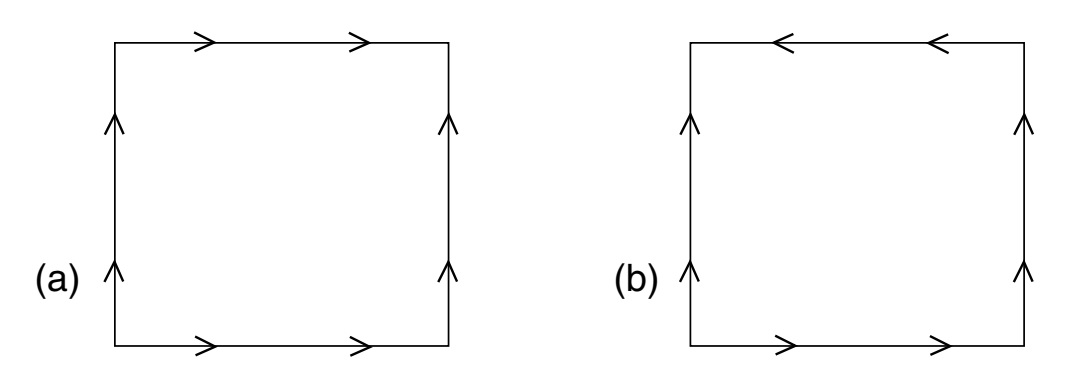
\includegraphics[width=0.8\textwidth]{figure/Fig8.6.jpg}
		\caption{Gluing opposite sides gives (a) a torus and (b) a Klein bottle.}\label{Fig8.6}
	\end{center}
\end{figure}

In drawing oriented strings, we use arrows to indicate directions. In unoriented theory, we can either omit the arrows or take a linear combination of the two directions. 
The latter picture is more consistent with the idea of gauging discrete symmetries and is more widespread: in an orientifold, parity operators must be accompanied by a spacetime transformation, so we cannot simply forget the arrows.

Although we introduced orientifold construction through $T$-duality, one can also examine orientifolds that are not $T$-duals of toroidal compactifications, combining worldsheet parity with various spacetime symmetries to gauge a group.

\subsection*{Open Strings}

In the case of open strings, the situation is similar. For simplicity, we only examine the case of one compact dimension. As before, there are orientifold fixed planes at 0 and $\pi R^{\prime}$. 
Introduce $SO(n)$ Chan-Paton factors (symplectic symmetry is similar), and a general Wilson line can be transformed into a diagonal form; when $n$ is even, the eigenvalues appear in pairs: 
\begin{equation}
	W = \operatorname{diag}\left(\me^{\mi \theta_{1}}, \me^{-\mi \theta_{1}}, \me^{\mi \theta_{2}}, \me^{-\mi \theta_{2}}, \cdots, 
	\me^{\mi \theta_{n/2}}, \me^{-\mi \theta_{n/2}}\right) \:. \label{8.8.4}
\end{equation}
Thus, in the dual picture, there are $\frac{1}{2} n$ D-branes in the segment $0 \leq X^{\prime 25} \leq \pi R^{\prime}$, and another $\frac{1}{2} n$ at mirror points. 
Strings can open between D-branes and mirrors, as shown in Figure \ref{Fig8.7}.
The general gauge group is $U(1)^{n/2}$. Similar to oriented theory, if $r$ D-branes coincide, then a $U(r)$ gauge group exists. 
If these $r$ D-branes are also on one of the fixed planes, then strings opening between one of these branes and its mirror brane are also massless. We would then have the correct spectrum of extra states to fill $SO(2r)$. 
If all branes are on an orientifold plane, the maximum $SO(n)$ is restored. 

\begin{figure}[!htbp]
	\begin{center}
		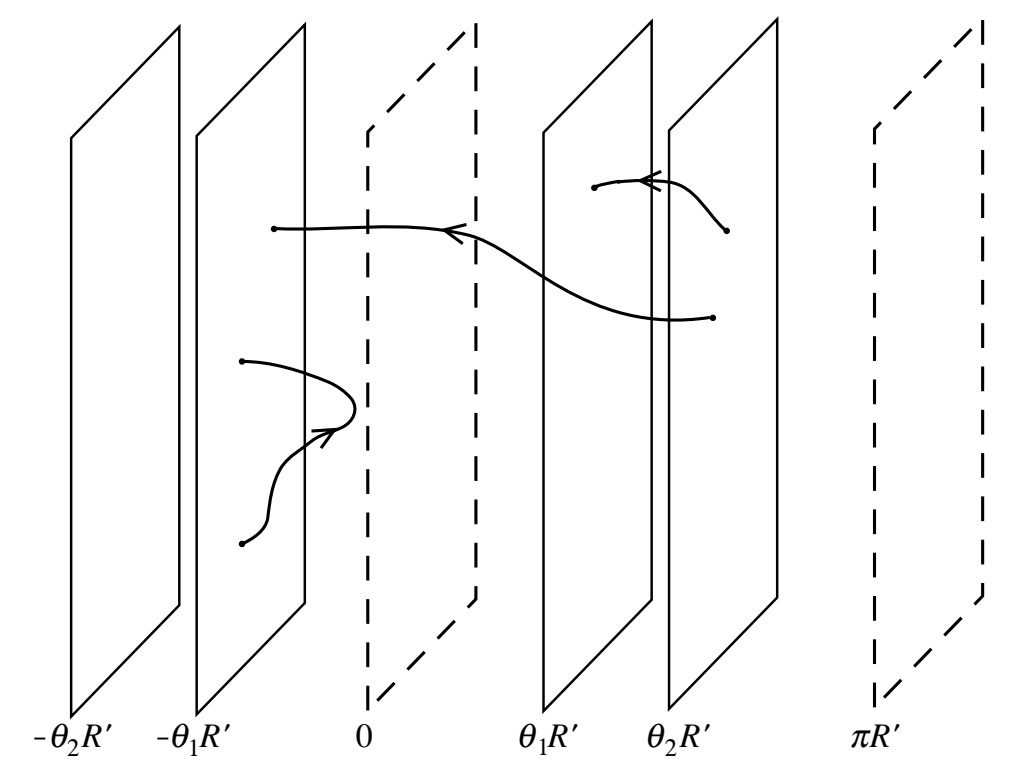
\includegraphics[width=0.6\textwidth]{figure/Fig8.7.jpg}
		\caption{Orientifold planes are at 0 and $\pi R^{\prime}$, D-branes are at $\theta_{1} R^{\prime}$ and $\theta_{2} R^{\prime}$, 
			and D-brane images are at $-\theta_{1} R^{\prime}$ and $-\theta_{2} R^{\prime}$. The effect of the twisting operator $\Omega$ on any string is a combination of spacetime reversal and reversal of oriented arrows.
		}\label{Fig8.7}
	\end{center}
\end{figure}

If $n$ is odd, the last eigenvalue of $W$ is $\pm 1$, causing it to be fixed on one of the two orientifold planes in the $T$-dual picture. 
Without mirrors, this is actually a half-D-brane. 
Additionally, if we examine the $n=2$ Wilson line $\operatorname{diag}(1,-1)$ (which is in $O(2)$ instead of $SO(2)$), what appears is not one D-brane and its image, but two half-D-branes.

As with D-branes, orientifold planes couple with the dilaton and metric. 
The amplitude is the same as in the previous section, except for replacing the annulus with Klein bottles and Möbius strips. 
In fact, we already performed relevant calculations in Chapter 7. There we found the total dilaton coupling cancels for $S O\left(2^{13}\right)$. 
In the $T$-dual picture, the total dilaton coupling of $2^{12}$ D-branes cancels (images are not included in the count). If we compactify $k=25-p$ dimensions, there will be $2^{k}$ fixed planes, 
whose coordinates are all combinations of 0 and $\pi R_{m}^{\prime}$. 
Thus the effective action of a single fixed plane is:
\begin{equation}
	2^{12-k} T_{p} \int \dif^{p+1} \xi \: \me^{-\Phi} (-\operatorname{det} G_{ab})^{1/2} \:, \label{8.8.5}
\end{equation}
where integration runs over fixed planes.

Although there is no direct analogue of twisted sectors in orientifolds, in some sense, twisted states are open strings. Since this analogy is not complete, we do not tend to emphasize it: 
gauging $\Omega$ itself does not introduce worldsheet boundaries. 
However, adding open strings to an orientifold theory to cancel the dilaton tadpole has certain physical significance. This cancellation will play an important role in superstrings.